\chapter{中国重症加强治疗病房(ICU)建设与管理指南(2006)}

\textbf{中华医学会重症医学分会}

一、引言

二、基本要求

三、ICU的规模

四、ICU的人员配备

五、ICU医护人员专业要求

六、ICU的医疗管理

七、ICU病房建设标准

八、ICU必配设备

九、ICU选配设备

\section{引 言}

重症医学(critical care
medicine,CCM)是研究危及生命的疾病状态的发生、发展规律及其诊治方法的临床医学学科。重症加强治疗病房(intensive
care
unit,ICU)是重症医学学科的临床基地,它对因各种原因导致一个或多个器官与系统功能障碍危及生命或具有潜在高危因素的患者,及时提供系统的、高质量的医学监护和救治技术,是医院集中监护和救治重症患者的专业科室。ICU应用先进的诊断、监护和治疗设备与技术,对病情进行连续、动态的定性和定量观察,并通过有效的干预措施,为重症患者提供规范的、高质量的生命支持,改善生存质量。重症患者的生命支持技术水平,直接反映医院的综合救治能力,体现医院整体医疗实力,是现代化医院的重要标志。重症医学的学科建设和ICU的组织与管理,应该符合国家有关标准。

为促进我国重症医学的发展,规范我国医疗机构ICU的组织与管理,特制订《中国重症加强治疗病房(ICU)建设与管理指南》。

\section{基本要求}

(1)我国三级和有条件的二级医院均应设立重症医学科,重症医学科属于临床独立学科,直属医院职能部门直接领导。ICU是重症医学学科的临床基地。

(2)ICU必须配备足够数量、受过专门训练、掌握重症医学基础知识和基本操作技术、具备独立工作能力的专职医护人员。

(3)ICU必须配置必要的监护和治疗设备,接收医院各科的重症患者。

\section{ICU的规模}

ICU的病床数量根据医院等级和实际收治患者的需要,一般以该ICU服务病床数或医院病床总数的2%~8%为宜,可根据实际需要适当增加。从医疗运作角度考虑,每个ICU管理单元以8到12张床位为宜;床位使用率以65%~75%为宜,超过80%则表明ICU的床位数不能满足医院的临床需要,应该扩大规模。

\section{ICU的人员配备}

(1)ICU专科医师的固定编制人数与床位数之比为0.8~1∶1以上。ICU日常工作中可有部分轮科、进修医师。ICU医师组成应包括高级、中级和初级医师,每个管理单元必须至少配备一名具有高级职称的医师全面负责医疗工作。

(2)ICU专科护士的固定编制人数与床位数之比为2.5~3∶1以上。

(3)ICU可以根据需要配备适当数量的医疗辅助人员,有条件的医院可配备相关的技术与维修人员。

\section{ICU医护人员专业要求}

(1)ICU医师应经过严格的专业理论和技术培训,以胜任对重症患者进行各项监测与治疗的要求。

(2)ICU医师应经过规范化的相关学科轮转培训。

(3)ICU医师必须具备重症医学相关理论知识。掌握重要脏器和系统的相关生理、病理及病理生理学知识、ICU相关的临床药理学知识和伦理学概念。

(4)ICU医师应掌握重症患者重要器官、系统功能监测和支持的理论与技能:①复苏;②休克;③呼吸功能衰竭;④心功能不全、严重心律失常;⑤急性肾功能不全;⑥中枢神经系统功能障碍;⑦严重肝功能障碍;⑧胃肠功能障碍与消化道大出血;⑨急性凝血功能障碍;⑩严重内分泌与代谢紊乱;⑪水电解质与酸碱平衡紊乱;⑫肠内与肠外营养支持;⑬镇静与镇痛;⑭严重感染;⑮多器官功能障碍综合征;⑯免疫功能紊乱。

(5)ICU医师除一般临床监护和治疗技术外,应具备独立完成以下监测与支持技术的能力:①心肺复苏术;②人工气道建立与管理;③机械通气技术;④纤维支气管镜技术;⑤深静脉及动脉置管技术;⑥血流动力学监测技术;⑦胸穿、心包穿刺术及胸腔闭式引流术;⑧电复律与心脏除颤术;⑨床旁临时心脏起搏技术;⑩持续血液净化技术;⑪疾病危重程度评估方法。

(6)ICU医师每年至少参加一次省级或省级以上重症医学相关继续医学教育培训项目的学习,不断加强知识更新。

(7)ICU护士必须经过严格的专业培训,熟练掌握重症护理基本理论和技能,经过专科考核合格后,才能独立上岗。

\section{ICU的医疗管理}

(1)ICU必须建立健全各项规章制度,制定各类人员的工作职责,规范诊疗常规。除执行政府和医院临床医疗的各种制度外,应该制订以下符合ICU相关工作特征的制度,以保证ICU的工作质量:①医疗质量控制制度;②临床诊疗及医疗护理操作常规;③患者转入、转出ICU制度;④抗生素使用制度;⑤血液与血液制品使用制度;⑥抢救设备操作、管理制度;⑦特殊药品管理制度;⑧院内感染控制制度;⑨不良医疗事件防范与报告制度;⑩疑难重症患者会诊制度;⑪医患沟通制度;⑫突发事件的应急预案、人员紧急召集制度。

(2)ICU的患者由ICU医生负责管理。患者的相关专科情况,ICU医生应该与专科医生共同协商处理。

(3)ICU的收治范围:①急性、可逆、已经危及生命的器官功能不全,经过ICU的严密监护和加强治疗短期内可能得到康复的患者;②存在各种高危因素,具有潜在生命危险,经过ICU严密的监护和随时有效治疗可能减少死亡风险的患者;③在慢性器官功能不全的基础上,出现急性加重且危及生命,经过ICU的严密监护和治疗可能恢复到原来状态的患者;④慢性消耗性疾病的终末状态、不可逆性疾病和不能从ICU的监护治疗中获得益处的患者,一般不是ICU的收治范围。

\section{ICU病房建设标准}

(1)ICU应该有特殊的地理位置,设置于方便患者转运、检查和治疗的区域并考虑以下因素:接近主要服务对象病区、手术室、影像学科、化验室和血库等,在横向无法实现“接近”时,应该考虑楼上楼下的纵向“接近”。

(2)ICU开放式病床每床的占地面积为15~18m\textsuperscript{2}
;每个ICU最少配备一个单间病房,面积为18~25m\textsuperscript{2}
。每个ICU中的正压和负压隔离病房的设立,可以根据患者专科来源和卫生行政部门的要求决定,通常配备负压隔离病房1~2间。鼓励在人力资源充足的条件下,多设计单间或分隔式病房。

(3)ICU的基本辅助用房包括医师办公室、主任办公室、工作人员休息室、中央工作站、治疗室、配药室、仪器室、更衣室、清洁室、污废物处理室、值班室、盥洗室等。有条件的ICU可配置其他辅助用房,包括示教室、家属接待室、实验室、营养准备室等。辅助用房面积与病房面积之比应达到1.5∶1以上。

(4)ICU的整体布局应该使放置病床的医疗区域、医疗辅助用房区域、污物处理区域和医务人员生活辅助用房区域等有相对的独立性,以减少彼此之间的互相干扰并有利于感染的控制。

(5)ICU应具备良好的通风、采光条件,有条件者最好装配气流方向从上到下的空气净化系统,能独立控制室内的温度和湿度。医疗区域内的温度应维持在24±1.5℃。每个单间的空气调节系统应该独立控制。安装足够的感应式洗手设施和手部消毒装置,单间每床1套,开放式病床至少每2床1套。

(6)ICU要有合理的包括人员流动和物流在内的医疗流向,最好通过不同的进出通道实现,以最大限度减少各种干扰和交叉感染。

(7)ICU病房建筑装饰必须遵循不产尘、不积尘、耐腐蚀、防潮防霉、防静电、容易清洁和符合防火要求的总原则。

(8)ICU的设计要求应该满足提供医护人员便利的观察条件和在必要时尽快接触病人的通道。

(9)除了患者的呼叫信号、监护仪器的报警声外,电话铃声、打印机等仪器发出的声音等均属于ICU的噪音。在不影响正常工作的情况下,这些声音应尽可能减少到最小的水平。根据国际噪音协会的建议,ICU白天的噪音最好不要超过45dB(A),傍晚40dB(A),夜晚20dB(A)。地面覆盖物、墙壁和天花板应该尽量采用高吸音的建筑材料。

(10)ICU应建立完善的通讯系统、网络与临床信息管理系统、广播系统。

\section{ICU必配设备}

(1)每床配备完善的功能设备带或功能架,提供电、氧气、压缩空气和负压吸引等功能支持。每张监护病床装配电源插座12个以上,氧气接口2个以上,压缩空气接口2个和负压吸引接口2个以上。医疗用电和生活照明用电线路分开。每个ICU床位的电源应该是独立的反馈电路供应。ICU最好有备用的不间断电力系统(UPS)和漏电保护装置;最好每个电路插座都在主面板上有独立的电路短路器。

(2)应配备适合ICU使用的病床,配备防褥疮床垫。

(3)每床配备床旁监护系统,进行心电、血压、脉搏血氧饱和度、有创压力监测等基本生命体征监护。为便于安全转运患者,每个ICU单元至少配备便携式监护仪1台。

三级医院的ICU应该每床配备1台呼吸机,二级医院的ICU可根据实际需要配备适当数量的呼吸机。每床配备简易呼吸器(复苏呼吸气囊)。为便于安全转运患者,每个ICU单元至少应有便携式呼吸机1台。

(4)输液泵和微量注射泵每床均应配备,其中微量注射泵每床2套以上。另配备一定数量的肠内营养输注泵。

(5)其他设备:心电图机、血气分析仪、除颤仪、血液净化仪、连续性血流动力学与氧代谢监测设备、心肺复苏抢救装备车(车上备有喉镜、气管导管、各种接头、急救药品以及其他抢救用具等)、体外起搏器、纤维支气管镜、电子升降温设备等。

(6)医院或ICU必须有足够的设备,随时为ICU提供床旁B超、X光、生化和细菌学等检查。

\section{ICU选配设备}

除上述必配设备外,有条件者,视需要可选配以下设备:

(1)易生化仪和乳酸分析仪。

(2)闭路电视探视系统,每床一个成像探头。

(3)脑电双频指数监护仪(BIS)。

(4)输液加温设备。

(5)胃黏膜二氧化碳张力与pHi测定仪。

(6)呼气末二氧化碳、代谢等监测设备。

(7)体外膜肺(ECMO)。

(8)床边脑电图和颅内压监测设备。

(9)主动脉内球囊反搏(IABP)和左心辅助循环装置。

(10)防止下肢DVT发生的反搏处理仪器。

(11)胸部震荡排痰装置。

《中国重症加强治疗病房(ICU)建设与管理指南》经过中华医学会重症医学分会反复酝酿、讨论制订,随着我国重症医学的发展与进步,本会将根据我国的实际情况适时做出修订。

\textbf{中华医学会重症医学分会}

《中国重症加强治疗病房(ICU)建设与管理指南(2006)》工作组

组长:管向东

组员(按姓氏笔画为序):于凯江(哈尔滨医科大学附属第一医院),马晓春(中国医科大学附属第一医院),方强(浙江大学附属第一医院),刘大为(中国医学科学院北京协和医院),安友仲(北京大学人民医院),邱海波(东南大学附属中大医院),严静(浙江医院),康焰(四川大学附属华西医院),覃铁和(广东省人民医院),管向东(中山大学附属第一医院)

\protect\hypertarget{text00033.html}{}{}

\chapter{成人严重感染与感染性休克血流动力学监测与支持指南(2006)}

\textbf{中华医学会重症医学分会}

一、引言

二、严重感染与感染性休克的血流动力学改变特点

三、严重感染与感染性休克的诊断

四、严重感染与感染性休克的血流动力学监测目的与意义

五、常用监测指标的选择与影响因素

六、功能性血流动力学监测

七、严重感染与感染性休克的血流动力学支持

八、严重感染与感染性休克的集束化治疗

\section{引 言}

严重感染(severe sepsis)及其相关的感染性休克(septic
shock)和多脏器功能障碍综合征(multiple organ dysfunction
syndrome,MODS)是当前重症加强治疗病房(ICU)内主要的死亡原因,也是当代重症医学面临的主要焦点及难点。在美国,每年有75万的严重感染病例发生,超过了充血性心力衰竭或乳腺癌、结肠癌和艾滋病的患病数总和,病死率大概在20%~63%,和急性心肌梗死的院外病死率相近,且患病率以每年1.5%的比例增长,预计到2010和2020年,严重感染的患病数将达到93万和110万。美国每年的相关治疗费用大约为167亿美元,而欧洲每年的相关治疗费用大约为94亿美元。在全球范围内,严重感染病例的患病率、病死率及相关治疗费用也在逐年增加,全球每年有1800万人发生严重感染,每天大约有1400人死于严重感染。尽管国内尚无完整的流行病学资料,但据估计患病率、病死率、治疗费用也相当高。人口老龄化和慢性病的增加,人类的医疗活动如肿瘤化疗和器官移植后免疫抑制剂的应用都是导致严重感染发病率增加的重要原因。

严重感染与感染性休克以高心输出量和低外周血管阻力并导致组织灌注不足为特征,其血流动力学的复杂性使支持目标的实现更为困难。因此,血流动力学的监测与分析并根据血流动力学指标的变化给予及时支持就显得尤为重要。显然,治疗效果应该通过监测综合参数来评估,而临床医生应该有明确的目标和治疗终点以评价当前干预的效果。

为使重症医学工作者对成人严重感染与感染性休克的血流动力学监测与支持的时机、方法与目标有一个全面、系统的认识,以便进行规范化的临床实施,中华医学会重症医学分会组织相关专家,依据近年来国内外研究进展和临床实践,制定以下《成人严重感染与感染性休克血流动力学监测与支持指南》。

本《指南》的推荐意见采用循证医学的方法,推荐级别依据如表\ref{tabapp-1}。

\begin{longtable}{c}
  \caption{推荐级别与研究文献的Delphi分级}
  \label{tabapp-1}
  \endfirsthead
  \caption[]{推荐级别与研究文献的Delphi分级}
  \endhead
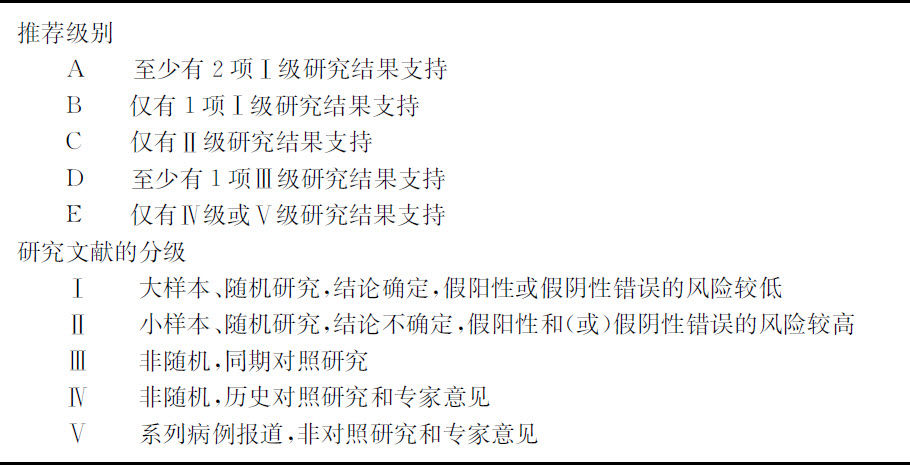
\includegraphics[width=\textwidth,height=\textheight,keepaspectratio]{./images/Image00299.jpg}
\end{longtable}

\section{严重感染与感染性休克的血流动力学特点}

严重感染和感染性休克时,循环系统主要表现为体循环阻力下降,同时伴有心输出量正常或增加,肺循环阻力通常略有升高。体循环阻力下降被认为是感染性休克的首要血流动力学改变,这种状态通常被称之为高动力型血流动力学状态。严重感染常导致左右心室的功能受到明显抑制,可表现为心室射血分数下降,心肌顺应性下降。

严重感染和感染性休克的血流动力学改变的基础,是外周血管的收缩舒张功能的异常,从而导致血流的分布异常。在感染性休克发生的早期,由于血管的扩张和通透性的改变,可出现循环系统的低容量状态。经过容量补充后,血流动力学则表现为高动力状态。外周阻力下降、心输出量正常或升高,作为循环高流量和高氧输送的形成基础而成为感染性休克的主要特点。感染性休克的这种氧输送正常或增高状态下的组织缺氧是分布性休克的主要特征,与低容量性休克、心源性休克和梗阻性休克氧输送减少的特点有明确的不同。

严重感染时,组织对氧的摄取和利用功能也发生改变。微循环的功能改变及组织代谢功能障碍可以存在于感染过程的始终。炎症反应导致毛细血管内皮系统受损、凝血功能异常、血管通透性增加,使血管内容量减少、组织水肿;组织内通血微血管密度下降,无血流和间断血流的微血管比例增加。这些改变直接导致微循环和组织间的物质交换障碍,在器官功能不全的发展过程中起着关键作用。同时,炎症反应导致的线粒体功能障碍使细胞对氧的利用也受到明显的影响。这些改变的共同作用使组织缺氧及代谢功能障碍进行性加重,加速了休克的发展。

推荐意见1:感染性休克以血流分布异常为主要血流动力学特点,应注意在整体氧输送不减少情况下的组织缺氧。(E级)

\section{严重感染与感染性休克的诊断}

严重感染和感染性休克通常表现为一个进行性发展的临床过程。这个过程的不同阶段可以表现出不同的特点。为了能够更早期对严重感染和感染性休克进行识别和诊断,人们做了大量的工作,并不断形成新的共识。

1991年8月美国胸科医师学会(ACCP)和重症医学会(SCCM)联席会议对全身炎症反应综合征(SIRS)规定了明确的定义和诊断标准:SIRS是机体对不同的严重损伤所产生的全身性炎性反应。这些损伤可以是感染,也可以是非感染性损伤,如严重创伤、烧伤,胰腺炎等等。如出现两种或两种以上的下列表现,可以认为有这种反应的存在:①体温>38℃或<36℃;②心率>90次/分;③呼吸频率>20次/分,或动脉血二氧化碳分压<32mmHg(4.3kPa);④血白细胞>12×10\textsuperscript{9}
/L、<4×10\textsuperscript{9}
/L或幼稚型细胞>10%。会议同时指出,由致病微生物所引起的SIRS为全身性感染(sepsis);严重感染是指全身性感染伴有器官功能不全、组织灌注不良或低血压。感染性休克可以被认为是严重感染的一种特殊类型。

临床上沿用的诊断感染性休克的标准常包括:①临床上有明确的感染;②有SIRS的存在;③收缩压低于90mmHg或较原基础值下降的幅度超过40mmHg,至少1小时,或血压依赖输液或药物维持;④有组织灌注不良的表现,如少尿(<30ml/小时)超过1小时,或有急性神志障碍。这些指标在今天看来,尚不能完全体现对感染性休克作为临床过程的认识和早期诊断的要求。

2001年有关方面的专家对相关的概念进行重新论证,认为虽然这些定义在临床应用方面存有一定缺陷。但尚无足够的证据改变1991年所制定的这些定义。临床上需要更具体的指标(如生物学指标)对全身性感染的严重程度进行更为明确的区分。会议建议应用PIRO系统,希望提供更清晰的、定量化的诊断标准。PIRO系统包括易感性(predisposition)、感染侵袭(insult
infection)、机体反应(response)和器官功能不全(organ
dysfunction)。该系统相应的反映:①病人的基础情况、对炎症反应的基因特征;②致病微生物的药物敏感性和分子生物学特征,感染源的部位、严重程度和对治疗的反应;③机体炎症反应特点和特异性生物学指标(如降钙素前体、C反应蛋白、人类白细胞相关性抗原、白介素等)的意义;④器官受累的数量、程度及其相应的评分系统。

从对感染过程的认识和对感染性休克的定位,可以看出一些基本概念的转变。这种转变正在影响着对感染性休克的诊断和临床治疗的决策。

推荐意见2:应重视严重感染和感染性休克是一个进行性发展的临床过程,对这个过程的认识有助于早期诊断。(E级)

\section{严重感染与感染性休克血流动力学监测的目的与意义}

血流动力学的监测对严重感染与感染性休克的早期诊断、预后的判断以及治疗过程中效果的观察、方案的反馈与调整至关重要,早期合理地选择监测指标并正确解读有助于指导严重感染与感染性休克患者的治疗。常规血流动力学监测可以用于基础循环状态、容量复苏和药物治疗效果的评价,其核心内容是组织灌注与氧代谢状况,包括全身和局部灌注指标的监测。

常规血流动力学监测包括体循环的监测参数:心率、血压、中心静脉压(CVP)与心排血量和体循环阻力(SVR)等;肺循环监测参数:肺动脉压(PAP)、肺动脉嵌压(PAWP)和肺循环阻力(PVR)等;氧动力学与代谢监测参数:氧输送(DO\textsubscript{2}
)、氧消耗(VO\textsubscript{2}
)等;氧代谢监测参数:血乳酸、脉搏氧饱和度、混合静脉血氧饱和度(SvO\textsubscript{2}
)或中心静脉血氧饱和度(ScvO\textsubscript{2}
)的监测等。严重感染与感染性休克时组织持续缺氧,传统临床监测指标如心率、血压、尿量、神志、毛细血管充盈状态、皮肤灌注等往往不能对组织氧合的改变具有敏感的反应。此外,经过治疗干预后的心率、血压等临床指标的变化也可在组织灌注与氧合未改善前趋于稳定。因此,监测和评估全身灌注指标(DO\textsubscript{2}
、VO\textsubscript{2} 、Lac、ScvO\textsubscript{2}
或ScvO\textsubscript{2}
等)以及局部组织灌注指标(胃黏膜pH值测定或消化道黏膜PCO\textsubscript{2}
测定等)很有必要。

临床上,中心静脉压、肺动脉嵌顿压和心室舒张末容积是常用的反映心脏前负荷的参数,体循环阻力(SVR)为监测左心室后负荷的指标,肺循环阻力(PVR)为监测右心室后负荷的指标,每搏输出量、心室每搏做功指数、射血分数等指标反映了心肌收缩力的变化情况。

监测CVP对右心容量的调整起到了一定的指导作用,但在反映左心前负荷方面仍有较大的局限性。相比之下,PAWP与左心前负荷的变化更具有相关性。但是,CVP与PAWP都是通过以压力代容积的方法来反映心脏前负荷的,会受到心室顺应性的影响。从理论上讲,直接监测心室舒张末容积是最理想的反映心脏前负荷的指标。肺动脉漂浮导管(Swan-Ganz导管)是血流动力学监测的有效手段,通过漂浮导管获取的参数资料,可以更好地指导临床治疗。近年来有些研究显示肺动脉漂浮导管会增加病人的并发症,使死亡率升高,但也有随机、多中心、大规模、前瞻性临床研究表明,肺动脉漂浮导管在危重病治疗中对病人的死亡率、总住院时间、ICU住院时间、器官支持治疗时间均无影响,研究者分析认为:医务人员对漂浮导管数据的误解、无效的治疗方案、缺乏更全面的知识培训是肺动脉漂浮导管不能给危重病人带来益处的主要原因。

综合评价DO\textsubscript{2} 、VO\textsubscript{2}
及两者的相关性可以实现组织氧动力学的优化治疗,氧摄取率(O\textsubscript{2}
ER)作为评价氧供需平衡的指标,其效果比单纯应用DO\textsubscript{2}
和VO\textsubscript{2} 更敏感。正常情况下,DO\textsubscript{2}
改变时,因为氧摄取率的变化,VO\textsubscript{2}
保持不变,也就是说VO\textsubscript{2} 不受DO\textsubscript{2}
的影响。但当DO\textsubscript{2} 下降到一临界值时,VO\textsubscript{2}
依赖于DO\textsubscript{2} 的变化,O\textsubscript{2}
ER的增加也无法满足组织氧合,于是就发生无氧代谢。另外,O\textsubscript{2}
ER可以作为判断患者预后的指标。混合静脉血氧饱和度(SvO\textsubscript{2}
)反映DO\textsubscript{2} 和VO\textsubscript{2}
的平衡,当DO\textsubscript{2} 不能满足组织氧需要时SvO\textsubscript{2}
下降。严重感染与感染性休克时,可因为血流分布不均或组织氧利用障碍使SvO\textsubscript{2}
升高,所以SvO\textsubscript{2}
值需要与其他血流动力学指标一起解读。近期研究认为,监测中心静脉血氧饱和度(ScvO\textsubscript{2}
)对于指导早期复苏有重要价值。血乳酸作为全身灌注与氧代谢的重要指标,它的升高反映了低灌注情况下无氧代谢的增加。血乳酸水平升高在预测严重感染与感染性休克病人的预后方面很有价值,血乳酸清除率比单一的血乳酸值更有意义。

临床上局部灌注的评估经常靠评价器官功能来实现,如心肌缺血,尿量减少,血尿素氮和肌酐的升高,神志异常,血清转氨酶、乳酸脱氢酶、胆红素的升高和凝血酶原时间的延长等。严重感染与感染性休克病人组织灌注减少,CO\textsubscript{2}
积蓄与清除障碍,消化道CO\textsubscript{2}
张力测定与胃黏膜pH值监测是临床评估消化道灌注的方法之一,也是评价危重病患者预后的良好指标。舌下二氧化碳图法测定组织PCO\textsubscript{2}
(PtCO\textsubscript{2}
),因其无创,应用简单且与胃张力计获得数据具有密切相关性而引起人们关注。最近出现了床边直视下监测微循环状态的技术,这种技术应用正交极化光谱(orthogonal
polarization
spectral,OPS)成像可以观察严重感染与感染性休克病人的微循环变化,包括血管密度下降和未充盈、间断充盈毛细血管比例升高。这种情况的持续存在与器官衰竭的进展和死亡密切相关。

由于技术和理论的进步,近年出现了一些新的无创或微创血流动力学监测方法,其中以食管超声技术、ICG、NICO、PiCCO及LiDCO等技术最具代表性。简单、相对无创是这几种方法的优点,但还不能够完全替代肺动脉漂浮导管。

推荐意见3:严重感染与感染性休克的患者应尽早收入ICU并进行严密的血流动力学监测。(E级)

推荐意见4:早期合理地选择监测指标并正确解读有助于指导严重感染与感染性休克患者的治疗。(E级)

\section{常用监测指标的选择与影响因素}

\subsubsection{临床表现}

严重感染和感染性休克具有一系列反映组织灌注降低的临床表现,如平均动脉压(MAP)和尿量减少、皮肤温度降低或花斑、毛细血管再充盈速度减慢和神志改变,这些征象可以作为感染性休克的诊断依据和观察指标,但是这些指标的缺点是不够敏感,也不能较好地反映组织氧合。

作为治疗目标,一般认为尿量必须达到每小时0.5ml/kg以上。尿量的改变容易受治疗措施影响,利尿剂、补液速度和类型、血管活性药物都可以增加尿量,临床医师在观察尿量变化时应考虑这些因素。

相比收缩压或舒张压,MAP能更好地反应组织灌注水平,故一般以MAP低于65~70mmHg视为组织灌注不足,在感染性休克的血流动力学支持中需要维持MAP在65mmHg以上。血管收缩药的使用可以提高MAP,但此时组织灌注仍可能不足。

推荐意见5:对于严重感染与感染性休克病人,应密切观察组织器官低灌注的临床表现。(E级)

推荐意见6:严重感染与感染性休克病人应尽早放置动脉导管。(E级)

\subsubsection{中心静脉压(CVP)和肺动脉楔压(PAWP)}

CVP反映右心室舒张末压,PAWP则反映左心室的舒张末压,都是反映前负荷的压力指标。一般认为CVP8~12mmHg、PAWP12~15mmHg作为严重感染和感染性休克的治疗目标。因此,中心静脉导管应在严重感染诊断确立时即早期予以留置;而肺动脉漂浮导管的应用则需结合临床谨慎考虑。

CVP和PAWP的临床价值也存在争议,有研究表明CVP不能反应全身组织缺氧的情况;而即使是在健康志愿者中,CVP和PAWP也与心室的充盈程度没有必然的关联。此外,除去医务人员的技术原因,还有其他因素影响CVP与PAWP测定,如心率、左心室顺应性、肺静脉压、胸腔内压等。正压通气和低于10mmHg的PEEP不会影响PAWP,而高于10mmHg的PEEP则会使PAWP明显升高。动物实验表明,腹腔高压或腹腔室间隔综合征可提高CVP和PAWP,腹内压达到20mmHg以上时尤其显著。因此,CVP和PAWP的单个测量值价值不大,但在参考基线水平的基础上观察其动态变化则有一定意义。

推荐意见7:严重感染与感染性休克病人应尽早放置中心静脉导管。(E级)

推荐意见8:CVP8~12mmHg、PAWP12~15mmHg可作为严重感染和感染性休克的治疗目标,但应连续、动态观察。(E级)

\subsubsection{混合静脉血氧饱和度(SvO2 )和中心静脉血氧饱和度(ScvO2 )}

SvO\textsubscript{2}
是严重感染和感染性休克复苏的重要监测指标之一。SvO\textsubscript{2}
是混合静脉血氧饱和度,反映组织器官摄取氧的状态。当全身氧输送降低或全身氧需求超过氧输送时,SvO\textsubscript{2}
降低,提示机体无氧代谢增加。当组织器官氧利用障碍或微血管分流增加时,可导致SvO\textsubscript{2}
升高,尽管此时组织的氧需求量仍可能增加。

在严重感染和感染性休克早期,全身组织的灌注已经发生改变,即使血压、心率、尿量和中心静脉压仍处于正常范围,此时可能已出现SvO\textsubscript{2}
降低,提示SvO\textsubscript{2} 能较早地发现病情的变化。

ScvO\textsubscript{2} 与SvO\textsubscript{2}
有一定的相关性,在临床上更具可操作性,虽然测量的ScvO\textsubscript{2}
值要比SvO\textsubscript{2}
值高5%~15%,但它们所代表的趋势是相同的,可以反映组织灌注状态。

一般情况下,SvO\textsubscript{2}
的范围在60%~80%。在严重感染和感染性休克病人,SvO\textsubscript{2}
<70%提示病死率明显增加。临床上,SvO\textsubscript{2}
降低的常见原因包括心输出量的减少、血红蛋白氧结合力降低、贫血和组织氧耗的增加。

推荐意见9:SvO\textsubscript{2}
的变化趋势可反映组织灌注状态,对严重感染和感染性休克病人的诊断和治疗具有重要的临床意义。(C级)

\subsubsection{血乳酸}

严重感染与感染性休克时组织缺氧使乳酸生成增加。在常规血流动力学监测指标改变之前,组织低灌注与缺氧已经存在,乳酸水平已经升高。研究表明,血乳酸持续升高与APACHE
II评分密切相关,感染性休克血乳酸>4mmol/L,病死率达80%,因此乳酸可作为评价疾病严重程度及预后的指标之一。

但仅血乳酸浓度尚不能充分反映组织的氧合状态,如合并肝功能不全的病人,血乳酸浓度明显升高。进一步研究显示:感染性休克病人复苏6小时内乳酸清除率≥10%者,血管活性药用量明显低于清除率低的病人,且病死率也明显降低(47.2%比72.7%,\emph{P}
<0.05);积极复苏后仍持续高乳酸血症者预后不良,故提出高乳酸时间的概念,即乳酸>2mmol/L所持续时间。更多的学者认为连续监测血乳酸水平,尤其是乳酸清除率对于疾病预后的评价更有价值。因此,动态监测乳酸浓度变化或计算乳酸清除率可能是更好的监测指标。

推荐意见10:严重感染与感染性休克时应该监测动脉血乳酸及乳酸清除率的变化。(C级)

\subsubsection{组织氧代谢}

严重感染与感染性休克时局部组织灌注及氧代谢改变往往发生较早,监测局部组织灌注状态与传统的容量、压力、血氧等指标相比,对于早期诊断、判断治疗效果与预后更为重要。

胃肠道血流低灌注导致黏膜细胞缺血缺氧,H\textsuperscript{+}
释放增加与CO\textsubscript{2}
积聚,消化道黏膜pH值(pHi)是主要反映组织细胞氧合状况的指标,而PtCO\textsubscript{2}
的监测较pHi更为直接、精确。研究显示:严重创伤病人24小时连续监测pHi,pHi≥7.30组存活率明显高于pHi<7.30组;pHi<7.30持续24小时,病死率可高达50%。因此,有学者认为以纠正pHi为治疗目标,有助于改善感染性休克的预后。但最近一项大样本前瞻性研究却发现,即使维持胃黏膜pHi≥7.30,病死率也未获得显著降低(38.5%比39.6%)。因此,尽管测定pHi可以了解组织氧合,但是能否作为感染性休克病人指导治疗的指标尚不确定。有关黏膜内PCO\textsubscript{2}
测定及黏膜-动脉PCO\textsubscript{2} 差值(mucosal-arterial
Pco\textsubscript{2} gap,Pr-aCO\textsubscript{2}
)监测判断感染性休克预后的临床研究显示,在尚未有效复苏时,该项指标不能评价预后;而经早期复苏血流动力学稳定的重症病人,死亡组黏膜PCO\textsubscript{2}
及Pr-aCO\textsubscript{2}
明显高于存活组,说明此时的局部氧代谢状态与感染性休克患者的预后密切相关。近年来随着对休克病人局部氧代谢研究表明,舌下PCO\textsubscript{2}
与胃黏膜PCO\textsubscript{2}
有很好的相关性,并且可以通过特殊设备在床旁直接观察和实时监测,不失为一个实用、直观的了解局部组织灌注水平的指标。总之,局部灌注与组织氧代谢监测可能成为今后更有效的休克监测与预后评估指标,但目前的研究有待进一步深入,特别是缺乏用其评价干预性治疗效果的大样本临床研究证据。

\section{功能性血流动力学监测}

严重感染和感染性休克是一种以血流分布异常导致组织灌注不足为特征的综合征。分布性休克的这种特点要求有充足的容量补充以满足组织灌注的需要,但过度补液则将导致肺水肿,降低感染性休克的存活率,这样的特征导致血流动力学支持方案的复杂性。因此,往往不能依据单一的监测指标来判断支持的目标或终点。另外,临床上监测结果与病人真实的血流动力学状态之间存在差异,从而给严重感染和感染性休克病人血流动力学状态的分析判断及治疗反应的评价带来困难。评价单一指标都有其局限性。

功能性血流动力学监测的概念,是指应用血流动力学监测的各项指标,结合病人的生理状态,提示机体现有的和储备的血流动力学情况,从而指导治疗。它要求我们根据不同的病人基础状态,不同的疾病,不同的疾病发展阶段与不同的治疗方案的影响,全面统一的评判各种监测指标的价值和局限。对于严重感染和感染性休克而言,功能性血流动力学监测的意义在于强调了需要全面、动态地评价心排血量是否符合机体氧的需要,从而优化治疗方案,最终提高存活率。对严重感染和感染性休克病人进行液体复苏时,可以应用血流动力学指标变化评价心脏对容量补充的反应性,当反应性良好时,继续补液将带来益处,否则,将增加了肺水肿发生的可能。如自主呼吸的患者,中心静脉压的动态变化是评价心脏对容量反应的较好指标,当给予一定的容量负荷后CVP上升≤2mmHg时,提示心脏对容量的反应良好,可以继续输液治疗。而对于正压通气的患者,CVP的动态变化有时不能准确预测心脏对容量的反应,此时应用SVV(stroke
volume variation)与PPV(pulse pressure
variation)则可能具有更好的评价作用,需要注意的是,目前关于PPV的报道,多局限于外科手术后的患者,对严重感染或感染性休克病人的评估价值则有待进一步证实。亦有文献报道,SPV(systolic
pressure variation)和dDown(delta
down)也是评价正压通气时患者心脏对容量的反应性的较好指标。近期有试验表明,中心静脉压变化指数Cvci(%)也可以较好地评价心脏对容量的反应性。这些临床实践体现了对严重感染和感染性休克病人进行血流动力学动态监测与恰当支持的全面理解。

推荐意见11:对于严重感染或感染性休克病人,需动态观察与分析容量与心脏、血管的功能状态是否适应机体氧代谢的需要。(E级)

\section{成人严重感染与感染性休克的血流动力学支持}

\subsubsection{早期液体复苏}

对于严重感染的病人,保持循环稳定的最好的治疗是早期复苏,液体复苏的初期目标是保证足够的组织灌注。一旦临床诊断感染或感染性休克,应尽快积极液体复苏,6小时内达到复苏目标:①中心静脉压(CVP)8~12mmHg;②平均动脉压>65mmHg;③尿量每小时>0.5ml/kg;④ScvO\textsubscript{2}
或SvO\textsubscript{2}
>70%。若液体复苏后CVP达8~12mmHg,而ScvO\textsubscript{2}
或SvO\textsubscript{2}
仍未达到70%,需输注浓缩红细胞使血细胞比容达到30%以上,或输注多巴酚丁胺以达到复苏目标。按上述复苏目标,Rivers等人对263例病人进行一项前瞻性随机对照研究,其中130例接受早期目标指导治疗(EGDT),133例接受常规治疗,两组病人基本条件无差异,EGDT组病死率30.5%,对照组46.5%;在同一时期,EGDT组平均APACHEII评分明显降低(13.0±6.3和15.9±6.4),表明发生脏器功能不全的比率低。出院的病人中,EGDT组平均住院时间缩短3.8天,EGDT还使突发心血管事件的比率下降50%(绝对值减少10.7%)。

全身组织乏氧可以通过全身炎症反应综合征的表现、乳酸的水平来早期识别,而不一定会有血压下降。当病人有全身炎症反应综合征的表现,且血乳酸>4mmol/L提示严重组织乏氧,应接受EGDT。严重感染的病人,单纯提高氧输送可能难以维持氧供和氧需之间的平衡,因此应尽量减少患者氧需求。机械通气、镇静、镇痛既可以减少呼吸做功,又能降低呼吸肌耗氧。在接受机械通气的病人,因为其胸腔内压较高,允许中心静脉压达到12~15mmHg,腹内压高的病人也是如此。

液体复苏并不等同于持续输入液体。液体复苏是指早期容量扩充,并要严密监测病人的反应。在这个时期,要在短时间内输入大量液体,但同时要严密监测病人的反应以防止发生肺水肿。在可疑低血容量的病人可以先快速补液:30分钟内输入晶体500~1000ml或胶体300~500ml,并判断病人对液体复苏的反应(血压增高及尿量增多)及耐受性(有无血管内容量过负荷的证据),从而决定是否继续扩容。同样是严重感染的病人,其容量缺乏的程度却大有不同,随着静脉扩张和毛细血管渗漏,大多数病人在最初的24小时内都需要持续大量的液体复苏,入量明显多于出量,此时,不能再以入量/出量比例来判断对液体的需求。

严重感染与感染性休克病人液体复苏时晶胶体的选择仍存在很大的争议。目前关于感染性休克液体选择方面的多项研究显示,晶体胶体临床应用对病人预后的影响并没有差异。严重感染和感染性休克病人选用生理盐水或白蛋白同样有效。胶体的渗透压高于晶体,能更好地维持血管内容量。

推荐意见12:对严重感染与感染性休克病人应积极实施早期液体复苏。(B级)

推荐意见13:严重感染与感染性休克早期复苏应达到:中心静脉压8~12mmHg,平均动脉压≥65mmHg,尿量每小时≥0.5ml/kg,中心静脉血氧饱和度或混合静脉血氧饱和度≥70%。(B级)

推荐意见14:在严重感染与感染性休克早期复苏过程中,当中心静脉压、平均动脉压达标,而ScvO\textsubscript{2}
中心静脉或混合静脉血氧饱和度仍低于70%,可考虑输入红细胞悬液使血细胞比容≥30%和(或)多巴酚丁胺。(B级)

推荐意见15:复苏液体包括天然胶体、人造胶体和晶体,没有证据支持哪一种液体复苏效果更好。(C级)

\subsubsection{血管活性药物、正性肌力药物}

严重感染和感染性休克的初始治疗应为积极的早期目标指导性的液体复苏,即便在容量复苏的同时,亦可考虑合并应用血管活性药物和/或正性肌力药物以提高和保持组织器官的灌注压。必要时还应辅以应用低剂量的糖皮质激素。常用的药物包括多巴胺、去甲肾上腺素、血管加压素和多巴酚丁胺。

\textbf{多巴胺(Dopamine)}

作为感染性休克治疗的一线血管活性药物,多巴胺兼具多巴胺能与肾上腺素能α和β受体的兴奋效应,在不同的剂量下表现出不同的受体效应。

小剂量(每分钟<5μg/kg)多巴胺主要作用于多巴胺受体(DA),具有轻度的血管扩张作用。

中等剂量(每分钟5~10μg/kg)以β\textsubscript{1}
受体兴奋为主,可以增加心肌收缩力及心率,从而增加心肌的做功与氧耗。

大剂量多巴胺(每分钟10~20μg/kg)则以α\textsubscript{1}
受体兴奋为主,出现显著的血管收缩。

既往认为小剂量[<5μg/(kg·min)]多巴胺还可以通过兴奋多巴胺受体而扩张肾和其他内脏血管,增加肾小球滤过率,起到肾脏保护效应。但近年来的国际合作研究提示,小剂量多巴胺并未显示出肾脏保护作用。

\textbf{去甲肾上腺素(Norepinephrine)}

去甲肾上腺素具有兴奋α和β受体的双重效应。其兴奋α受体的作用较强,通过提升平均动脉压(MAP)而改善组织灌注;对β受体的兴奋作用为中度,可以升高心率和增加心脏做功,但由于其增加静脉回流充盈和对右心压力感受器的作用,可以部分抵消心率和心肌收缩力的增加,从而相对减少心肌氧耗。因此亦被认为是治疗感染中毒性休克的一线血管活性药物。其常用剂量为每分钟0.03~1.5μg/kg。但剂量超过每分钟1.0μg/kg时,可由于对β受体的兴奋加强而增加心肌做功与氧耗。

近年来的一些研究还报告:对于容量复苏效果不理想的感染性休克病人,去甲肾上腺素与多巴酚丁胺合用,可以改善组织灌注与氧输送,增加冠状动脉和肾脏的血流以及肌酐清除率、降低血乳酸水平,而不加重器官的缺血。

\textbf{肾上腺素(Epinephrine)}

肾上腺素由于具有强烈的α和β受体的双重兴奋效应,特别是其较强的β受体兴奋效应在增加心脏做功、增加氧输送的同时也显著增加着氧消耗,其促进组织代谢的产热效应也使得组织乳酸的生成增多,血乳酸水平升高。因此目前不推荐作为感染中毒性休克的一线治疗药物,仅在其他治疗手段无效时才可考虑尝试应用。

\textbf{血管加压素(Vasopressin)}

已发现感染性休克病人血中的血管加压素水平较正常显著降低。某些观察显示,在感染中毒性休克病人,血管加压素通过强力收缩扩张的血管,提高外周血管阻力而改善血流的分布,起到提升血压、增加尿量的作用;也有人推测其作用可能与抑制交感神经冲动及增益压力反射有关。血管加压素还可以与儿茶酚胺类药物协同作用。由于大剂量血管加压素具有极强的收缩血管作用,使得包括冠状动脉在内的内脏血管强力收缩,甚至加重内脏器官缺血,故目前多主张在去甲肾上腺素等儿茶酚胺类药物无效时才考虑应用,且以小剂量给予(0.01~0.04U/分),无须根据血压调整剂量。临床上现有的药物目前主要是精氨酸加压素(Arginine
Vasopressin)以及特利加压素(Terlipressin)。

\textbf{多巴酚丁胺(Dobutamine)}

多巴酚丁胺具有强烈的β\textsubscript{1} 、β\textsubscript{2}
受体和中度的α受体兴奋作用,其β\textsubscript{1}
受体正性肌力作用可以使心脏指数增加25%~50%,同时也相应使得心率升高10%~20%;而β\textsubscript{2}
受体的作用可以降低肺动脉楔压,有利于改善右心射血,提高心输出量。总体而言,多巴酚丁胺既可以增加氧输送,同时也增加(特别是心肌的)氧消耗,因此在感染性休克治疗中一般用于经过充分液体复苏后心脏功能仍未见改善的病人;对于合并低血压者,宜联合应用血管收缩药物。其常用剂量为每分钟2~20μg/kg。

\textbf{糖皮质激素(Glucocorticoid)}

严重感染和感染性休克病人往往存在有相对肾上腺皮质功能不足,血清游离皮质醇正常或升高,机体对促肾上腺皮质激素释放激素(ACTH)反应改变,并失去对血管活性药物的敏感性。曾有学者主张根据机体接受ACTH刺激试验后血清皮质醇的变化区分“有反应组”与“无反应组”,并将“无反应组”视为相对肾上腺功能不足,建议补充糖皮质激素。但近年来也有部分学者主张即使没有ACTH试验,只要机体对血管活性药物反应不佳,即可考虑应用小剂量糖皮质激素。一般糖皮质激素宜选择氢化可的松,每日补充量不超过300mg,分为3~4次给予,持续输注。超过300mg以上的氢化可的松并未显示出更好的疗效。

推荐意见16:对于感染性休克病人,血管活性药物的应用必须建立在液体复苏治疗的基础上,并通过深静脉通路输注。(E级)

推荐意见17:去甲肾上腺素及多巴胺均可作为感染性休克治疗首选的血管活性药物。(B级)

推荐意见18:小剂量多巴胺未被证明具有肾脏保护及改善内脏灌注的作用。(B级)

推荐意见19:对于儿茶酚胺类药物无效的感染性休克病人,可考虑应用小剂量血管加压素。(C级)

推荐意见20:对于依赖血管活性药物的感染性休克病人,可应用小剂量糖皮质激素。(C级)

\section{成人严重感染与感染性休克的集束化治疗}

血流动力学紊乱是严重感染和感染性休克最突出的表现。血流动力学的支持是感染性休克重要的治疗手段,目的是改善血流动力学状态、改善器官灌注,逆转器官功能损害。作为严重感染治疗的主要组成部分,早期目标性血流动力学支持治疗,已经证实能够明显改善感染性休克患者的预后。但是除了血流动力学支持治疗,还有其他一些重要治疗也显示出明显改善预后的效果。

规范严重感染及感染性休克的治疗,落实建立在循证医学基础上的治疗指南,对最后降低其病死率具有重要意义。早期目标性血流动力学支持治疗是严重感染及感染性休克治疗指南的关键性内容,但除了积极有效的血流动力学支持外,还需要同时联合其他有效的治疗,也就是形成一个联合治疗的套餐,称为“严重感染的集束化治疗”(sepsis
bundle)。集束化治疗的目的一方面为了促进临床医生落实重症感染和感染性休克治疗指南的各项措施,规范治疗行为,另一方面也是为了提高严重感染及感染性休克治疗指南的可行性和依从性,进一步达到落实指南、改善病人预后的目的。

所谓早期集束化治疗,是指根据治疗指南,在严重感染和感染性休克确诊后立即开始并应在短期内(如6~24小时)内必须迅速完成的治疗措施。将指南中的重要治疗措施组合在一起,形成集束化治疗措施,从而保证了指南的落实。一般认为,早期集束化治疗应包括早期血清乳酸水平测定;抗生素使用前留取病原学标本;急诊在3小时内,ICU在1小时内开始广谱的抗生素治疗;如果有低血压或血乳酸>4mmol/L,立即给予液体复苏(20ml/kg),如低血压不能纠正,加用血管活性药物,维持MAP≥65mmHg;持续低血压或血乳酸>4mmol/L,液体复苏使中心静脉压(CVP)≥8mmHg,中心静脉血氧饱和度(ScvO\textsubscript{2}
)≥70%。血流动力学监测和治疗是早期集束化治疗中最重要的组成部分,早期集束化治疗强调时间紧迫性,尽可能在1~2小时内放置中心静脉导管,监测CVP和ScvO\textsubscript{2}
,开始积极液体复苏,6小时内达到上述目标,并通过监测和调整治疗维持血流动力学的稳定。

在努力实现血流动力学的稳定的同时,早期集束化治疗还包括:①积极的血糖控制;②糖皮质激素应用;③机械通气患者平台压<30cmH\textsubscript{2}
O;④有条件的医院可以使用活化蛋白C(APC)。

尽早达到集束化治疗的目标,可以明显改善严重感染和感染性休克患者预后。Rivers的研究显示,6小时内实施并完成早期目标性血流动力学支持治疗可以显著降低病死率。德国的一项单中心回顾性研究显示,30例感染性休克患者采用标准化治疗,包括6小时EGDT、24小时内完成强化胰岛素治疗积极控制血糖,小剂量糖皮质激素和活化蛋白C的应用,与常规治疗的对照组比较,采用集束化治疗的感染性休克患者,医院病死率显著下降(27%比53%)。而英国的另一项前瞻性、双中心的研究显示,101个严重感染和感染性休克患者纳入观察,在6小时内达到集束化治疗复苏目标组病死率为23%,而6小时内未达标组病死率为49%,也就是达标组医院病死率下降2倍。与24小时内未达标组比较,24小时内达到复苏目标组病死率从50%下降到29%。可见,尽早达到集束化治疗目标可以显著降低严重感染和感染性休克患者病死率,提示在临床上应积极推行集束化治疗有助于治疗指南的落实。

虽然不少研究显示采用集束化治疗可以明显降低严重感染和感染性休克患者病死率,但现有研究仍表明临床医生对集束化治疗的依从性很低。最近的一项前瞻性、双中心的观察表明,6小时集束化治疗的依从性仅52%,而24小时集束化治疗的依从性仅30%。最近,德国Sepnet的研究显示,临床医生对指南的认知性不够,而且认知性与依从性之间存在很大的差异。92%的医生接受小潮气量通气,但只有4%医生实施小潮气量通气;而对乳酸监测、血糖控制、ScvO\textsubscript{2}
监测的认知率在50%左右,但实施率不超过20%。强烈提示急需提高临床医生对指南的认知性和依从性,才有可能最终改善严重感染和感染性休克患者的预后。

通过教育、培训、规范临床治疗可以提高临床医生对集束化治疗的认知性和依从性,从而达到降低严重感染和感染性休克病死率的最终目标。最近研究显示,与回顾性的资料比较,通过教育、培训,实施集束化治疗方案,ICU医生对集束化治疗的依从性明显提高,严重感染和感染性休克的病死率明显下降。因此,提高ICU医生对集束化治疗的认知性和依从性,有助于治疗指南的落实,对最终改善严重感染和感染性休克的预后具有重要的临床意义。

推荐意见21:在积极血流动力学监测和支持的同时,还应达到严重感染和感染性休克其他的治疗目标。(C级)

\textbf{中华医学会重症医学分会}

《成人严重感染与感染性休克血流动力学监测与支持指南(2006)》工作组

组长:严 静

组员(按姓氏笔画为序):于凯江(哈尔滨医科大学附属第一医院),马晓春(中国医科大学附属第一医院),刘大为(中国医学科学院北京协和医院),许媛(首都医科大学北京同仁医院),安友仲(北京大学人民医院),汤耀卿(上海交通大学瑞金医院),邱海波(东南大学附属中大医院),严静(浙江医院),管向东(中山大学附属第一医院)

\protect\hypertarget{text00034.html}{}{}

\chapter{急性肺损伤/急性呼吸窘迫综合征诊断和治疗指南(2006)}

\textbf{中华医学会重症医学分会}

一、引言

二、ALI/ARDS的概念与流行病学

三、ALI/ARDS病理生理与发病机制

四、ALI/ARDS的临床特征与诊断

五、ALI/ARDS的治疗

\section{引 言}

急性肺损伤(ALI)/急性呼吸窘迫综合征(ARDS)是一种常见危重症,病死率极高,严重威胁重症患者的生命并影响其生存质量。尽管我国重症医学已有了长足发展,但对ALI/ARDS的认识和治疗状况尚不容乐观。中华医学会重症医学分会以循证医学证据为基础,采用国际通用的方法,经广泛征求意见和建议,反复认真讨论,达成关于成人ALI/ARDS诊断和治疗方面的共识,以期对成人ALI/ARDS诊断和治疗进行规范。中华医学会重症医学分会以后还将根据循证医学证据的发展及新的共识对ALI/ARDS诊断和治疗指南进行更新。

指南中的推荐意见依据2001年国际感染论坛(ISF)提出的Delphi分级标准(表\ref{tabapp-2})。将指南中涉及的文献按照研究方法和结果分成5个层次,推荐意见的推荐级别分为A~E级,其中A级为最高。需要说明的是,推荐等级并不代表特别建议,而只是文献的支持程度。

\begin{longtable}{c}
  \caption{推荐级别与研究文献的分级}
  \label{tabapp-2}
  \endfirsthead
  \caption[]{推荐级别与研究文献的分级}
  \endhead
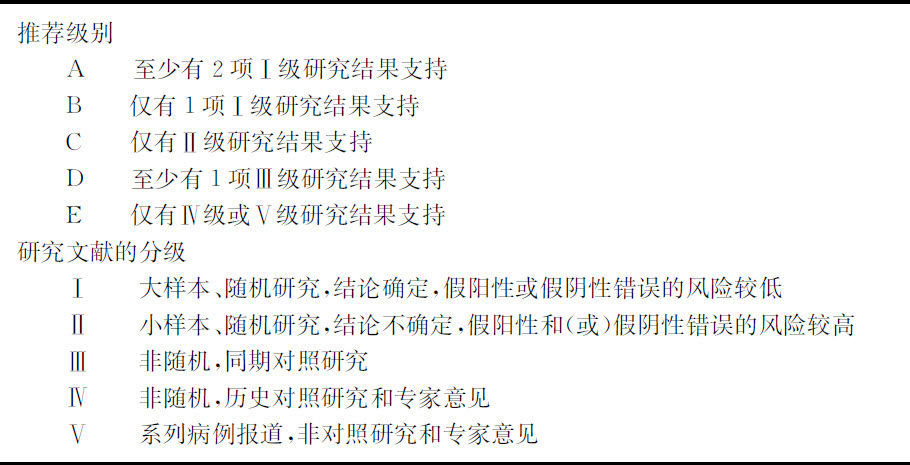
\includegraphics[width=\textwidth,height=\textheight,keepaspectratio]{./images/Image00300.jpg}
\end{longtable}

\section{ALI/ARDS的概念与流行病学}

ALI/ARDS是在严重感染、休克、创伤及烧伤等非心源性疾病过程中,肺毛细血管内皮细胞和肺泡上皮细胞损伤造成弥漫性肺间质及肺泡水肿,导致的急性低氧性呼吸功能不全或衰竭。以肺容积减少、肺顺应性降低、严重的通气/血流比例失调为病理生理特征,临床上表现为进行性低氧血症和呼吸窘迫,肺部影像学上表现为非均一性的渗出性病变。

流行病学调查显示ALI/ARDS是临床常见危重症。根据1994年欧美联席会议提出的ALI/ARDS诊断标准,ALI发病率为每年18/10万,ARDS为每年(13~23)/10万。2005年的研究显示,ALI/ARDS发病率分别在每年79/10万和59/10万。提示ALI/ARDS发病率显著增高,明显增加了社会和经济负担,这甚至可与胸部肿瘤、AIDS、哮喘或心肌梗死等相提并论。

多种危险因素可诱发ALI/ARDS,主要包括:①直接肺损伤因素。严重肺部感染,胃内容物吸入,肺挫伤,吸入有毒气体,淹溺、氧中毒等。②间接肺损伤因素。严重感染,严重的非胸部创伤,急性重症胰腺炎,大量输血,体外循环,弥漫性血管内凝血等。

病因不同,ARDS患病率也明显不同。严重感染时ALI/ARDS患病率可高达25%~50%,大量输血可达40%,多发性创伤达到11%~25%,而严重误吸时,ARDS患病率也可达9%~26%。同时存在两个或三个危险因素时,ALI/ARDS患病率进一步升高。另外,危险因素持续作用时间越长,ALI/ARDS的患病率越高,危险因素持续24、48及72小时时,ARDS患病率分别为76%、85%和93%。

虽然不同研究对ARDS病死率的报道差异较大,总体来说,目前ARDS的病死率仍较高。对1967~1994年国际正式发表的ARDS临床研究进行荟萃分析,3264例ARDS患者的病死率在50%左右。中国上海市15家成人ICU2001年3月至2002年3月ARDS病死率也高达68.5%。不同研究中ARDS的病因构成、疾病状态和治疗条件的不同可能是导致ARDS病死率不同的主要原因。

\section{ALI/ARDS病理生理与发病机制}

ALI/ARDS的基本病理生理改变是肺泡上皮和肺毛细血管内皮通透性增加所致的非心源性肺水肿。由于肺泡水肿、肺泡塌陷导致严重通气/血流比例失调,特别是肺内分流明显增加,从而产生严重的低氧血症。肺血管痉挛和肺微小血栓形成引发肺动脉高压。

ARDS早期的特征性表现为肺毛细血管内皮细胞与肺泡上皮细胞屏障的通透性增高,肺泡与肺间质内积聚大量的水肿液,其中富含蛋白及以中性粒细胞为主的多种炎症细胞。中性粒细胞粘附在受损的血管内皮细胞表面,进一步向间质和肺泡腔移行,释放大量促炎介质,如炎症性细胞因子、过氧化物、白三烯、蛋白酶、血小板活化因子等,参与中性粒细胞介导的肺损伤。除炎症细胞外,肺泡上皮细胞以及成纤维细胞也能产生多种细胞因子,从而加剧炎症反应过程。凝血和纤溶紊乱也参与ARDS的病程,ARDS早期促凝机制增强,而纤溶过程受到抑制,引起广泛血栓形成和纤维蛋白的大量沉积,导致血管堵塞以及微循环结构受损。ARDS早期在病理学上可见弥漫性肺损伤,透明膜形成及Ⅰ型肺泡上皮或内皮细胞坏死、水肿,Ⅱ型肺泡上皮细胞增生和间质纤维化等表现。

少数ALI/ARDS患者在发病第1周内可缓解,但多数患者在发病的5~7天后病情仍然进展,进入亚急性期。在ALI/ARDS的亚急性期,病理上可见肺间质和肺泡纤维化,Ⅱ型肺泡上皮细胞增生,部分微血管破坏并出现大量新生血管。部分患者呼吸衰竭持续超过14天,病理上常表现为严重的肺纤维化,肺泡结构破坏和重建。

\section{ALI/ARDS的临床特征与诊断}

一般认为,ALI/ARDS具有以下临床特征:①急性起病,在直接或间接肺损伤后12~48小时内发病;②常规吸氧后低氧血症难以纠正;③肺部体征无特异性,急性期双肺可闻及湿啰音或呼吸音减低;④早期病变以间质性为主,胸部X线片常无明显改变。病情进展后,可出现肺内实变,表现为双肺野普遍密度增高,透亮度减低,肺纹理增多、增粗,可见散在斑片状密度增高阴影,即弥漫性肺浸润影;⑤无心功能不全证据。

目前ALI/ARDS诊断仍广泛沿用1994年欧美联席会议提出的诊断标准:①急性起病;②氧合指数(PaO\textsubscript{2}
/FiO\textsubscript{2}
)≤200mmHg(不考虑呼气末正压水平);③正位X线胸片显示双肺均有斑片状阴影;④肺动脉嵌顿压≤18mmHg,或无左心房压力增高的临床证据。如PaO\textsubscript{2}
/FiO\textsubscript{2} ≤300mmHg且满足上述其他标准,则诊断为ALI。

\section{ALI/ARDS的治疗}

\subsubsection{原发病治疗}

全身性感染、创伤、休克、烧伤、急性重症胰腺炎等是导致ALI/ARDS的常见病因。严重感染患者有25%~50%发生ALI/ARDS,而且在感染、创伤等导致的多器官功能障碍综合征(MODS)中,肺往往也是最早发生衰竭的器官。目前认为,感染、创伤后的全身炎症反应是导致ARDS的根本原因。控制原发病,遏制其诱导的全身失控性炎症反应,是预防和治疗ALI/ARDS的必要措施。

推荐意见1:积极控制原发病是遏制ALI/ARDS发展的必要措施。(E级)

\subsubsection{呼吸支持治疗}

(1)氧疗 ALI/ARDS患者吸氧治疗的目的是改善低氧血症,使动脉血氧分压(PaO\textsubscript{2}
)达到60~80mmHg。可根据低氧血症改善的程度和治疗反应调整氧疗方式,首先使用鼻导管,当需要较高的吸氧浓度时,可采用可调节吸氧浓度的文丘里面罩或带储氧袋的非重吸式氧气面罩。ARDS患者往往低氧血症严重,大多数患者一旦诊断明确,常规的氧疗常常难以奏效,机械通气仍然是最主要的呼吸支持手段。

推荐意见2:氧疗是纠正ALI/ARDS患者低氧血症的基本手段。(E级)

(2)无创机械通气 无创机械通气(NIV)可以避免气管插管和气管切开引起的并发症,近年来得到了广泛的推广应用。尽管随机对照试验(RCT)证实NIV治疗慢性阻塞性肺疾病和心源性肺水肿导致的急性呼吸衰竭的疗效肯定,但是NIV在急性低氧性呼吸衰竭中的应用却存在很多争议。迄今为止,尚无足够的资料显示NIV可以作为ALI/ARDS导致的急性低氧性呼吸衰竭的常规治疗方法。

不同研究中NIV对急性低氧性呼吸衰竭的治疗效果差异较大,可能与导致低氧性呼吸衰竭的病因不同有关。2004年一项荟萃分析显示,在不包括慢性阻塞性肺疾病和心源性肺水肿的急性低氧性呼吸衰竭患者中,与标准氧疗相比,NIV可明显降低气管插管率,并有降低ICU住院时间及住院病死率的趋势。但分层分析显示NIV对ALI/ARDS的疗效并不明确。最近NIV治疗54例ALI/ARDS患者的临床研究显示,70%患者应用NIV治疗无效。逐步回归分析显示,休克、严重低氧血症和代谢性酸中毒是ARDS患者NIV治疗失败的预测指标。一项RCT研究显示,与标准氧疗比较,NIV虽然在应用第1小时明显改善ALI/ARDS患者的氧合,但不能降低气管插管率,也不改善患者预后。可见,ALI/ARDS患者应慎用NIV。

当ARDS患者神志清楚、血流动力学稳定,并能够得到严密监测和随时可行气管插管时,可以尝试NIV治疗。Sevransky等建议,在治疗全身性感染引起的ALI/ARDS时,如果预计患者的病情能够在48~72小时内缓解,可以考虑应用NIV。

应用NIV可使部分合并免疫抑制的ALI/ARDS患者避免有创机械通气,从而避免呼吸机相关性肺炎(VAP)的发生,并可能改善预后。目前两个小样本RCT研究和一个回顾性研究结果均提示,因免疫抑制导致的急性低氧性呼吸衰竭患者可以从NIV中获益。对40名实体器官移植的急性低氧性呼吸衰竭患者的RCT研究显示,与标准氧疗相比,NIV组气管插管率、严重并发症的发生率、入住ICU时间和ICU病死率明显降低,但住院病死率无差别。而对52名免疫抑制合并急性低氧性呼吸衰竭患者(主要是血液系统肿瘤)的RCT研究也显示,与常规治疗方案比较,NIV联合常规治疗方案可明显降低气管插管率,而且ICU病死率和住院病死率也明显减低。对237例机械通气的恶性肿瘤患者进行回顾性分析显示,NIV可以改善预后。因此,免疫功能低下的患者发生ALI/ARDS,早期可首先试用NIV。

一般认为,ALI/ARDS患者在以下情况时不适宜应用NIV:①神志不清;②血流动力学不稳定;③气道分泌物明显增加而且气道自洁能力不足;④因脸部畸形、创伤或手术等不能佩戴鼻面罩;⑤上消化道出血、剧烈呕吐、肠梗阻和近期食管及上腹部手术;⑥危及生命的低氧血症。应用NIV治疗ALI/ARDS时应严密监测患者的生命体征及治疗反应。如NIV治疗1~2小时后,低氧血症和全身情况得到改善,可继续应用NIV;若低氧血症不能改善或全身情况恶化,提示NIV治疗失败,应及时改为有创通气。

推荐意见3:预计病情能够短期缓解的早期ALI/ARDS患者可考虑应用无创机械通气。(C级)

推荐意见4:合并免疫功能低下的ALI/ARDS患者早期可首先试用无创机械通气。(C级)

推荐意见5:应用无创机械通气治疗ALI/ARDS应严密监测患者的生命体征及治疗反应。神志不清、休克、气道自洁能力障碍的ALI/ARDS患者不宜应用无创机械通气。(C级)

(3)有创机械通气

机械通气的时机选择 ARDS患者经高浓度吸氧仍不能改善低氧血症时,应气管插管进行有创机械通气。ARDS患者呼吸功明显增加,表现为严重的呼吸困难,早期气管插管机械通气可降低呼吸功,改善呼吸困难。虽然目前缺乏RCT研究评估早期气管插管对ARDS的治疗意义,但一般认为,气管插管和有创机械通气能更有效地改善低氧血症,降低呼吸功,缓解呼吸窘迫,并能够更有效地改善全身缺氧,防止肺外器官功能损害。

推荐意见6:ARDS患者应积极进行机械通气治疗。(E级)

肺保护性通气 由于ARDS患者大量肺泡塌陷,肺容积明显减少,常规或大潮气量通气易导致肺泡过度膨胀和气道平台压过高,加重肺及肺外器官的损伤。目前有5项多中心RCT研究比较了常规潮气量与小潮气量通气对ARDS病死率的影响。其中Amato和ARDSnet的研究显示,与常规潮气量通气组比较,小潮气量通气组ARDS患者病死率显著降低,另外3项研究应用小潮气量通气并不降低病死率。进一步分析显示,阴性结果的3项研究中常规潮气量组和小潮气量组的潮气量差别较小,可能是导致阴性结果的主要原因之一。

气道平台压能够客观反映肺泡内压,其过度升高可导致呼吸机相关肺损伤。在上述5项多中心RCT研究中,小潮气量组的气道平台压均<30cmH\textsubscript{2}
O,其中结论为小潮气量降低病死率的2项研究中,对照组气道平台压>30cmH\textsubscript{2}
O,而不降低病死率的3项研究中,对照组的气道平台压均<30cmH\textsubscript{2}
O。若按气道平台压分组(<23、23~27、27~33、>33cmH\textsubscript{2}
O),随气道平台压升高,病死率显著升高(\emph{P}
=0.002)。而以气道平台压进行调整,不同潮气量通气组(5~6、7~8、9~10、11~12ml/kg)病死率无显著差异(\emph{P}
=0.18),并随气道平台压升高,病死率显著增加(\emph{P}
<0.001)。说明在实施肺保护性通气策略时,限制气道平台压比限制潮气量更为重要。

由于ARDS肺容积明显减少,为限制气道平台压,有时不得不将潮气量降低,允许动脉血二氧化碳分压(PaCO\textsubscript{2}
)高于正常,即所谓的允许性高碳酸血症。允许性高碳酸血症是肺保护性通气策略的结果,并非ARDS的治疗目标。急性二氧化碳升高导致酸血症可产生一系列病理生理学改变,包括脑及外周血管扩张、心率加快、血压升高和心输出量增加等。但研究证实,实施肺保护性通气策略时一定程度的高碳酸血症是安全的。当然,颅内压增高是应用允许性高碳酸血症的禁忌证。酸血症往往限制了允许性高碳酸血症的应用,目前尚无明确的二氧化碳分压上限值,一般主张保持pH值>7.20,否则可考虑静脉输注碳酸氢钠。

推荐意见7:对ARDS患者实施机械通气时应采用肺保护性通气策略,气道平台压不应超过30~35cmH\textsubscript{2}
O。(B级)

肺复张 充分复张ARDS塌陷肺泡是纠正低氧血症和保证PEEP效应的重要手段。为限制气道平台压而被迫采取的小潮气量通气往往不利于ARDS塌陷肺泡的膨胀,而PEEP维持肺复张的效应依赖于吸气期肺泡的膨胀程度。目前临床常用的肺复张手法包括控制性肺膨胀、PEEP递增法及压力控制法(PCV法)。其中实施控制性肺膨胀采用恒压通气方式,推荐吸气压为30~45cmH\textsubscript{2}
O、持续时间30~40秒。临床研究证实肺复张手法能有效地促进塌陷肺泡复张,改善氧合,降低肺内分流。一项RCT研究显示,与常规潮气量通气比较,采用肺复张手法合并小潮气量通气,可明显改善ARDS患者的预后。然而,ARDSnet对肺复张手法的研究显示,肺复张手法并不能改善氧合,试验也因此而中断。有学者认为,得到阴性结果可能与复张的压力和时间不够有关。

肺复张手法的效应受多种因素影响。实施肺复张手法的压力和时间设定对肺复张的效应有明显影响,不同肺复张手法效应也不尽相同。另外,ARDS病因不同,对肺复张手法的反应也不同,一般认为,肺外源性的ARDS对肺复张手法的反应优于肺内源性的ARDS;ARDS病程也影响肺复张手法的效应,早期ARDS肺复张效果较好。

值得注意的是,肺复张手法可能影响患者的循环状态,实施过程中应密切监测。

推荐意见8:可采用肺复张手法促进ARDS患者塌陷肺泡复张,改善氧合。(E级)

PEEP的选择 ARDS广泛肺泡塌陷不但可导致顽固的低氧血症,而且部分可复张的肺泡周期性塌陷开放而产生剪切力,会导致或加重呼吸机相关肺损伤。充分复张塌陷肺泡后应用适当水平PEEP防止呼气末肺泡塌陷,改善低氧血症,并避免剪切力,防治呼吸机相关肺损伤。因此,ARDS应采用能防止肺泡塌陷的最低PEEP。

ARDS最佳PEEP的选择目前仍存在争议。通过荟萃分析比较不同PEEP对ARDS患者生存率的影响,结果表明,PEEP>12cmH\textsubscript{2}
O、尤其是PEEP>16cmH\textsubscript{2}
O时明显改善生存率。有学者建议可参照肺静态压力-容积(P-V)曲线低位转折点压力来选择PEEP。Amato及Villar的研究显示,在小潮气量通气的同时,以静态P-V曲线低位转折点压力+2cmH\textsubscript{2}
O作为PEEP,结果与常规通气相比ARDS患者的病死率明显降低。若有条件,应根据静态P-V曲线低位转折点压力+2cmH\textsubscript{2}
O来确定PEEP。

推荐意见9:应使用能防止肺泡塌陷的最低PEEP,有条件情况下,应根据静态P-V曲线低位转折点压力+2cmH\textsubscript{2}
O来确定PEEP。(C级)

自主呼吸 自主呼吸过程中膈肌主动收缩可增加ARDS患者肺重力依赖区的通气,改善通气血流比例失调,改善氧合。一项前瞻对照研究显示,与控制通气相比,保留自主呼吸的患者镇静剂使用量、机械通气时间和ICU住院时间均明显减少。因此,在循环功能稳定、人机协调性较好的情况下,ARDS患者机械通气时有必要保留自主呼吸。

推荐意见10:ARDS患者机械通气时应尽量保留自主呼吸。(C级)

半卧位 ARDS患者合并呼吸机相关性肺炎(VAP)往往使肺损伤进一步恶化,预防VAP具有重要的临床意义。机械通气患者平卧位易发生VAP。研究表明,由于气管插管或气管切开导致声门的关闭功能丧失,机械通气患者胃肠内容物易反流误吸进入下呼吸道,导致VAP。低于30°角的平卧位是院内获得性肺炎的独立危险因素。前瞻性RCT研究显示,机械通气患者平卧位和半卧位(头部抬高45°以上)VAP的患病率分别为34%和8%(\emph{P}
=0.003),经微生物培养确诊的VAP患病率分别为23%和5%(\emph{P}
=0.018)。可见,半卧位可显著降低机械通气患者VAP的发生。因此,除非有脊髓损伤等体位改变的禁忌证,机械通气患者均应保持半卧位,预防VAP的发生。

推荐意见11:若无禁忌证,机械通气的ARDS患者应采用30°~45°半卧位。(B级)

俯卧位通气 俯卧位通气通过降低胸腔内压力梯度、促进分泌物引流和促进肺内液体移动,明显改善氧合。一项随机研究采用每天7小时俯卧位通气,连续7天,结果表明俯卧位通气明显改善ARDS患者氧合,但对病死率无明显影响。然而,依据PaO\textsubscript{2}
/FiO\textsubscript{2} 对患者进行分层分析结果显示,PaO\textsubscript{2}
/FiO\textsubscript{2}
<88mmHg的患者俯卧位通气后病死率明显降低。此外,依据简化急性生理评分(SAPS)Ⅱ进行分层分析显示,SAPSⅡ高于49分的患者采用俯卧位通气后病死率显著降低。最近,另外一项每天20小时俯卧位通气的RCT研究显示,俯卧位通气有降低严重低氧血症患者病死率的趋势。可见,对于常规机械通气治疗无效的重度ARDS患者,可考虑采用俯卧位通气。

严重的低血压、室性心律失常、颜面部创伤及未处理的不稳定性骨折为俯卧位通气的相对禁忌证。当然,体位改变过程中可能发生如气管插管及中心静脉导管意外脱落等并发症,需要予以预防,但严重并发症并不常见。

推荐意见12:常规机械通气治疗无效的重度ARDS患者,若无禁忌证,可考虑采用俯卧位通气。(D级)

镇静镇痛与肌松 机械通气患者应考虑使用镇静镇痛剂,以缓解焦虑、躁动、疼痛,减少过度的氧耗。合适的镇静状态、适当的镇痛是保证患者安全和舒适的基本环节。

机械通气时应用镇静剂应先制定镇静方案,包括镇静目标和评估镇静效果的标准,根据镇静目标水平来调整镇静剂的剂量。临床研究中常用Ramsay评分来评估镇静深度、制定镇静计划,以Ramsay评分3~4分作为镇静目标。每天均需中断或减少镇静药物剂量直到患者清醒,以判断患者的镇静程度和意识状态。RCT研究显示,与持续镇静相比,每天间断镇静患者的机械通气时间、ICU住院时间和总住院时间均明显缩短,气管切开率、镇静剂的用量及医疗费用均有所下降。可见,对机械通气的ARDS患者应用镇静剂时应先制定镇静方案,并实施每日唤醒。

危重患者应用肌松药后,可能延长机械通气时间、导致肺泡塌陷和增加VAP发生率,并可能延长住院时间。机械通气的ARDS患者应尽量避免使用肌松药物。如确有必要使用肌松药物,应监测肌松水平以指导用药剂量,以预防膈肌功能不全和VAP的发生。

推荐意见13:对机械通气的ARDS患者,应制定镇静方案(镇静目标和评估)。(B级)

推荐意见14:对机械通气的ARDS患者,不推荐常规使用肌松剂。(E级)

(4)液体通气 部分液体通气是在常规机械通气的基础上经气管插管向肺内注入相当于功能残气量的全氟碳化合物,以降低肺泡表面张力,促进肺重力依赖区塌陷肺泡复张。研究显示,部分液体通气72小时后,ARDS患者肺顺应性可以得到改善,并且改善气体交换,对循环无明显影响。但患者预后均无明显改善,病死率仍高达50%左右。近期对90例ALI/ARDS患者的RCT研究显示,与常规机械通气相比,部分液体通气既不缩短机械通气时间,也不降低病死率,进一步分析显示,对于年龄<55岁的患者,部分液体通气有缩短机械通气时间的趋势。部分液体通气能改善ALI/ARDS患者气体交换,增加肺顺应性,可作为严重ARDS患者常规机械通气无效时的一种选择。

(5)体外膜氧合技术(ECMO) 建立体外循环后可减轻肺负担、有利于肺功能恢复。非对照临床研究提示,严重的ARDS患者应用ECMO后存活率为46%~66%。但RCT研究显示,ECMO并不改善ARDS患者预后。随着ECMO技术的改进,需要进一步的大规模研究结果来证实ECMO在ARDS治疗中的地位。

\subsubsection{ALI/ARDS药物治疗}

(1)液体管理 高通透性肺水肿是ALI/ARDS的病理生理特征,肺水肿的程度与ALI/ARDS的预后呈正相关,因此,通过积极的液体管理,改善ALI/ARDS患者的肺水肿具有重要的临床意义。

研究显示液体负平衡与感染性休克患者病死率的降低显著相关,且对于创伤导致的ALI/ARDS患者,液体正平衡使患者病死率明显增加。应用利尿剂减轻肺水肿可能改善肺部病理情况,缩短机械通气时间,进而减少呼吸机相关性肺炎等并发症的发生。但是利尿减轻肺水肿的过程可能会导致心输出量下降,器官灌注不足。因此,ALI/ARDS患者的液体管理必需考虑到二者的平衡,必须在保证脏器灌注前提下进行。

最近ARDS
net完成的不同ARDS液体管理策略的研究显示,尽管限制性液体管理与非限制性液体管理组病死率无明显差异,但与非限制性液体管理相比,限制性液体管理(利尿和限制补液)组患者第1周的液体平衡为负平衡(-136ml比+6992ml),氧合指数明显改善,肺损伤评分明显降低,而且ICU住院时间明显缩短。特别值得注意的是,限制性液体管理组的休克和低血压的发生率并无增加。可见,在维持循环稳定,保证器官灌注的前提下,限制性的液体管理策略对ALI/ARDS患者是有利的。

ARDS患者采用晶体还是胶体液进行液体复苏一直存在争论。最近的大规模RCT研究显示,应用白蛋白进行液体复苏,在改善生存率、脏器功能保护、机械通气时间及ICU住院时间等方面与生理盐水无明显差异。但值得注意的是,胶体渗透压是决定毛细血管渗出和肺水肿严重程度的重要因素。研究证实,低蛋白血症是严重感染患者发生ARDS的独立危险因素,而且低蛋白血症可导致ARDS病情进一步恶化,并使机械通气时间延长,病死率也明显增加。因此,对低蛋白血症的ARDS患者,有必要输入白蛋白或人工胶体,提高胶体渗透压。最近两个多中心RCT研究显示,对于存在低蛋白血症(血浆总蛋白<50~60g/L)的ALI/ARDS患者,与单纯应用呋塞米(速尿)相比,尽管白蛋白联合呋塞米治疗未能明显降低病死率,但可明显改善氧合、增加液体负平衡,并缩短休克时间。因此,对于存在低蛋白血症的ARDS患者,在补充白蛋白等胶体溶液的同时联合应用呋塞米,有助于实现液体负平衡,并改善氧合。人工胶体对ARDS是否也有类似的治疗效应,需进一步研究证实。

推荐意见15:在保证组织器官灌注前提下,应实施限制性的液体管理,有助于改善ALI/ARDS患者的氧合和肺损伤。(B级)

推荐意见16:存在低蛋白血症的ARDS患者,可通过补充白蛋白等胶体溶液和应用利尿剂,有助于实现液体负平衡,并改善氧合。(C级)

(2)糖皮质激素 全身和局部的炎症反应是ALI/ARDS发生和发展的重要机制,研究显示,血浆和肺泡灌洗液中的炎症因子浓度升高与ARDS病死率成正相关。长期以来,大量的研究试图应用糖皮质激素控制炎症反应,预防和治疗ARDS。早期的3项多中心RCT研究观察了大剂量糖皮质激素对ARDS的预防和早期治疗作用,结果糖皮质激素既不能预防ARDS的发生,对早期ARDS也没有治疗作用。但对于过敏原因导致的ARDS患者,早期应用糖皮质激素经验性治疗可能有效。此外,感染性休克并发ARDS的患者,如合并有肾上腺皮质功能不全,可考虑应用替代剂量的糖皮质激素。

持续的过度炎症反应和肺纤维化是导致ARDS晚期病情恶化和治疗困难的重要原因。糖皮质激素能抑制ARDS晚期持续存在的炎症反应,并能防止过度的胶原沉积,从而有可能对晚期ARDS有保护作用。小样本RCT试验显示,对于治疗1周后未好转的ARDS患者,糖皮质激素治疗组的病死率明显低于对照组,感染发生率与对照组无差异,高血糖发生率低于对照组。然而,最近ARDSnet的研究观察了糖皮质激素对晚期ARDS(患病7~24天)的治疗效应,结果显示糖皮质激素治疗(甲基泼尼松龙每天2mg/kg,分4次静脉点滴,14天后减量)并不降低60天病死率,但可明显改善低氧血症和肺顺应性,缩短患者的休克持续时间和机械通气时间。进一步亚组分析显示,ARDS发病>14天应用糖皮质激素会明显增加病死率。可见,对于晚期ARDS患者不宜常规应用糖皮质激素治疗。

推荐意见17:不推荐常规应用糖皮质激素预防和治疗ARDS。(B级)

(3)一氧化氮(NO)吸入 NO吸入可选择性扩张肺血管,而且NO分布于肺内通气良好的区域,可扩张该区域的肺血管,显著降低肺动脉压,减少肺内分流,改善通气血流比例失调,并且可减少肺水肿形成。临床研究显示,NO吸入可使约60%的ARDS患者氧合改善,同时肺动脉压、肺内分流明显下降,但对平均动脉压和心输出量无明显影响。但是氧合改善效果也仅限于开始NO吸入治疗的24~48小时内。两个RCT研究证实NO吸入并不能改善ARDS的病死率。因此,吸入NO不宜作为ARDS的常规治疗手段,仅在一般治疗无效的严重低氧血症时可考虑应用。

推荐意见18:不推荐吸入NO作为ARDS的常规治疗。(A级)

(4)肺泡表面活性物质 ARDS患者存在肺泡表面活性物质减少或功能丧失,易引起肺泡塌陷。肺泡表面活性物质能降低肺泡表面张力,减轻肺炎症反应,阻止氧自由基对细胞膜的氧化损伤。因此,补充肺泡表面活性物质可能成为ARDS的治疗手段。但是,早期的RCT研究显示,应用表面活性物质后,ARDS患者的血流动力学指标、动脉氧合、机械通气时间、ICU住院时间和30天生存率并无明显改善。有学者认为阴性结果可能与表面活性物质剂量不足有关。随后的小样本剂量对照研究显示,与安慰剂组及肺泡表面活性物质50mg/kg应用4次组比较,100mg/kg应用4次和8次,有降低ARDS28天病死率的趋势(43.8%、50%比18.8%、16.6%,\emph{P}
=0.075)。2004年有两个中心参加的RCT研究显示,补充肺泡表面活性物质能够短期内(24小时)改善ARDS患者的氧合,但并不影响机械通气时间和病死率。最近一项针对心脏手术后发生ARDS补充肺泡表面活性物质的临床研究显示,与既往病例比较,治疗组氧合明显改善,而且病死率下降。目前肺泡表面活性物质的应用仍存在许多尚未解决的问题,如最佳用药剂量、具体给药时间、给药间隔和药物来源等。因此,尽管早期补充肺表面活性物质,有助于改善氧合,还不能将其作为ARDS的常规治疗手段。有必要进一步研究,明确其对ARDS预后的影响。

(5)前列腺素E\textsubscript{1} 前列腺素E\textsubscript{1}
(PGE\textsubscript{1}
)不仅是血管活性药物,还具有免疫调节作用,可抑制巨噬细胞和中性粒细胞的活性,发挥抗炎作用。但是PGE\textsubscript{1}
没有组织特异性,静脉注射PGE\textsubscript{1}
会引起全身血管舒张,导致低血压。静脉注射PGE\textsubscript{1}
用于治疗ALI/ARDS,目前已经完成了多个RCT研究,但无论是持续静脉注射PGE\textsubscript{1}
,还是间断静脉注射脂质体PGE\textsubscript{1}
,与安慰剂组相比,PGE\textsubscript{1}
组在28天病死率、机械通气时间和氧合等方面并无益处。有研究认为吸入型PGE1可以改善氧合,但这需要进一步RCT研究证实。因此,只有在ALI/ARDS患者低氧血症难以纠正时,可以考虑吸入PGE\textsubscript{1}
治疗。

(6)N-乙酰半胱氨酸和丙半胱氨酸 抗氧化剂N-乙酰半胱氨酸(NAC)和丙半胱氨酸(Procysteine)通过提供合成谷胱甘肽(GSH)的前体物质半胱氨酸,提高细胞内GSH水平,依靠GSH氧化还原反应来清除体内氧自由基,从而减轻肺损伤。静脉注射NAC对ALI患者可以显著改善全身氧合和缩短机械通气时间。而近期在ARDS患者中进行的Ⅱ期临床试验证实,NAC有缩短肺损伤病程和阻止肺外器官衰竭的趋势,不能减少机械通气时间和降低病死率。丙半胱氨酸的Ⅱ、Ⅲ期临床试验也证实不能改善ARDS患者预后。因此,尚无足够证据支持NAC等抗氧化剂用于治疗ARDS。

(7)环氧化酶抑制剂 布洛芬等环氧化酶抑制剂,可抑制ALI/ARDS患者血栓素A\textsubscript{2}
的合成,对炎症反应有强烈抑制作用。小规模临床研究发现,布洛芬可改善全身性感染患者的氧合与呼吸力学。对严重感染的临床研究也发现布洛芬可以降低体温、减慢心率和减轻酸中毒,但是,亚组分析(ARDS患者130例)显示,布洛芬既不能降低危重患者ARDS的患病率,也不能改善ARDS患者30天生存率。因此,布洛芬等环氧化酶抑制剂尚不能用于ALI/ARDS常规治疗。

(8)细胞因子单克隆抗体或拮抗剂 炎症性细胞因子在ALI/ARDS发病中具有重要作用。动物实验应用单克隆抗体或拮抗剂中和肿瘤坏死因子(TNF)、白细胞介素(IL)-1和IL-8等细胞因子可明显减轻肺损伤,但多数临床试验获得阴性结果。近期结束的两项大样本临床试验,观察抗TNF单克隆抗体(Afelimomab)治疗严重感染的临床疗效,尤其是对于IL-6水平升高患者的疗效,但结果不一致。其中MONARCS研究(\emph{n}
=2634)显示,无论在IL-6高水平还是低水平的严重感染患者,Afelimomab治疗组的病死率明显降低。但另一项研究并不降低病死率。细胞因子单克隆抗体或拮抗剂是否能够用于ALI/ARDS的治疗,目前尚缺乏临床研究证据。因此,不推荐抗细胞因子单克隆抗体或拮抗剂用于ARDS治疗。

(9)己酮可可碱及其衍化物利索茶碱 己酮可可碱(Pentoxifylline)及其衍化物利索茶碱(Lisofylline)均可抑制中性粒细胞的趋化和激活,减少促炎因子TNFα、IL-1和IL-6等释放,利索茶碱还可抑制氧自由基释放。但目前尚无RCT试验证实己酮可可碱对ALI/ARDS的疗效。一项大样本的Ⅲ期临床试验(\emph{n}
=235)显示,与安慰剂组相比,应用利索茶碱治疗ARDS,28天病死率并无差异(利索茶碱31.9%,安慰剂24.7%,\emph{P}
=0.215),另外,28天内无需机械通气时间、无器官衰竭时间和院内感染发生率等亦无差异。因此,己酮可可碱或利索茶碱不推荐用于ARDS治疗。

(10)重组人活化蛋白C 重组人活化蛋白C(rhAPC或称Drotrecoginalfa)具有抗血栓、抗炎和纤溶特性,已被试用于治疗严重感染。Ⅲ期临床试验证实,持续静脉注射rhAPC每小时24μg/kg×96小时可以显著改善重度严重感染患者(APACHEⅡ>25)的预后。基于ARDS的本质是全身炎症反应,且凝血功能障碍在ARDS发生中具有重要地位,rhAPC有可能成为ARDS的治疗手段。但rhAPC治疗ARDS的Ⅱ期临床试验正在进行。因此,尚无证据表明rhAPC可用于ARDS治疗,当然,在严重感染导致的重度ARDS患者,如果没有禁忌证,可考虑应用rhAPC。rhAPC高昂的治疗费用也限制了它的临床应用。

(11)酮康唑 酮康唑是一种抗真菌药,但可抑制白三烯和血栓素A\textsubscript{2}
合成,同时还可抑制肺泡巨噬细胞释放促炎因子,有可能用于ARDS治疗。但是由ARDSnet完成的大样本(\emph{n}
=234)临床试验显示,酮康唑既不能降低ARDS的病死率,也不能缩短机械通气时间。在外科ICU患者中预防性口服酮康唑,治疗组的ARDS患病率明显降低,提示在高危患者中预防性应用酮康唑可能有效,但仍需要进一步临床试验证实。因此,目前仍没有证据支持酮康唑可用于ARDS常规治疗,同时为避免耐药,对于酮康唑的预防性应用也应慎重。

(12)鱼油 鱼油富含ω-3脂肪酸,如二十二碳六烯酸(DHA)、二十碳五烯酸(EPA)等,也具有免疫调节作用,可抑制二十烷花生酸样促炎因子释放,并促进PGE\textsubscript{1}
生成。研究显示,通过肠道给ARDS患者补充EPA、γ-亚油酸和抗氧化剂,可使患者肺泡灌洗液内中性粒细胞减少,IL-8释放受到抑制,病死率降低。对机械通气的ALI患者的研究也显示,肠内补充EPA和γ-亚油酸可以显著改善氧合和肺顺应性,明显缩短机械通气时间,但对生存率没有影响。新近的一项针对严重感染和感染性休克的临床研究显示,通过肠内营养补充EPA、γ-亚油酸和抗氧化剂,明显改善氧合,并可缩短机械通气时间与ICU住院时间,减少新发的器官功能衰竭,降低了28天病死率。此外,肠外补充EPA和γ-亚油酸也可缩短严重感染患者ICU住院时间,并有降低病死率的趋势。因此,对于ALI/ARDS患者,特别是严重感染导致的ARDS,可补充EPA和γ-亚油酸,以改善氧合,缩短机械通气时间。

推荐意见19:补充EPA和γ-亚油酸,有助于改善ALI/ARDS患者氧合,缩短机械通气时间。(C级)

\textbf{中华医学会重症医学分会}

《急性肺损伤/急性呼吸窘迫综合征诊断和治疗指南(2006)》工作组

组长:邱海波(东南大学附属中大医院)

组员(按姓氏笔画为序):马晓春(中国医科大学附属第一医院),王辰(首都医科大学朝阳医院),刘大为(中国医学科学院协和医院),邱海波(东南大学附属中大医院),秦英智(天津第三中心医院),席修明(首都医科大学附属北京复兴医院),黎毅敏(广州呼吸病研究所)

\protect\hypertarget{text00035.html}{}{}

\chapter{机械通气临床应用指南(2006)}

\textbf{中华医学会重症医学分会}

一、引言

二、危重症患者人工气道的选择

三、人工气道的管理

四、机械通气的目的和应用指征

五、无创正压通气(NPPV)

六、机械通气的基本模式

七、机械通气参数的调整(结合血流动力学与通气、氧合监护)

八、机械通气的并发症

九、呼吸机撤离

\section{引 言}

重症医学是研究危重病发生发展的规律,对危重病进行预防和治疗的临床学科。器官功能支持是重症医学临床实践的重要内容之一。机械通气从仅作为肺脏通气功能的支持治疗开始,经过多年来医学理论的发展及呼吸机技术的进步,已经成为涉及气体交换、呼吸做功、肺损伤、胸腔内器官压力及容积环境、循环功能等,可产生多方面影响的重要干预措施,并主要通过提高氧输送、肺脏保护、改善内环境等途径成为治疗多器官功能不全综合征的重要治疗手段。

机械通气不仅可以根据是否建立人工气道分为“有创”或“无创”,因为呼吸机具有的不同呼吸模式而使通气有众多的选择,不同的疾病对机械通气提出了具有特异性的要求,医学理论的发展及循证医学数据的增加使对呼吸机的临床应用更加趋于有明确的针对性和规范性。在这种条件下,不难看出,对危重患者的机械通气制定规范有明确的必要性。同时,多年临床工作的积累和多中心临床研究证据为机械通气指南的制定提供了越来越充分的条件。

中华医学会重症医学分会以循证医学的证据为基础,采用国际通用的方法,经过广泛征求意见和建议,反复认真讨论,达成关于机械通气临床应用方面的共识,以期对危重患者的机械通气的临床应用进行规范。重症医学分会今后还将根据医学证据的发展及新的共识对机械通气临床应用指南进行更新。

指南中的推荐意见依据2001年ISF提出的Delphi分级标准(表\ref{tabapp-3})。指南涉及的文献按照研究方法和结果分成5个层次,推荐意见的推荐级别按照Delphi分级分为A~E级,其中A级为最高。
 
\begin{longtable}{c}
  \caption{Delphi分级标准}
  \label{tabapp-3}
  \endfirsthead
  \caption[]{Delphi分级标准}
  \endhead
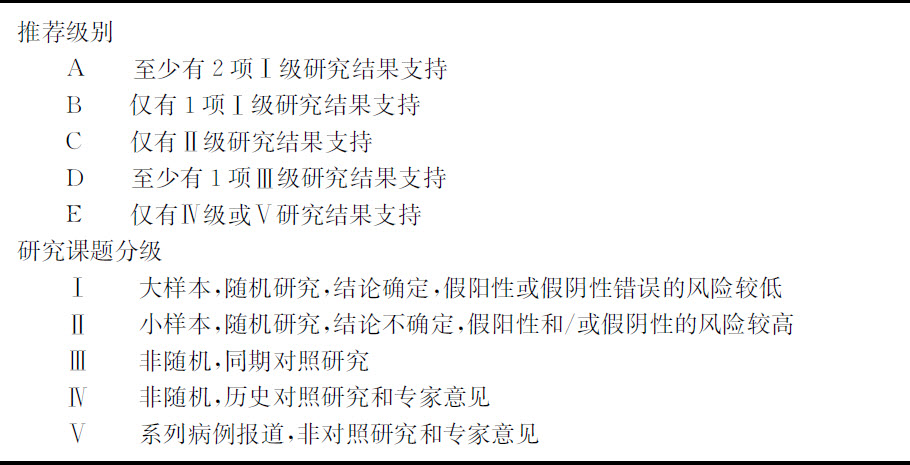
\includegraphics[width=\textwidth,height=\textheight,keepaspectratio]{./images/Image00301.jpg}
\end{longtable}

\section{危重症患者人工气道的选择}

人工气道是为了保证气道通畅而在生理气道与其他气源之间建立的连接,分为上人工气道和下人工气道,是呼吸系统危重症患者常见的抢救措施之一。上人工气道包括口咽气道和鼻咽气道,下人工气道包括气管插管和气管切开等。

建立人工气道的目的是保持患者气道的通畅,有助于呼吸道分泌物的清除及进行机械通气。人工气道的应用指征取决于患者呼吸、循环和中枢神经系统功能状况。结合患者的病情及治疗需要选择适当的人工气道。

\subsection{建立人工气道}

(1)经口气管插管 操作较易,插管的管径相对较大,便于气道内分泌物的清除,但影响会厌的功能,患者耐受性也较差。经口气管插管的关键在于暴露声门,在声门无法暴露的情况下,容易失败或出现并发症。

经口气管插管适应证:①严重低氧血症或高碳酸血症,或其他原因需较长时间机械通气,又不考虑气管切开;②不能自主清除上呼吸道分泌物、胃内反流物或出血,有误吸危险;③下呼吸道分泌物过多或出血,且清除能力较差;④存在上呼吸道损伤、狭窄、阻塞、气管食管瘘等严重影响正常呼吸;⑤患者突然出现呼吸停止,须紧急建立人工气道进行机械通气。

禁忌证或相对禁忌证包括:①张口困难或口腔空间小,无法经口插管;②无法后仰(如疑有颈椎骨折)。

(2)经鼻气管插管 较易固定,舒适性优于经口气管插管,患者较易耐受,但管径较小,导致呼吸功增加,不利于气道及鼻窦分泌物的引流。

经鼻气管插管适应证:除紧急抢救外,余同经口气管插管。

经鼻气管插管禁忌证或相对禁忌证:①紧急抢救,特别是院前急救;②严重鼻或颌面骨折;③凝血功能障碍;④鼻或鼻咽部梗阻,如鼻中隔偏曲、息肉、囊肿、脓肿、水肿、异物、血肿等;⑤颅底骨折。

与经口气管插管比较:经口气管插管减少了医院获得性鼻窦炎的发生,而医院获得性鼻窦炎与呼吸机相关性肺炎的发病有密切关系。因此,若短期内能脱离呼吸机的患者,应优先选择经口气管插管。但是,在经鼻气管插管技术操作熟练,或者患者不适于经口气管插管时,仍可以考虑先行经鼻气管插管。

(3)逆行气管插管术 指先行环甲膜穿刺,送入导丝,将导丝经喉至口咽部,由口腔或鼻腔引出,再将气管导管沿导丝插入气管。

逆行气管插管术适应证:因上呼吸道解剖因素或病理条件下,无法看到声带甚至会厌,无法完成经口或鼻气管插管。禁忌证:①甲状腺肿大,如甲亢或甲状腺癌等;②无法张口;③穿刺点肿瘤或感染;④严重凝血功能障碍;⑤不合作者。

上人工气道包括口咽通气道和鼻咽通气道,有助于保持上呼吸道的通畅。前者适用:舌后坠而导致上呼吸道梗阻,癫痫大发作或阵发性抽搐,以及经口气管插管时,可在气管插管旁插入口咽气道,防止患者咬闭气管插管发生部分梗阻或窒息。鼻咽通气道仅适用因舌后坠导致的上呼吸道阻塞,此时须注意凝血功能障碍者的鼻咽出血。

推荐意见1:机械通气患者建立人工气道可首选经口气管插管。(D级)

\subsection{气管切开的选择}

对于需要较长时间机械通气的患者,气管切开是常选择的人工气道方式。与其他人工气道比较,由于其管腔较大、导管较短,因而气道阻力及通气死腔较小,有利于气道分泌物的清除,减少呼吸机相关性肺炎的发生率。但是气管切开的时机仍有争议。1989年美国胸科医师协会建议:若预期机械通气时间在10天以内者优先选择气管插管,而超过21天者则优先选择气管切开术,在10至21天之间者则应每天对患者进行评估。这个建议并没有很强的研究结果支持,是建立在专家的经验之上。之后,有研究比较了“早期”和“晚期”气管切开,探讨“最佳”气管切开时机。研究发现,早期选择气管切开术,可以减少机械通气天数和ICU住院天数,减少呼吸机相关性肺炎的发生率,改善预后,这个观点尚需要大样本的RCT研究。对于“早期”的确切定义尚未统一,早至气管插管后48小时内,晚至气管插管后两周内,多数是在气管插管后7天或7天以内。目前,越来越多的研究倾向无需到21天后,2周内可考虑气管切开。

气管切开术适应证:①预期或需要较长时间机械通气治疗;②上呼吸道梗阻所致呼吸困难,如双侧声带麻痹、有颈部手术史、颈部放疗史;③反复误吸或下呼吸道分泌较多,患者气道清除能力差;④减少通气死腔,利于机械通气支持;⑤因喉部疾病致狭窄或阻塞无法气管插管;⑥头颈部大手术或严重创伤需行预防性气管切开,以保证呼吸道通畅;⑦高位颈椎损伤。气管切开术创伤较大,可发生切口出血或感染。

以下情况气管切开应慎重:①切开部位的感染或化脓;②切开部位肿物,如巨大甲状腺肿、气管肿瘤等;③严重凝血功能障碍,如弥漫性血管内凝血、特发性血小板减少症等。

经皮气管造口术(PCT)具有操作方法简单、快捷,手术创伤小等特点,临床研究表明,与气管切开术比较,有助于患者较早脱离呼吸机和减少ICU住院天数,以及减少并发症的发生率,但临床效果尚需进一步研究。

推荐意见2:短期内不能撤除人工气道的患者应尽早选择或更换为气管切开。(C级)

\section{人工气道的管理}

机械通气的患者应通过各种指标及时评估气道内是否有分泌物,包括听诊呼吸音,在容量控制机械通气时气道峰压是否增加,在压力控制机械通气时潮气量是否减少,患者是否不能进行有效地咳嗽,气道内可否见到分泌物等,应通过气道吸引确保分泌物的充分引流。

\subsection{气囊压的监测}

高容低压套囊压力在25~30cmH\textsubscript{2}
O之间既可有效封闭气道,又不高于气管黏膜毛细血管灌注压,可预防气道黏膜缺血性损伤及气管食管瘘,拔管后气管狭窄等并发症。Granja在一项95人的前瞻临床试验中得出结论,认为每天3次监测套囊压可预防气道黏膜缺血性损伤和气管狭窄。要注意气道压对套囊封闭压的影响,Guyton所做的一项15例患者的前瞻临床试验表明即使正确充盈套囊,如果气道峰压过高仍可造成气道黏膜缺血性损伤。高容低压套囊不需要间断放气。

推荐意见3:应常规监测人工气道的气囊压力。(C级)

\subsection{持续声门下吸引}

当使用带有侧孔的气管插管或气管切开套管时,可进行持续声门下吸引,以清除声门下至插管气囊之间的分泌物,又不损伤声带。在长期进行机械通气的患者中持续声门下吸引可延缓早发型呼吸机相关性肺炎的发生,降低其发生率。Kollef的一项以343例心脏外科患者为对象的研究表明在进行机械通气的患者中行持续声门下吸引可降低呼吸机相关性肺炎的发生率。另有多个临床随机对照实验表明持续声门下吸引可以降低并延缓通气机肺炎发生率,减少革兰阳性细菌及流感嗜血杆菌的感染。

推荐意见4:有条件的情况下,建立人工气道的患者应进行持续声门下吸引。(B级)

\subsection{气道湿化}

机械通气时的气道湿化包括主动湿化和被动湿化。主动湿化指在呼吸机管路内应用加热湿化器进行呼吸气体的加温加湿(包括不含加热导线,含吸气管路加热导线,含吸气呼气双管路加热导线);被动湿化指应用人工鼻(热湿交换器型)吸收患者呼出气的热量和水分进行吸入气体的加温加湿。不论何种湿化,都要求近端气道内的气体温度达到37℃,相对湿度100%,以维持气道黏膜完整,纤毛正常运动及气道分泌物的排出,降低呼吸道感染的发生。人工鼻(热湿交换器型)可较好进行加温加湿,与加热型湿化器相比不增加堵塞呼吸机管路发生率,并可保持远端呼吸机管路的清洁,因能增加气道阻力、死腔容积及吸气做功,故不推荐在慢性呼衰尤其在撤机困难的患者使用;Kirton曾报道人工鼻(热湿交换器型)较加热型湿化器能减少院内获得性肺炎的发生,近年来多个随机对照临床试验得出结论人工鼻(热湿交换器型)与加热型湿化器比较在呼吸机相关性肺炎的发生率上并无明显差异。有多个临床试验表明吸痰前滴入生理盐水进行气道湿化可使患者的血氧在吸痰后短期内明显下降,因此存在肺部感染的患者不推荐常规应用,可选择性应用痰液稀释。

推荐意见5:机械通气时应实施气道湿化。(C级)

\subsection{呼吸机管路的更换}

不应以控制感染为目的常规更换通气机管路。现有证据提示较长时间更换管路并不增加VAP的发生率,但关于管路使用的安全时间尚无定论。Graven等对24小时与48小时更换呼吸机管路进行比较,发现在吸气相气体培养或管道细菌定植培养均无差异。由Kollef和Hess等两个多中心随机对照研究提出:48小时与7天更换管路比较,每7天更换与不更换均没有增加VAP发病率且可明显降低医疗费用。国内也有类似报道比较7天与1天对VAP发生率的影响,一致认为频繁更换管路会增加VAP的发生率。虽然管路中冷凝水与VAP的关系缺乏证据,但应避免管路中聚积过多的冷凝水,更要避免过多的冷凝水流向患者气道或流入湿化罐,避免管路内被污染,一旦发现应及时清除。

推荐意见6:呼吸机管路不必频繁更换,一旦污染则应及时更换。(B级)

\section{机械通气的目的和应用指征}

\subsection{目的}

机械通气的生理学作用:提供一定水平的分钟通气量以改善肺泡通气;改善氧合;提供吸气末压(平台压)和呼气末正压(PEEP)以增加吸气末肺容积(EILV)和呼气末肺容积(EELV);对气道阻力较高和顺应性较低者,机械通气可降低呼吸功耗,缓解呼吸肌疲劳。因此,应用机械通气可达到以下临床目的。

(1)纠正急性呼吸性酸中毒 通过改善肺泡通气使动脉血二氧化碳分压和pH值得以改善。通常应使动脉血二氧化碳分压和pH值维持在正常水平。对于慢性呼吸衰竭急性加重者(如COPD)应达到缓解期水平。对存在气压伤较高风险的患者,应适当控制气道压水平。

(2)纠正低氧血症 通过改善肺泡通气、提高吸入氧浓度、增加肺容积和减少呼吸功耗等手段以纠正低氧血症。机械通气改善氧合的基本目标是动脉血氧分压>60mmHg或SaO\textsubscript{2}
>90%。动脉氧含量(CaO\textsubscript{2}
)与动脉血氧分压和血红蛋白(HB)有关,而氧输送量(DO\textsubscript{2}
)不但与CaO\textsubscript{2}
有关,还与心输出量有关,因此,为了改善组织缺氧应考虑上述因素对DO\textsubscript{2}
的影响。

(3)降低呼吸功耗,缓解呼吸肌疲劳 由于气道阻力增加、呼吸系统顺应性降低和内源性呼气末正压(PEEPi)的出现,呼吸功耗显著增加,严重者出现呼吸肌疲劳。对这类患者适时地使用机械通气可以减少呼吸肌做功,达到缓解呼吸肌疲劳的目的。

(4)防止肺不张 对于可能出现肺膨胀不全的患者(如术后胸腹活动受限、神经肌肉疾病等),机械通气可通过增加肺容积而预防和治疗肺不张。

(5)为安全使用镇静和肌松剂提供通气保障 对于需要抑制或完全消除自主呼吸的患者,如接受手术或某些特殊操作者,呼吸机可为使用镇静和肌松剂提供通气保障。

(6)稳定胸壁 在某些情况下(如肺叶切除、连枷胸等),由于胸壁完整性受到破坏,通气功能严重受损,此时机械通气可通过机械性的扩张使胸壁稳定,以保证充分的通气。

\subsection{应用指征}

在出现较为严重的呼吸功能障碍时,应使用机械通气。如果延迟实施机械通气,患者因严重低氧和CO\textsubscript{2}
潴留而出现多脏器功能受损,机械通气的疗效显著降低。因此,机械通气宜早实施。符合下述条件应实施机械通气:经积极治疗后病情仍继续恶化;意识障碍;呼吸形式严重异常,如呼吸频率>35~40次/分或<6~8次/分,呼吸节律异常,自主呼吸微弱或消失;血气分析提示严重通气和/或氧合障碍:动脉血氧分压<50mmHg,尤其是充分氧疗后仍<50mmHg;动脉血二氧化碳分压进行性升高,pH值动态下降。

下述情况机械通气时可能使病情加重:如气胸及纵隔气肿未行引流,肺大疱和肺囊肿,低血容量性休克未补充血容量,严重肺出血,气管食管瘘等。但在出现致命性通气和氧合障碍时,应积极处理原发病(如尽快行胸腔闭式引流,积极补充血容量等),同时不失时机地应用机械通气。

\section{无创正压通气(NPPV)}

NPPV是指无需建立人工气道的正压通气,常通过鼻/面罩等方法连接患者。临床研究证明,在某些病例NPPV可以减少急性呼吸衰竭的气管插管或气管切开及相应的并发症,改善预后;减少慢性呼吸衰竭呼吸机的依赖,减少患者的痛苦和医疗费用,提高生活的质量。

NPPV可以避免人工气道的不良反应和并发症(气道损伤、呼吸机相关性肺炎等),同时也不具有人工气道的一些作用(如气道引流、良好的气道密封性等)。由于NPPV不可避免地存在或多或少的漏气,使得通气支持不能达到与IMV相同的水平,临床主要应用于意识状态较好的轻、中度的呼吸衰竭,或自主呼吸功能有所恢复、从IMV撤离的呼吸衰竭患者;而有意识障碍、有并发症或多器官功能损害的严重呼吸衰竭宜选择IMV。NPPV与IMV各自具有不同的适应证和临床地位,两者相互补充,而不是相互替代。

\subsection{适应证和禁忌证}

适应证:患者出现较为严重的呼吸困难,动用辅助呼吸肌,常规氧疗方法(鼻导管和面罩)不能维持氧合或氧合障碍有恶化趋势时,应及时使用NPPV。但患者必须具备使用NPPV的基本条件:较好的意识状态、咯痰能力、自主呼吸能力、血流动力学稳定和良好的配合NPPV的能力。

禁忌证:意识障碍,呼吸微弱或停止,无力排痰,严重的脏器功能不全(上消化道大出血、血流动力学不稳定等),未经引流的气胸或纵隔气肿,严重腹胀,上气道或颌面部损伤/术后/畸形,不能配合NPPV或面罩不适等。

\subsection{临床应用}

Girault等人总结2年应用NPPV的临床实践表明:64%的急性呼吸衰竭患者避免了气管插管,而NPPV失败后改用有创通气者,其死亡率仅为10.5%,因此NPPV可作为临床治疗急性呼吸衰竭的一线选择。但对于不同类型的急性呼吸衰竭,NPPV使用的支持证据不同。对于急性加重期COPD(慢性阻塞性肺疾病急性加重期)、急性心源性肺水肿和免疫抑制患者,已有较多的RCT研究表明,较早地应用NPPV可降低这类患者的气管插管率和住院病死率。对于支气管哮喘持续状态、术后可能发生呼吸衰竭和拒绝插管者,仅有为数不多的研究表明NPPV可能对这些患者有效,部分患者有避免气管插管的可能,证据尚不充分,临床可以试用,不作为一线治疗手段。而对于肺炎和和ARDS,目前支持证据很有限,对于病情相对较轻者才可试验性使用,但须严密观察,一旦病情恶化,立即采取气管插管行有创通气治疗,以免延误病情。

推荐意见7:NPPV可作为急性加重期COPD和急性心源性肺水肿患者的一线治疗手段。(A级)

推荐意见8:合并免疫抑制的呼吸衰竭患者可首先试用NPPV。(B级)

\subsection{呼吸机的选择}

要求能提供双水平正压通气模式,提供的吸气压力可达到20~30cmH\textsubscript{2}
O,能满足患者吸气需求的高流量气体(>100L/分),具备一些基本的报警功能;若用于I型呼吸衰竭,要求能提供较高的吸氧浓度(>50%)和更高的流速需求。

\subsection{连接方式}

应准备不同大小型号的鼻罩和口鼻面罩以供不同患者使用。鼻罩和口鼻面罩都能成功地用于急性呼吸衰竭的患者,在应用NPPV的初始阶段,口鼻面罩应首先考虑应用,患者病情改善24小时后还需较长时间应用者,NPPV可更换为鼻罩。

\subsection{通气模式与参数调节}

持续气道内正压和双水平正压通气是最常用的两种通气模式,后者最为常用。双水平正压通气有两种工作方式:自主呼吸通气模式(S模式,相当于PSV+PEEP)和后备控制通气模式(T模式,相当于PCV+PEEP)。因此,BiPAP的参数设置包括吸气压(IPAP),呼气压(EPAP)及后备控制通气频率。当自主呼吸间隔时间低于设定值(由后备频率决定)时,即处于S模式;自主呼吸间隔时间超过设定值时,即由S模式转向T模式,即启动时间切换的背景通气PCV。在ACPE患者首选CPAP,如果存在高碳酸血症或呼吸困难不缓解可考虑换用BiPAP。

BiPAP参数调节原则:IPAP/EPAP均从较低水平开始,患者耐受后再逐渐上调,直到达满意的通气和氧合水平,或调至患者可能耐受的水平。BiPAP模式通气参数设置的常用参考值如下表所示。


\begin{longtable}{c}
  \caption{双水平正压通气模式参数设置常用参考值}
  \label{tabapp-4}
  \endfirsthead
  \caption[]{双水平正压通气模式参数设置常用参考值}
  \endhead
\centering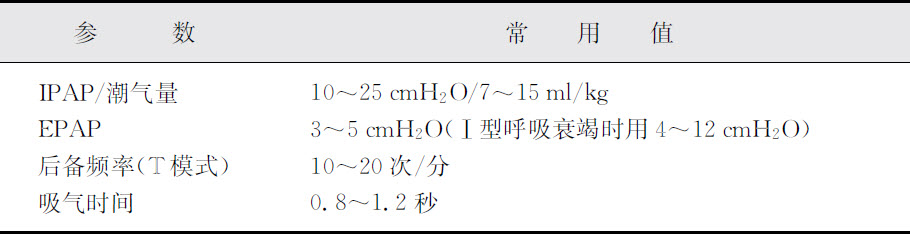
\includegraphics[width=\textwidth,height=\textheight,keepaspectratio]{./images/Image00302.jpg}
\end{longtable}

\subsection{NPPV转换为有创通气的时机}

在应用NPPV过程中如何及时、准确地判断NPPV的效果,对于是继续应用NPPV,还是转换为IMV具有重要意义:一方面可以提高NPPV的有效性,又可避免延迟气管插管,从而提高NPPV的安全性。对于能够成功应用NPPV的患者的特征是:基础病情较轻,应用NPPV后血气能快速明显改善,呼吸频率下降。可能失败的相关因素为:较高的APACHEⅡ评分、意识障碍或昏迷、对NPPV的初始治疗反应不明显、胸片提示肺炎、呼吸道分泌物很多、高龄、满口缺齿、营养不良等。

推荐意见9:应用NPPV1~2小时(短期)病情不能改善应转为有创通气。(推荐级别D级)

\section{机械通气的基本模式}

\subsection{分类}

(1)“定容”型通气和“定压”型通气

①定容型通气:呼吸机以预设通气容量来管理通气,即呼吸机送气达预设容量后停止送气,依靠肺、胸廓的弹性回缩力被动呼气。

常见的定容通气模式有容量控制通气、容量辅助控制通气、间歇指令通气(IMV)和同步间歇指令通气(SIMV)等,也可将它们统称为容量预设型通气(volume
preset ventilation,VPV)。

VPV能够保证潮气量的恒定,从而保障分钟通气量;VPV的吸气流速波形为恒流波形,即方波,不能适应患者的吸气需要,尤其存在自主呼吸的患者,这种人机的不协调增加镇静剂和肌松剂的需要,并消耗很高的吸气功,从而诱发呼吸肌疲劳和呼吸困难;当肺顺应性较差或气道阻力增加时,使气道压过高。

②定压型通气:呼吸机以预设气道压力来管理通气,即呼吸机送气达预设压力且吸气相维持该压力水平,而潮气量是由气道压力与PEEP之差及吸气时间决定,并受呼吸系统顺应性和气道阻力的影响。

常见的定压型通气模式有压力控制通气(PCV)、压力辅助控制通气(P-ACV)、压力控制同步间歇指令通气(PC-SIMV)、压力支持通气(PSV)等,统称为压力预设型通气(pressure
preset ventilation,PPV)。

PPV时潮气量随肺顺应性和气道阻力而改变;气道压力一般不会超过预置水平,利于限制过高的肺泡压和预防VILI;流速多为减速波,肺泡在吸气早期即充盈,利于肺内气体交换。

(2)控制通气和辅助通气

①控制通气(controlled
ventilation,CV):呼吸机完全代替患者的自主呼吸,呼吸频率、潮气量、吸呼比、吸气流速,呼吸机提供全部的呼吸功。

CV适用于严重呼吸抑制或伴呼吸暂停的患者,如麻醉、中枢神经系统功能障碍、神经肌肉疾病、药物过量等情况。在CV时可对患者呼吸力学进行监测,如静态肺顺应性、内源性PEEP、阻力等肺机械参数。

CV参数设置不当,可造成通气不足或过度通气;应用镇静剂或肌松剂将导致分泌物清除障碍等;长时间应用CV将导致呼吸肌萎缩或呼吸机依赖。故应用CV时应明确治疗目标和治疗终点,对一般的急性或慢性呼吸衰竭,只要患者条件许可宜尽早采用“辅助通气支持”。

②辅助通气(assisted
ventilation,AV)依靠患者的吸气努力触发呼吸机吸气活瓣实现通气,当存在自主呼吸时,根据气道内压力降低(压力触发)或气流(流速触发)的变化触发呼吸机送气,按预设的潮气量(定容)或吸气压力(定压)输送气体,呼吸功由患者和呼吸机共同完成。

AV适用于呼吸中枢驱动正常的患者,通气时可减少或避免应用镇静剂,保留自主呼吸以减轻呼吸肌萎缩,改善机械通气对血流动力学的影响,利于撤机过程。

\subsection{常用模式}

(1)辅助控制通气 辅助控制通气(assist-control
ventilation,ACV)是辅助通气(AV)和控制通气(CV)两种模式的结合,当患者自主呼吸频率低于预置频率或患者吸气努力不能触发呼吸机送气时,呼吸机即以预置的潮气量及通气频率进行正压通气,即CV;当患者的吸气能触发呼吸机时,以高于预置频率进行通气,即AV。ACV又分为压力辅助控制通气(P-ACV)和容量辅助控制通气(V-ACV)。

参数设置:容量切换A-C:触发敏感度、潮气量、通气频率、吸气流速/流速波形;压力切换A-C:触发敏感度、压力水平、吸气时间、通气频率。

特点:A-C为ICU患者机械通气的常用模式,通过设定的呼吸频率及潮气量(或压力),提供通气支持,使患者的呼吸肌得到的休息,CV确保最低的分钟通气量。随病情好转,逐步降低设置条件,允许患者自主呼吸,呼吸功由呼吸机和患者共同完成,呼吸机可与自主呼吸同步。

(2)同步间歇指令通气 同步间歇指令通气(synchronized intermittent
mandatory
ventilation,SIMV)是自主呼吸与控制通气相结合的呼吸模式,在触发窗内患者可触发和自主呼吸同步的指令正压通气,在两次指令通气之间触发窗外允许患者自主呼吸,指令呼吸是以预设容量(容量控制SIMV)或预设压力(压力控制SIMV)的形式送气。

参数设置:潮气量、流速/吸气时间、控制频率、触发敏感度,当压力控制SIMV时需设置压力水平。

特点:通过设定IMV的频率和潮气量确保最低分钟量;SIMV能与患者的自主呼吸同步,减少患者与呼吸机的对抗,减低正压通气的血流动力学影响;通过调整预设的IMV的频率改变呼吸支持的水平,即从完全支持到部分支持,减轻呼吸肌萎缩;用于长期带机的患者的撤机;但不适当的参数设置(如流速及V\textsubscript{T}
设定不当)可增加呼吸功,导致呼吸肌疲劳或过度通气。

容量通气方式临床应用:容量方式保证潮气量,适当的流速设定影响V\textsubscript{T}
及气道压的变化,其触发方式可为流速或压力触发,近年研究表明:流速触发比压力触发可以明显减轻呼吸功。呼吸机送气流速波形依据肺病变不同(即阻力、顺应性)可采用恒流或减速波方式送气,以利于肺内气体分布改善氧合。该类模式又将压力限制或容量限制整合到模式中去,明显减轻压力伤与容积伤的危险。控制通气与自主呼吸相结合方式有利于循序渐进增大自主呼吸,在此期间可与PSV和用,使患者容易过渡到自主呼吸,因此可作为撤机方式之一。在ARDS患者应用容量模式时,PEEP设定应注意调整潮气量以避免超过平台压加重肺损伤。当前,应用容量通气模式时,只要参数调节适当可明显减轻或克服传统容量模式许多不利因素,已成为当前ICU常用的呼吸支持的方式之一。

(3)压力支持通气 压力支持通气(pressure support
ventilation,PSV)属部分通气支持模式,是由患者触发、压力目标、流量切换的一种机械通气模式,即患者触发通气,呼吸频率,潮气量及吸呼比,当气道压力达预设的压力支持水平时,吸气流速降低至某一阈值水平以下时,由吸气切换到呼气。

参数设置:压力、触发敏感度,有些呼吸机有压力上升速度、呼气灵敏度(E\textsubscript{SENS}
)。

临床应用:适用于完整的呼吸驱动能力的患者,当设定水平适当时,则少有人机对抗,减轻呼吸功;PSV是自主呼吸模式,支持适当可减轻呼吸肌的废用性萎缩;对血流动力学影响较小,包括心脏外科手术后患者;一些研究认为5~8cmH\textsubscript{2}
O的PSV可克服气管导管和呼吸机回路的阻力,故PSV可应用于呼吸机的撤离;当出现浅快呼吸患者,应调整PS水平以改善人机不同步;当管路有大量气体泄露,可引起持续吸气压力辅助,呼吸机就不能切换到呼气相。对呼吸中枢驱动功能障碍的患者也可导致每分通气量的变化,甚至呼吸暂停而窒息,因此不宜使用该模式。

(4)持续气道内正压 持续气道内正压(continuous positive airway
pressure,CPAP)是在自主呼吸条件下,整个呼吸周期以内(吸气及呼气期间)气道均保持正压,患者完成全部的呼吸功,是呼气末正压(PEEP)在自主呼吸条件下的特殊技术。

参数设置:仅需设定CPAP水平。

临床应用:适用于通气功能正常的低氧患者,CPAP具有PEEP的各种优点和作用,如增加肺泡内压和功能残气量,增加氧合,防止气道和肺泡的萎陷,改善肺顺应性,降低呼吸功,对抗内源性PEEP;设定CPAP应根据PEEPi和血流动力学的变化,CPAP过高增加气道压,减少回心血量,对心功能不全的患者血流动力学产生不利影响。但在CPAP时由于自主呼吸可使胸内压较相同PEEP时略低。

(5)双相气道正压通气 双相气道正压通气(biphasic positive airway
pressure,BIPAP)是指给予两种不同水平的气道正压,为高压力水平(P\textsubscript{high}
)和低压力水平(P\textsubscript{low}
)之间定时切换,且其高压时间、低压时间、高压水平、低压水平各自可调,从P\textsubscript{high}
转换至P\textsubscript{low}
时,增加呼出气量,改善肺泡通气。该模式允许患者在两种水平上呼吸,可与PSV合用以减轻患者呼吸功。

参数设置:高压水平(P\textsubscript{high}
)、低压水平(P\textsubscript{low}
)即PEEP、高压时间(T\textsubscript{insp} )、呼吸频率、触发敏感度。

临床应用:BIPAP通气时气道压力周期性地在高压水平和低压水平之间转换,每个压力水平,压力时间均可独立调节,可转化为反比BIPAP或气道压力释放通气(APRV);BIPAP通气时患者的自主呼吸少受干扰,当高压时间持续较长时,增加平均气道压,可明显改善患者的氧合;BIPAP通气时可由控制通气向自主呼吸过度,不用变更通气模式直至呼吸机撤离。该模式具有压力控制模式特点,但在高压水平又允许患者自主呼吸;与PSV合用时,患者容易从控制呼吸向自主呼吸过渡。因此,该模式既适用于氧合障碍型呼吸衰竭,亦适用于通气障碍型呼吸衰竭。

(6)其他模式

①高频振荡通气(HFOV)

高频振荡通气(HFOV)是目前所有高频通气中频率最高的一种,可达15~17Hz。由于频率高,每次潮气量接近或小于解剖死腔。其主动的呼气原理(即呼气时系统呈负压,将气体抽吸出体外),保证了二氧化碳的排出,侧支气流供应使气体充分湿化。HFOV通过提高肺容积、减少吸呼相的压差、降低肺泡压(仅为常规正压通气的1/5~1/15)、避免高浓度吸氧等以改善氧合及减少肺损伤,是目前先进的高频通气技术。

应用指征:主要用于重症ARDS患者:FiO\textsubscript{2}
>0.6时PaO\textsubscript{2} /FiO\textsubscript{2}
<200持续>24小时,并且平均气道压(MAP)>20cmH\textsubscript{2}
O(或PEEP>15cmH\textsubscript{2}
O),或氧合指数>20(氧合指数=平均气道压×吸入氧浓度×100/氧分压)。

参数设置:

平均气道压(MAP):为基础气道压,其大小与动脉血氧分压关系最为密切。初始设置:高于常规通气MAP2~4cmH\textsubscript{2}
O,之后根据氧合和血流动力学调节,最高不超过45cmH\textsubscript{2} O。

FiO\textsubscript{2} 设置:与MAP配合,尽量使FiO\textsubscript{2}
<60%。

压力变化幅度(ΔP):每次振荡所产生的压力变化,与动脉血二氧化碳分压水平密切相关。初始设置:50~70cmH\textsubscript{2}
O,之后根据动脉血二氧化碳分压或胸廓振荡幅度调节。

频率:3~6Hz。降低频率有助于降低动脉血二氧化碳分压。

吸气时间占呼吸周期(I/E):33%~50%。增加I/E有助于降低动脉血二氧化碳分压和改善氧合。

偏向气流(bias flow):40~60L/分。

气囊漏气:有助于降低动脉血二氧化碳分压。

肺复张法(RM)的应用:联合应用RM可进一步改善氧合。

临床应用定位:

成人ARDS的RCT研究显示,HFOV在改善氧合方面较常规通气有一定优势,病死率有降低趋势(52%vs37%),但血流动力学指标及气压伤发生率无显著性差异。因此,HFOV应视为具有与常规通气具有相同疗效和安全性的一种呼吸支持手段,早期应用可能效果更好。

②成比例辅助通气

成比例辅助通气(proportional assist
ventilation,PAV)是一种部分通气支持,呼吸机送气与患者呼吸用力成比例,PAV的目标是让患者舒适地获得由自身任意支配的呼吸形式和通气水平。

参数设置:流速辅助(FA)、容量辅助(VA)、持续气道内正压(CPAP)。

临床应用:呼吸负荷主要包括弹性负荷和阻力负荷,PAV模式下呼吸机提供的补偿是针对弹性负荷和阻力负荷,与PSV相比呼吸机能更好地与患者配合,该通气方式下的流速时间波形为接近生理状态的正弦波,研究显示与其他通气模式比较相同通气参数时平均气道压较低,对血流动力学影响较小,尤其适用于心功能低下的撤机困难患者;在PAV模式下,当患者吸气努力较小时,压力支持水平也较低,当吸气努力较大时,压力支持水平也较高,通过调节FA、VA循序渐进地增大自主呼吸,锻炼呼吸肌以适应通气需要,避免患者呼吸机依赖。该模式可作为困难撤机患者的撤机方式,尤其适用于呼吸机依赖的患者。通过持续气道内正压(CPAP)克服内源性PEEP(PEEPi),使吸气功耗减低。

\section{氧合监护)}

\subsection{潮气量的设定}

在容量控制通气模式下,潮气量的选择应保证足够的气体交换及患者的舒适性,通常依据体重选择5~12ml/kg,并结合呼吸系统的顺应性、阻力进行调整,避免气道平台压超过30~35cmH\textsubscript{2}
O。在压力控制通气模式时,潮气量主要由预设的压力、吸气时间、呼吸系统的阻力及顺应性决定;最终应根据动脉血气分析进行调整。

\subsection{呼吸频率的设定}

呼吸频率的选择根据分钟通气量及目标PCO\textsubscript{2}
水平,成人通常设定为12~20次/分,急/慢性限制性肺疾病时也可根据分钟通气量和目标PCO\textsubscript{2}
水平超过20次/分,准确调整呼吸频率应依据动脉血气分析的变化综合调整VT与f。

\subsection{流速调节}

理想的峰流速应能满足患者吸气峰流速的需要,成人常用的流速设置在40~60L/分之间,根据分钟通气量和呼吸系统的阻力和肺的顺应性调整,流速波形在临床常用减速波或方波。压力控制通气时流速由选择的压力水平、气道阻力及受患者的吸气努力影响。

\subsection{吸气时间/I:E设置}

I:E的选择是基于患者的自主呼吸水平、氧合状态及血流动力学,适当的设置能保持良好的人机同步性,机械通气患者通常设置吸气时间为0.8~1.2秒或吸呼比为1∶1.5~2;控制通气患者,为抬高平均气道压改善氧合可适当延长吸气时间及吸呼比,但应注意患者的舒适度、监测PEEPi及对心血管系统的影响。

\subsection{触发灵敏度调节}

一般情况下,压力触发常为-0.5~-1.5cmH\textsubscript{2}
O,流速触发常为2~5L/分,合适的触发灵敏度设置将明显使患者更舒适,促进人机协调;一些研究表明流速触发较压力触发能明显减低患者呼吸功;若触发敏感度过高,会引起与患者用力无关的误触发,若设置触发敏感度过低,将显著增加患者的吸气负荷,消耗额外呼吸功。

\subsection{吸入氧浓度(FiO2 )}

机械通气初始阶段,可给高FiO\textsubscript{2}
(100%)以迅速纠正严重缺氧,以后依据目标动脉血氧分压、PEEP水平、MAP水平和血流动力学状态,酌情降低FiO\textsubscript{2}
至50%以下,并设法维持SaO\textsubscript{2}
>90%,若不能达上述目标,即可加用PEEP、增加平均气道压,应用镇静剂或肌松剂;若适当PEEP和MAP可以使SaO\textsubscript{2}
>90%,应保持最低的FiO\textsubscript{2} 。

\subsection{PEEP的设定}

设置PEEP的作用是使萎陷的肺泡复张、增加平均气道压、改善氧合,同时影响回心血量,及左室后负荷,克服PEEPi引起呼吸功的增加。PEEP常应用于以ARDS为代表的I型呼吸衰竭,PEEP的设置在参照目标动脉血氧分压和氧输送的基础上,与FiO\textsubscript{2}
与V\textsubscript{T}
联合考虑,虽然PEEP设置的上限没有共识,但下限通常在P-V曲线的低拐点(LIP)或LIP之上2cmH\textsubscript{2}
O;还可根据PEEPi指导PEEP的调节,外源性PEEP水平大约为PEEPi的80%,以不增加总PEEP为原则。

\section{机械通气的并发症}

机械通气是重要的生命支持手段之一,但机械通气也会带来一些并发症,甚至是致命的。合理应用机械通气将有助于减少甚至避免并发症的产生。因此,了解机械通气的并发症,具有重要的临床意义。

\subsection{气管插管相关的并发症}

人工气道是经口/经鼻插入或经气管切开处插入气管所建立的气体通道。临床上常用的人工气道是气管插管和气管切开。

(1)导管易位

插管过深或固定不佳,均可使导管进入支气管。因右主支气管与气管所成角度较小,插管过深进入右主支气管,可造成左侧肺不张及同侧气胸。插管后应立即听诊双肺,如一侧肺呼吸减弱并叩浊提示肺不张,呼吸音减低伴叩诊呈鼓音提示气胸。发现气胸应立刻处理,同时摄X光片确认导管位置。

(2)气道损伤

困难插管和急诊插管容易损伤声门和声带,长期气管插管可以导致声带功能异常,气道松弛。注意插管时动作轻柔、准确,留管时间尽可能缩短可减少类似并发症的发生。

气囊充气过多、压力太高,压迫气管,气管黏膜缺血坏死,形成溃疡,可造成出血。应使用低压高容量气囊,避免充气压力过高,有条件监测气囊压力,低于25cmH\textsubscript{2}
O能减少这类并发症。

(3)人工气道梗阻

人工气道梗阻是人工气道最为严重的临床急症,常威胁患者生命。导致气道梗阻的常见原因包括:导管扭曲、气囊疝出而嵌顿导管远端开口、痰栓或异物阻塞管道、管道塌陷、管道远端开口嵌顿于隆突、气管侧壁或支气管。

采取措施防止气道梗阻可能更为重要,认真的护理、密切的观察、及时的更换管道及有效的人工气道护理,对气道梗阻起着防患于未然的作用。一旦发生气道梗阻,应采取以下措施:调整人工气道位置、气囊气体抽出、试验性插入吸痰管;如气道梗阻仍不缓解,则应立即拔除气管插管或气管切开管,然后重新建立人工气道。

(4)气道出血

人工气道的患者出现气道出血,特别是大量鲜红色血液从气道涌出时,往往威胁患者生命,需要紧急处理。气道出血的常见原因包括:气道抽吸、气道腐蚀等。一旦出现气道出血,应针对原因,及时处理。

(5)气管切开的常见并发症

气管切开是建立人工气道的常用手段之一。由于气管切开使气流不经过上呼吸道,因此,与气管插管相比,气管切开具有许多优点:易于固定及呼吸道分泌物引流;附加阻力低,而且易于实施呼吸治疗;能够经口进食,可做口腔护理;患者耐受性好。尽管具有上述优点,但气管切开也可引起许多并发症,根据并发症出现的时间,可分为早期、后期并发症。

①早期并发症 指气管切开一般24小时内出现的并发症。主要包括:

出血:是最常见的早期并发症。凝血机制障碍的患者,术后出血发生率更高。出血部位可能来自切口、气管壁。气管切开部位过低,如损伤无名动脉,则可引起致命性的大出血。切口的动脉性出血需打开切口,手术止血。非动脉性出血可通过油纱条等压迫止血,一般24小时内可改善。

气胸:是胸腔顶部胸膜受损的表现,胸膜腔顶部胸膜位置较高者易出现,多见于儿童、肺气肿等慢性阻塞性肺病患者等。

空气栓塞:是较为少见的并发症,与气管切开时损伤胸膜静脉有关。由于胸膜静脉血管压力低于大气压,损伤时,空气可被吸入血管,导致空气栓塞。患者采用平卧位实施气管切开,有助于防止空气栓塞。

皮下气肿和纵隔气肿:是气管切开后较常见的并发症。颈部皮下气肿与气体进入颈部筋膜下疏松结缔组织有关。由于颈部筋膜向纵隔延伸,气体也可进入纵隔,导致纵隔气肿。皮下气肿和纵隔气肿本身并不会危及生命,但有可能伴发张力性气胸,需密切观察。

②后期并发症 指气管切开24~48小时后出现的并发症,发生率高达40%。主要包括:

切口感染:很常见的并发症。由于感染切口的细菌可能是肺部感染的来源,因此加强局部护理很重要。

气管切开后期出血:主要与感染组织腐蚀切口周围血管有关。当切口偏低或无名动脉位置较高时,感染组织腐蚀及管道摩擦易导致无名动脉破裂出血,为致死性的并发症。

气道梗阻:是可能危及生命的严重并发症。气管切开管被黏稠分泌物附着或形成结痂、气囊偏心疝入管道远端、气管切开管远端开口顶住气管壁、肉芽增生等原因均可导致气道梗阻。一旦发生,需紧急处理。

吞咽困难:也是较常见的并发症,与气囊压迫食管或管道对软组织牵拉影响吞咽反射有关。气囊放气后或拔除气管切开管后可缓解。

气管食管瘘:偶见,主要与气囊压迫及低血压引起局部低灌注有关。

气管软化:偶见,见于气管壁长期压迫,气管软骨退行性变、软骨萎缩而失去弹性。

\subsection{正压通气相关的并发症}

(1)呼吸机相关肺损伤 呼吸机相关肺损伤指机械通气对正常肺组织的损伤或使已损伤的肺组织进一步加重。

呼吸机相关肺损伤包括气压伤、容积伤、萎陷伤和生物伤。气压伤是由于气道压力过高导致肺泡破裂。临床表现因程度不同表现为肺间质气肿、皮下气肿、纵隔气肿、心包积气、气胸等,一旦发生张力性气胸,可危及患者生命,必须立即处理。容积伤是指过大的吸气末容积对肺泡上皮和血管内皮的损伤,临床表现为气压伤和高通透性肺水肿。萎陷伤是指肺泡周期性开放和塌陷产生的剪切力引起的肺损伤。生物伤即以上机械及生物因素使肺泡上皮和血管内皮损伤,激活炎症反应导致的肺损伤,其对呼吸机相关肺损伤的发展和预后产生重要影响。以上不同类型的呼吸机相关肺损伤相互联系相互影响,不同原因呼吸衰竭患者可产生程度不同的损伤。

为了避免和减少呼吸机相关肺损伤的发生,机械通气应避免高潮气量和高平台压,吸气末平台压不超过30~35cmH\textsubscript{2}
O,以避免气压伤、容积伤,同时设定合适呼气末正压,以预防萎陷伤。

(2)呼吸机相关性肺炎 呼吸机相关性肺炎是指机械通气48小时后发生的院内获得性肺炎。文献报道大约28%的机械通气患者发生呼吸机相关性肺炎。气管内插管或气管切开导致声门的关闭功能丧失,机械通气患者胃肠内容物反流误吸是发生院内获得性肺炎的主要原因。一旦发生,会明显延长住院时间,增加住院费用,显著增加病死率。

明确呼吸机相关性肺炎的危险因素,有助于预防呼吸机相关性肺炎的发生。一般认为高龄、高APACHE
Ⅱ评分、急(慢)性肺部疾病、Glasgow评分<9分、长时间机械通气、误吸、过度镇静、平卧位等均为呼吸机相关性肺炎的高危因素。因此,机械通气患者没有体位改变的禁忌证,应予半卧位,避免镇静时间过长和程度过深,避免误吸,尽早撤机,以减少呼吸机相关性肺炎的发生。

(3)氧中毒 氧中毒即长时间的吸入高浓度氧导致的肺损伤。FiO\textsubscript{2}
越高,肺损伤越重。但目前尚无FiO\textsubscript{2}
≤50%引起肺损伤的证据,即FiO\textsubscript{2}
≤50%是安全的。当患者病情严重必须吸高浓度氧时,应避免长时间吸入,尽量不超过60%。

(4)呼吸机相关的膈肌功能不全 大约1%~5%的机械通气患者存在撤机困难。撤机困难的原因很多,其中呼吸肌的无力和疲劳是重要的原因之一。

呼吸机相关的膈肌功能不全特指在长时间机械通气过程中膈肌收缩能力下降。动物实验证明机械通气可以导致膈肌功能不全,而临床上由于存在多种因素(休克、全身性感染、营养不良、电解质紊乱、神经肌肉疾病、药物等)可以导致膈肌功能不全,因缺乏机械通气对患者膈肌功能的影响的直接证据,因此,临床诊断呼吸机相关的膈肌功能不全很困难。

保留自主呼吸可以保护膈肌功能。研究表明,实施控制通气时,膈肌肌电图显示肌肉活动减少,并且具有时间依赖性,随着时间延长,损伤明显加重,而保留自主呼吸部分可以减轻呼吸机相关的膈肌功能不全。

机械通气患者使用肌松剂和大剂量糖皮质激素可以导致明显肌病的发生。患者肌肉活检显示肌纤维萎缩、坏死和结构破坏,以及肌纤维中空泡形成。因此,机械通气患者应尽量避免使用肌松剂和糖皮质激素,以免加重膈肌功能不全。

总之,呼吸机相关的膈肌功能不全导致撤机困难,延长了机械通气和住院时间。机械通气患者尽可能保留自主呼吸,加强呼吸肌锻炼,以增加肌肉的强度和耐力,同时,加强营养支持可以增强或改善呼吸肌功能。

\subsection{机械通气对肺外器官功能的影响}

(1)对心血管系统的影响

①低血压与休克 机械通气使胸腔内压升高,导致静脉回流减少,心脏前负荷降低,其综合效应是心排出量降低,血压降低。血管容量相对不足或对前负荷较依赖的患者尤为突出。在机械通气开始时、快速输液或通过调整通气模式降低胸腔内压,多能使低血压改善。另外,机械通气可导致肺血管阻力增加、肺动脉压力升高,影响右室功能。同时,由于左心室充盈不足,导致室间隔左偏,又损害左心室功能。

②心律失常 机械通气期间,可发生多种类型心律失常,其中以室性和房性早搏多见。发生原因与低血压休克、缺氧、酸中毒、碱中毒、电解质紊乱及烦躁等因素有关。出现心律失常,应积极寻找原因,进行针对性治疗。

(2)对其他脏器功能的影响

①肾功能不全 机械通气引起患者胸腔内压力升高,静脉回流减少,导致抗利尿激素释放增加,导致机体水钠潴留;同时机械通气导致静脉回流减少,使心脏前负荷降低,导致心排出量降低,使肾脏灌注减少,同时使肾小球滤过率下降,可导致肾脏功能不全。鉴于机械通气对肾脏的影响,对于肾脏功能不全的患者或肾脏灌注已明显减少的患者,实施机械通气时,应注意机械通气对肾脏的影响,避免肾脏功能的恶化。

②消化系统功能不全 机械通气患者常出现腹胀,卧床、应用镇静剂肌松剂等原因可引起肠道蠕动降低和便秘,咽喉部刺激和腹胀可引起呕吐,肠道缺血和应激等因素可导致消化道溃疡和出血。另外,PEEP的应用可导致肝脏血液回流障碍和胆汁排泄障碍,可出现高胆红素血症和转氨酶轻度升高。

③精神障碍 极为常见,表现为紧张、焦虑、恐惧,主要与睡眠差、疼痛、恐惧、交流困难有关,也与对呼吸治疗的恐惧、对治疗的无知及呼吸道管理造成的强烈刺激有关。因此,对于精神障碍紧张的机械通气患者,应作耐心细致的说明工作,必要时,可应用镇静剂和抗焦虑药物。

\subsection{镇静与肌松相关的并发症}

当机械通气患者不耐受气管插管、人机对抗或自主呼吸影响氧合时,常应用镇静剂。但镇静剂的应用可导致血管扩张和心排出量降低,导致血压降低、心率加快。镇静过度抑制了咳嗽反射,使气道分泌物易发生潴留而导致肺不张和肺部感染。因此,在使用镇静剂的镇静方案时,应对镇静效果进行评价。

肌松剂抑制患者运动,抑制了咳嗽反射,容易引起分泌物潴留,导致或加重肺部感染。部分肌松剂可引起组胺释放,诱发或加重支气管哮喘,因此,对哮喘患者应选择组胺释放较弱的肌松剂。应用肌松剂时,患者必须处于充分的镇静状态,禁止单用肌松剂。应用肌松剂的患者,通气完全依赖呼吸机,一旦发生呼吸机管道与气管插管脱开或呼吸机发生故障,患者将处于完全无通气的“窒息”状态,将威胁患者生命。因此,对于应用肌松剂的患者,必须重点护理。

总之,对于机械通气患者,使用镇静剂时,应用镇静方案及评价镇静效果。无论是间断还是持续静脉给药,每天均需中断或减少持续静脉给药的剂量,以使患者完全清醒,并重新调整剂量。机械通气患者一般不推荐使用肌松剂。

\section{呼吸机撤离}

机械通气的撤离过程是一个重要的临床问题。当导致呼吸衰竭的病因好转后,应尽快开始撤机。延迟撤机将增加机械通气的并发症和医疗费用。过早撤离呼吸机又可导致撤机失败,增加再插管率和病死率。近年来大量文献证实呼吸机撤离计划能缩短机械通气的时间,降低机械通气患者的病死率。

\subsection{撤机失败的原因}

机械通气大于24小时尝试撤机失败的患者,应寻找所有可能引起撤机失败的原因,尤其是那些潜在的、可逆的原因尤为重要,常见的原因包括(表\ref{tabapp-5}):



\begin{longtable}{c}
  \caption{撤机失败的原因}
  \label{tabapp-5}
  \endfirsthead
  \caption[]{撤机失败的原因}
  \endhead
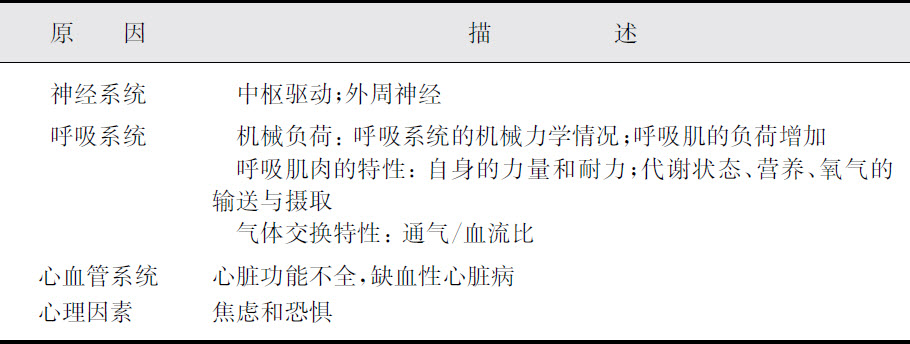
\includegraphics[width=\textwidth,height=\textheight,keepaspectratio]{./images/Image00303.jpg}
\end{longtable}

①神经系统因素:位于脑干的呼吸中枢功能失常,可以是结构上的(如脑干中风或中枢性窒息),也可以是代谢方面的(如电解质紊乱或镇静麻醉状态);代谢性或药物性因素也可导致外周神经功能失常。

②呼吸系统因素:呼吸肌方面包括废用性肌萎缩,严重的神经性肌病或药物(如神经肌肉阻滞剂、氨基糖甙类药物等)导致的肌病等;呼吸负荷增加常见于机体对通气的需求增加和呼吸力学的改变,如严重感染时通气需求增加,肺水肿、炎症、纤维化等导致肺的顺应性下降,支气管狭窄、炎症及狭窄的气管插管使气道阻力增加。

③代谢因素:营养、电解质和激素都是能够影响呼吸肌功能的代谢因素。营养不良导致蛋白质分解代谢和肌肉功能的减退;相反,摄食过度使CO\textsubscript{2}
产生过多,进一步增加了呼吸肌的通气负荷,故适当的营养支持能够增加撤机成功的概率。电解质缺乏也可损害呼吸肌功能,有研究表明血清磷水平正常可增加跨膈压。

④心血管因素:心功能储备较差的患者,降低通气支持可诱发心肌缺血或心力衰竭,其可能的机制包括:自主呼吸时代谢增加使循环的负荷增加;膈肌收缩使血液从腹腔转移至胸腔,导致回心血量增加;胸膜腔负压增加左心室后负荷。

⑤心理因素:恐惧和焦虑是导致撤机失败的非呼吸因素。

推荐意见10:对机械通气大于24小时不能撤机的患者,应尽快寻找原因。(B级)

\subsection{撤机筛查}

导致机械通气的病因好转或祛除后应开始进行撤机的筛查试验,筛查试验包括下列四项内容:

①导致机械通气的病因好转或祛除;

②氧合指标:PaO\textsubscript{2} /FiO\textsubscript{2}
>150~200;PEEP≤5~8cmH\textsubscript{2} O;FiO\textsubscript{2}
≤0.4~0.5;pH值≥7.25;COPD患者:pH值>7.30,PaO\textsubscript{2}
>50mmHg,FiO\textsubscript{2} <0.35;

③血流动力学稳定,没有心肌缺血动态变化,临床上没有显著的低血压(不需要血管活性药的治疗或只需要小剂量的血管活性药物如多巴胺或多巴酚丁胺<5~10μg/kg/分);

④有自主呼吸的能力。

\begin{longtable}{c}
  \caption{撤机常用的筛查标准}
  \label{tabapp-6}
  \endfirsthead
  \caption[]{撤机常用的筛查标准}
  \endhead
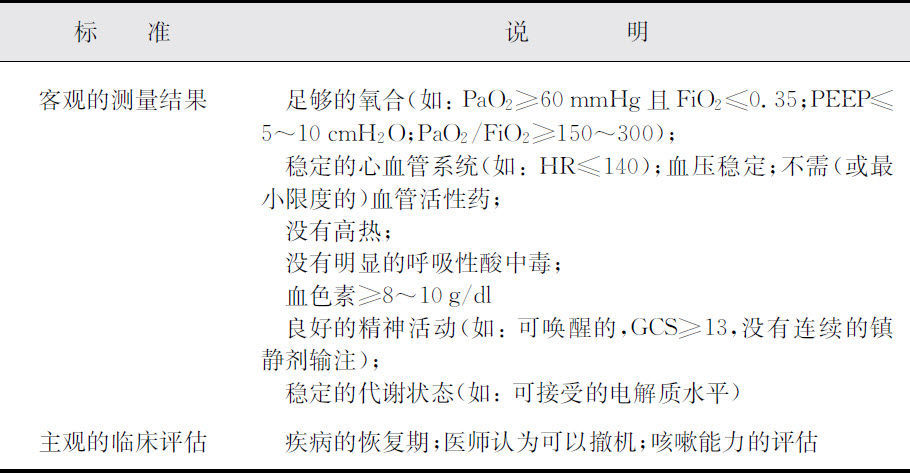
\includegraphics[width=\textwidth,height=\textheight,keepaspectratio]{./images/Image00304.jpg}
\end{longtable}

医师的经验影响撤机的过程及结果,临床常发生过早撤机或延迟撤机,增加再插管率。可接受的再插管率应该在5%~15%之间。再插管使患者的院内获得性肺炎增加8倍,死亡风险增加6~12倍。而不必要延长机械通气可增加患者感染和其他并发症的风险。不同的ICU患者中再插管率的变化范围是4%~23%,在精神和神经系统的患者中可高达33%。

推荐意见11:实施机械通气的原因被袪除后应开始进行撤机筛查试验(A级)

\subsection{自主呼吸试验}

符合筛查标准的患者并不一定能够成功的撤机,因此,需要对患者自主呼吸的能力作出进一步的判断,目前较准确的预测撤机的方法是三分钟自主呼吸试验,包括三分钟T管试验和CPAP5cmH\textsubscript{2}
O/psv试验,三分钟自主呼吸试验期间医生应在患者床旁密切观察患者的生命体征,当患者情况超出下列指标时应中止自主呼吸试验,转为机械通气:

①呼吸频率/潮气量(L)(浅快指数)应<105;

②呼吸频率应>8或<35次/分;

③自主呼吸潮气量应>4ml/kg;

④心率应<140次/分或变化<20%,没有新发的心律失常;

⑤氧饱和度应>90%。

三分钟自主呼吸通过后,继续自主呼吸30~120分钟,如患者能够耐受可以预测撤机成功,准备拔除气管插管。文献报道观察30分钟与120分钟的拔管成功率无差异,在SBT阶段进行监测评估,可以得到最有用的撤机信息以帮助临床决策。研究发现通过SBT30~120分钟的患者至少有77%可以成功撤机。导致SBT失败的原因有多种,但应注意气管插管引起的不适或持续气道内正压通气(CPAP)伺服阀不敏感/触发不良这些医源性因素。
 
\begin{longtable}{c}
  \caption{常用的耐受SBT的标准\textsuperscript{*}}
  \label{tabapp-7}
  \endfirsthead
  \caption[]{常用的耐受SBT的标准\textsuperscript{*}}
  \endhead
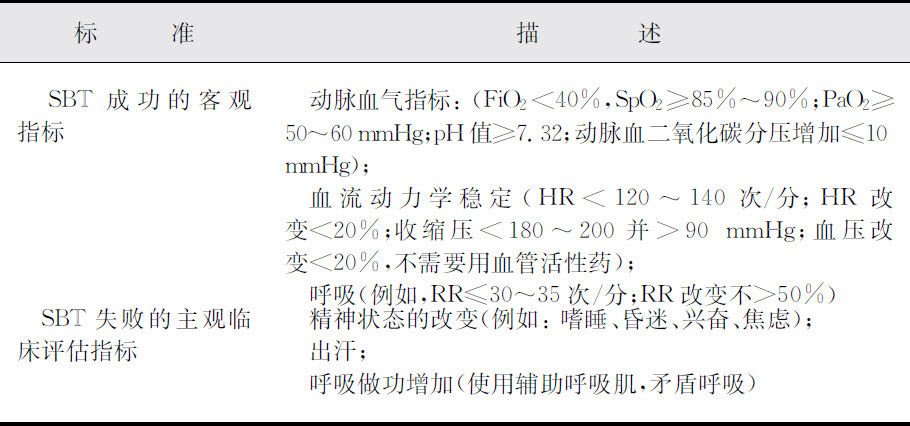
\includegraphics[width=\textwidth,height=\textheight,keepaspectratio]{./images/Image00305.jpg}\\
\footnotesize * HR=心率;SpO\textsubscript{2} =脉搏氧饱和度。
\end{longtable}




推荐意见12:通过筛查试验的患者,应进行自主呼吸试验(SBT)。(A级)

\subsection{气道评估}

拔管失败的原因与撤机失败的原因不同。上气道梗阻或患者气道保护能力差、气道分泌物清除能力不足。气管拔管后上气道梗阻的风险增加与机械通气的时间、女性、创伤和反复或创伤性插管有关。

气道通畅程度的评价;机械通气时,把气管插管的气囊放气以检查有无气体泄漏,可以用来评估上气道的开放程度(气囊漏气试验)。出现拔管后喘鸣的患者,可以使用类固醇和(或)肾上腺素[也可用无创通气和(或)氦氧混合气]治疗,而不需重新插管。如果患者漏气量较低,也可在拔管前24小时使用类固醇和(或)肾上腺素预防拔管后喘鸣。还应注意,漏气量变低可能是由于分泌物在气管插管周围结痂形成外皮所致而非上气道水肿狭窄。当漏气量低的患者拔管时,应将再插管的设备(包括气管切开设备)准备好。

气道保护能力的评价;患者的气道保护能力对拔管成功是至关重要的。对患者的气道评估包括吸痰时咳嗽的力度、有无过多的分泌物和需要吸痰的频率(吸痰频率应>2小时/次或更长)。在神经肌肉病变和脊髓损伤的患者中,有较好的咳嗽能力,预示可以拔管。

推荐意见13:对通过SBT的患者应评估气道通畅程度和保护能力。(B级)

\subsection{寻找SBT失败的原因}

SBT的失败后应立即寻找原因。常见的原因有镇痛镇静剂的使用不足、血容量不足、支气管痉挛和心肌缺血。

当SBT失败的原因纠正后每日进行一次SBT试验,没有必要一天内多次反复的进行SBT。呼吸系统异常很少在数小时内恢复,因此1天内频繁的SBT对患者没有帮助。Tobin的研究表明:SBT的失败的原因常是呼吸系统机械力学的异常,而这些异常不大可能迅速恢复。Esteban的试验证明,每天两次的SBT并不比每天一次更有优势。

SBT失败后,机械通气应选择恒定的支持水平,保证患者的呼吸肌充分休息,可以大大缩短训练的时间。所以在SBT失败后的24小时,应该让肌肉休息、舒适(包括使用镇静剂)和避免并发症,而不是积极的降低通气支持的水平。

一些通气模式[容量支持、适宜性辅助通气(ASV)、最小分钟通气量(MMV)],通过一个或多个呼吸周期测量参数的反馈,自动进行呼吸机撤离的评估。上述方法均可以安全地、自动地降低通气支持的水平。然而,这些模式中没有与每日SBT比较过。要证明这些自动化撤机方法的作用,还需要做更多工作。

近年来,ICU使用无创正压通气(NPPV)的应用日益增多。NPPV可以避免气管插管,也可帮助有创通气的撤离。两个慢性呼吸系疾病的前瞻性的随机对照试验的结果建议,拔管后给予NPPV辅助可以减少机械通气的时间、ICU的住院天数、病死率和医院获得性肺炎的发生率。

推荐意见14:若SBT失败,应给予充分的通气支持以缓解呼吸肌疲劳,并查找原因。(A级)

\subsection{术后机械通气患者的呼吸机撤离}

术后患者呼吸机的撤离是一个重要问题。术后患者24小时不能脱离呼吸机的主要原因是呼吸驱动力受到抑制和疼痛问题。适当的镇静、镇痛治疗方案有可能缩短机械通气的时间。

心脏术后患者5个随机对照试验证明,使用较低剂量的镇痛剂和镇静药物可提前拔管。

手术后患者的呼吸驱动力不够时,可应用辅助控制通气模式。对那些短时间恢复自主呼吸的患者,可降低通气支持水平,尽快撤机。

推荐意见15:术后机械通气患者应使用镇痛、镇静治疗方案(推荐级别A级)

\subsection{长期机械通气的撤机}

除非有明确的不可逆疾病的证据(例如,高位脊髓损伤或晚期的肌萎缩性脊髓侧索硬化),撤机失败3个月,为长期机械通气(permanent
mechanical ventilation,PMV)。

在20世纪80年代以前,这些患者长期在ICU中治疗,消耗了大量资源。对于康复的长期机械通气患者ICU不是适宜的治疗场所,应在医院内或医院外建立专门的撤机康复病房。部分长期机械通气的患者通过有计划的锻炼仍有撤机的希望,不能撤机的患者应制定终身的机械通气方案。

长期机械通气的患者很少采用每日自主呼吸试验,常使用辅助通气模式并逐步降低呼吸机条件以锻炼患者的呼吸肌。通常大约在通气支持条件降低到一半时,患者可转换到SBT步骤。撤机锻炼的过程中医务人员应留在患者身边,给予心理支持并小心避免不必要的肌肉疲劳。

推荐意见16:长期机械通气患者应采用逐步降低机械通气水平和逐步延长自主呼吸时间的撤机策略。(B级)

\textbf{中华医学会重症分会}

《机械通气临床应用指南(2006)》工作组

组长:秦英智(天津第三中心医院)

组员(按姓氏笔画):马晓春(中国医科大学附属第一医院)、王辰(首都医科大学朝阳医院)、方强(浙江大学医学院附属第一医院)、刘大为(中国医学科学院协和医院)、邱海波(东南大学附属中大医院)、席修明(首都医科大学附属北京复兴医院)、黎毅敏(广州呼吸病研究所)

\protect\hypertarget{text00036.html}{}{}

\chapter{2012重症成人患者疼痛、烦躁和谵妄处理临床实践指南}

2012年2月在休斯顿召开的美国危重症医学会(SCCM)年会上,镇静镇痛专家小组首次就历时6年完成的“重症成人患者疼痛、烦躁和谵妄处理临床实践指南”(Clinical
Practice Guidelinesforthe Management of Pain,Agitation,and Delirium in
Adult Patients in the Intensive Care
Unit,iPAD)进行了专题演讲,并阐述了相关建议。

\section{证据质量和建议力度}

证据质量:高(A)、中(B)、低/极低(C)。

建议力度:强烈(1),微弱(2),无建议(0)

\section{指 南}

\subsection{重症患者的疼痛、烦躁和谵妄的监测方法}

对比2002年指南,2012年指南专家组更强调了对疼痛、烦躁和谵妄的监测。在比较了6项疼痛尺度、10项镇静尺度和5项谵妄监测尺度后,筛选出了最适宜于重症患者疼痛、烦躁和谵妄的监测方法。

\subsubsection{疼痛的监测方法}

建议对所有重症成人患者常规进行疼痛监测(1B)。但疼痛是一种主观感觉,轻重程度难以用客观指标评估,因此不提倡单独用生命体征(或含生命体征的观察性疼痛尺度)进行重症医学科的疼痛评估(2C),但生命体征可作为需要进一步疼痛评估的依据(2C)。

对于神志清楚、可自我报告疼痛的患者,最可靠和有效的疼痛监测指标是患者的自述,可采用语言分层评分(verbal
rating scales)、视觉模拟评分(visual analogue
scales)或者面部表情评分法(faces pain
scale)进行监测;不能自我报告疼痛的患者(脑外伤除外),最有效和可靠的方法是疼痛行为量表(behavioral
pain
scale)(表\ref{tabapp-8})\footnote{* 总分3~12分,3分无痛,分值越高疼痛越重,12分最痛}和重症监护疼痛观察工具(critical-care-painobservation
tool)(B)(表\ref{tabapp-9})。

\begin{longtable}{c}
  \caption{疼痛行为量表\textsuperscript{*}}
  \label{tabapp-8}
  \endfirsthead
  \caption[]{疼痛行为量表\textsuperscript{*}}
  \endhead
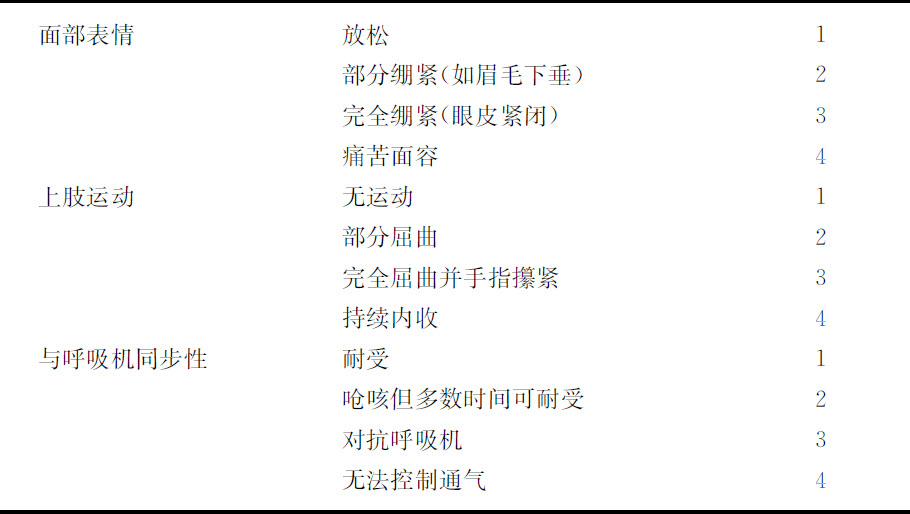
\includegraphics[width=\textwidth,height=\textheight,keepaspectratio]{./images/Image00306.jpg}
\end{longtable}


\begin{longtable}{c}
  \caption{重症监护疼痛观察工具}
  \label{tabapp-9}
  \endfirsthead
  \caption[]{重症监护疼痛观察工具}
  \endhead
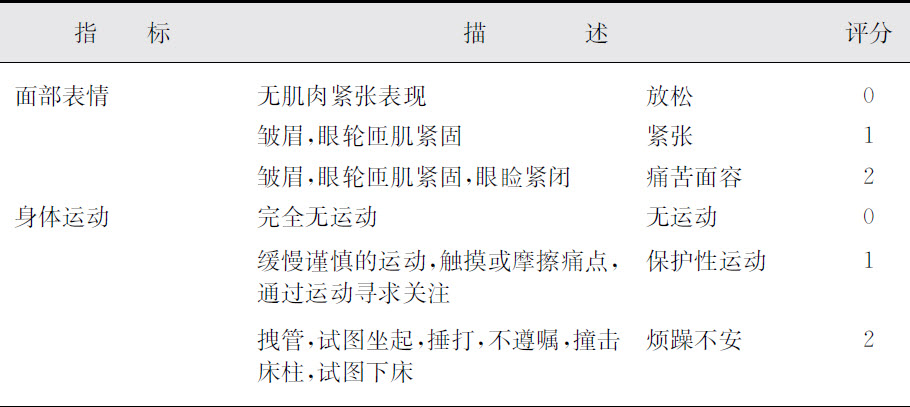
\includegraphics[width=\textwidth,height=\textheight,keepaspectratio]{./images/Image00307.jpg}\\
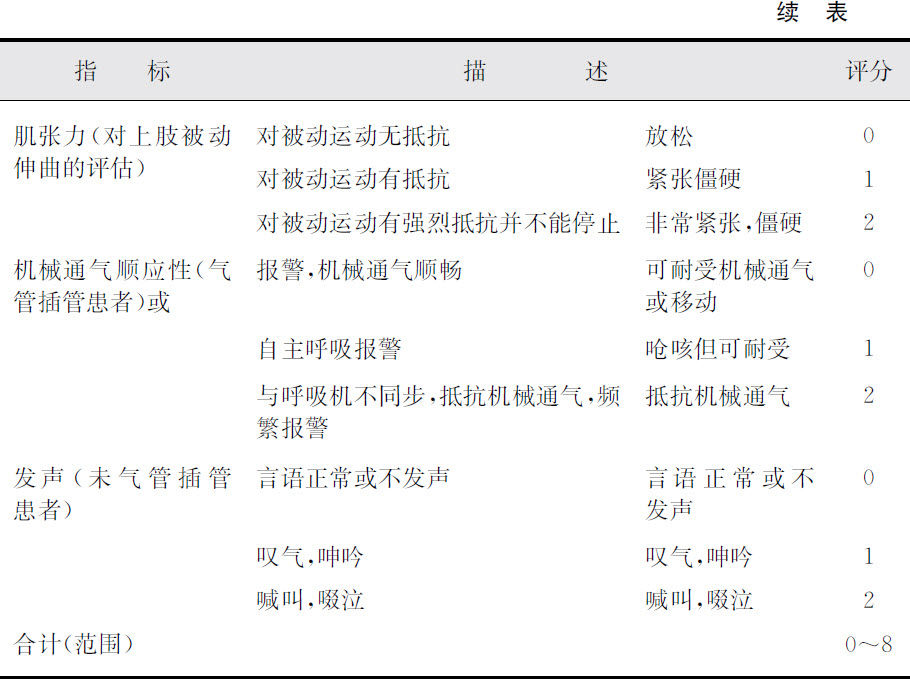
\includegraphics[width=\textwidth,height=\textheight,keepaspectratio]{./images/Image00308.jpg}
\end{longtable}

\subsubsection{躁动/镇静的监测方法}

对于非昏迷和非瘫痪的成人重症患者,不建议将脑功能客观监测作为镇静深度的主要监测手段。因其不足以替代主观性镇静评分系统(1B)。评估成人重症患者镇静质量和深度最可靠和有效的方法是Richmond躁动镇静评分(richmond
agitation-sedation scale)和镇静躁动评分(sedation-agitation
scale)(B),见表\ref{tabapp-10}、表\ref{tabapp-11}。

\begin{longtable}{c}
  \caption{Richmond躁动镇静评分}
  \label{tabapp-10}
  \endfirsthead
  \caption[]{Richmond躁动镇静评分}
  \endhead
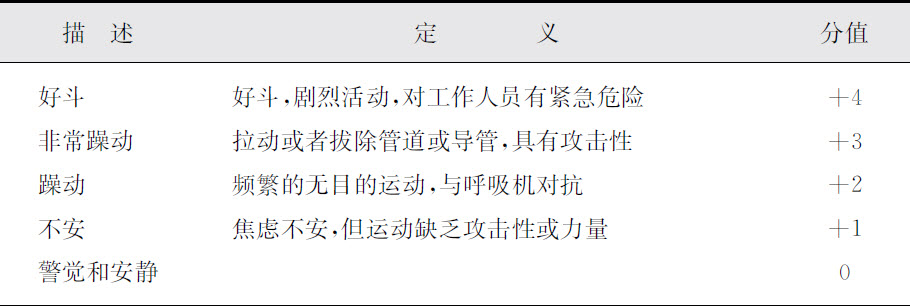
\includegraphics[width=\textwidth,height=\textheight,keepaspectratio]{./images/Image00309.jpg}\\
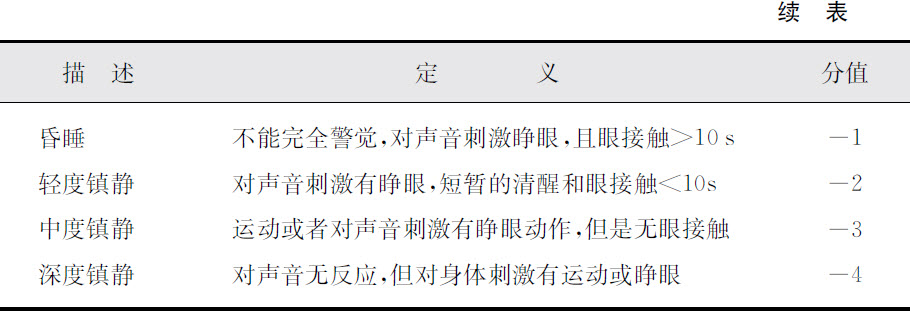
\includegraphics[width=\textwidth,height=\textheight,keepaspectratio]{./images/Image00310.jpg}
\end{longtable}

\begin{longtable}{c}
  \caption{镇静躁动评分}
  \label{tabapp-11}
  \endfirsthead
  \caption[]{镇静躁动评分}
  \endhead
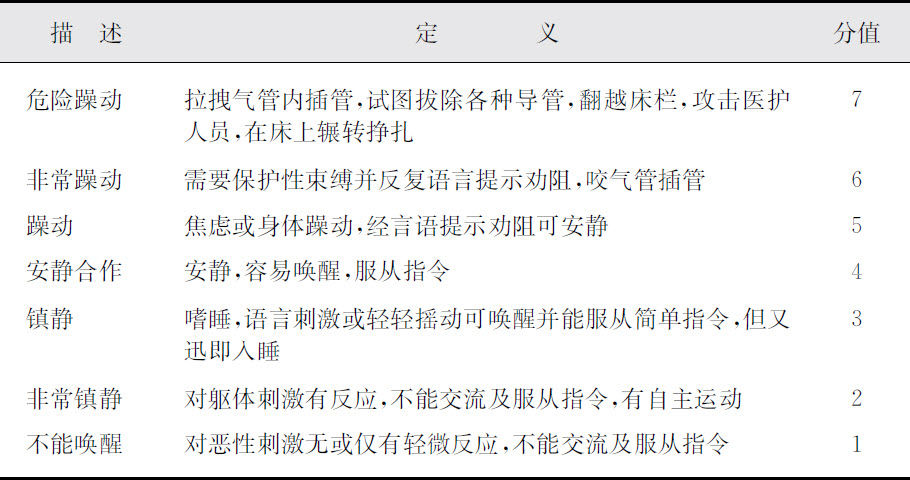
\includegraphics[width=\textwidth,height=\textheight,keepaspectratio]{./images/Image00311.jpg}
\end{longtable}

\subsubsection{谵妄的监测方法}

谵妄是由多种原因所致一过性的意识混乱状态,在重症发病率高达80%,患者一旦发生瞻望妄,将导致住院期延长、医疗费用及死亡率显著增加。因此建议对重症成人患者常规进行谵妄监测(1B)。最可靠和有效的重症成人患者谵妄监测手段是重症患者精神错乱评估法和重症谵妄评估量表。

重症患者精神错乱评估法主要包含以下几方面:①突然发作的精神状态改变或波动;②注意力不集中;③思维紊乱或意识清晰度下降。如果患者同时存在以上三个表现,则可诊断存在谵妄。

重症医学科谵妄评估量表见表\ref{tabapp-12}。\footnote{* 正常0分;1~3分=亚综合征谵妄(Subsyndromal Delirium);≥4分=谵妄}

\begin{longtable}{c}
  \caption{重症谵妄评估量表\textsuperscript{*}}
  \label{tabapp-12}
  \endfirsthead
  \caption[]{重症谵妄评估量表\textsuperscript{*}}
  \endhead
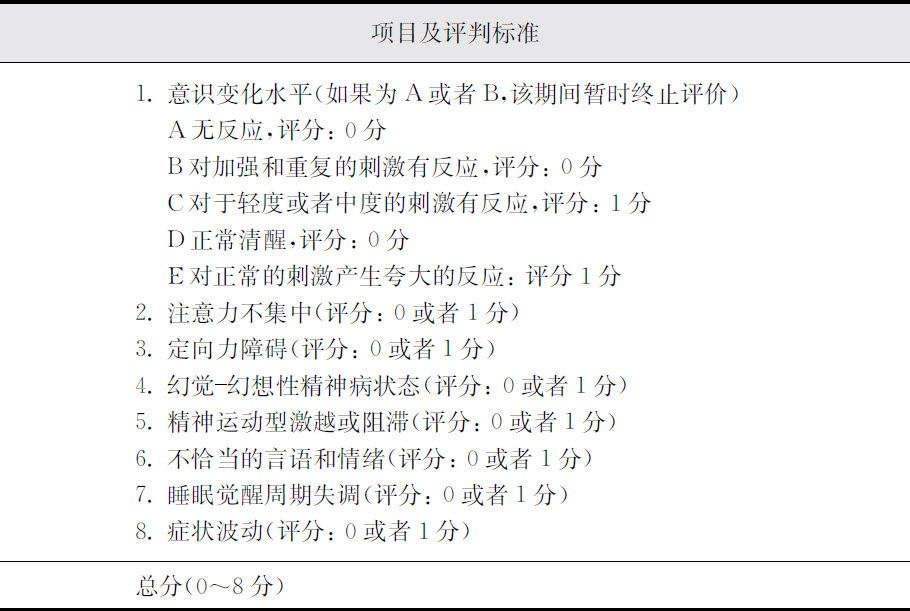
\includegraphics[width=\textwidth,height=\textheight,keepaspectratio]{./images/Image00312.jpg}
\end{longtable}

\subsection{重症成人患者疼痛、烦躁和谵妄的集束化治疗}

在SCCM2012年会上,“iPAD”指南小组制定了重症成人患者疼痛、烦躁和谵妄的集束化治疗,使重症成人患者镇静镇痛治疗更加规范化。

\subsubsection{疼痛的集束化治疗}

(1)疼痛评估:可自我报告患者采用视觉模拟评分、语言分层评分或面部表情评分进行评估;不能自我报告者采用疼痛行为量表或重症监护疼痛观察工具评估。

(2)疼痛治疗:

1)药物治疗:首选阿片类药物,可快速起效和消除疼痛。对非神经病性疼痛,静脉使用阿片类药物;对神经病性疼痛,静脉用阿片类药物加用肠内加巴喷丁或卡巴咪唑;应用非阿片类药物(醋氨酚、非甾体类消炎药、氯胺酮)有可能减少阿片类药物的剂量,并减少药物相关副作用。

2)非药物治疗:生物反馈、音乐治疗、放松等。

3)操作前预镇痛:提倡在重症医学科进行有创性和潜在疼痛性操作(比如拔除胸管)时采用预镇痛治疗,治疗方法是阿片类药物结合非药物治疗。

\subsubsection{烦躁的集束化治疗}

(1)评估镇静水平及相应处理:

1)每1~2小时评估Richmond躁动镇静评分或镇静躁动评分是否达标,如患者遵从指令、无烦躁或焦虑,则Richmond躁动镇静评分=0~-1、镇静躁动评分=4。

2)达到以上条件的患者,无需镇静;

3)镇静不足(Richmond躁动镇静评分>0、镇静躁动评分>4),给予镇静治疗;

4)镇静过度(Richmond躁动镇静评分<-1、镇静躁动评分<4),停用镇静镇痛治疗,评估至达到以上标准;重新开始镇静,起始用药剂量为先前剂量的50%。

(2)镇静治疗:

1)重症患者应在镇痛基础上进行镇静治疗,称为“镇痛性镇静”(analgosedation)或“镇痛为先的镇静”(analgesia-first
sedation,A-1sedation),可达到更为良好的镇静效果,并减少镇静药物用量。

2)建议对重症的成人患者调整镇静药物,维持浅水平镇静,而不是深度镇静,除非有临床禁忌(1B)。

3)建议对机械通气成人患者,常规采用每日中断镇静或靶水平浅镇静(1B)。

4)提倡首选非苯二氮䓬
镇静药(丙泊酚或右旋美托嘧啶),次选苯二氮䓬
药物(咪达唑仑或劳拉西泮),以便改善重症成人机械通气患者的临床结局(2B)。

\subsubsection{谵妄的集束化治疗}

(1)谵妄预防:预防策略包括控制疼痛、环境适应、优化睡眠觉醒周期、尽早开始活动、基础抗精神病药物治疗等。不提倡应用氟哌丁醇或非典型抗精神病药预防重症成人患者谵妄。

(2)谵妄评估:入住重症患者应在每6~12小时进行谵妄评估,采用重症患者精神错乱评估法或重症医学科谵妄评估量表评分进行评估。

(3)谵妄治疗:对于存在谵妄(重症患者精神错乱评估法阳性或重症医学科谵妄评估量表评分≥4)的患者,应积极治疗谵妄。

1)药物治疗:①有待发表的研究证据显示应用氟哌丁醇治疗谵妄可缩短重症成人患者的谵妄持续时间。②非典型抗精神病药可能缩短重症成人患者的谵妄持续时间(奥氮平、氯氮平)。③不建议使用非典型抗精神病药用于有尖端扭转室速风险患者的谵妄治疗。这类患者主要包括基础QT间期延长患者、合并使用已知可延长QT间隙药物的患者、曾经发生尖端扭转室速)。④对于与酒精或苯二氮䓬
类药物撤除无关的重症成人患者的谵妄,建议应用右旋美托咪啶而并非苯二氮䓬
类药物治疗。

2)非药物治疗:

避免使用诱导谵妄的药物。

建议对重症成人患者一旦有可能即早期活动以便减少谵妄的发生。

\protect\hypertarget{text00037.html}{}{}

\chapter{2012成人严重感染和感染性休克治疗指南}

严重感染和感染性休克临床患病率高,治疗困难,显著影响重症患者预后。各国重症医学领域和感染性疾病专家组成委员会(surviving
sepsis
campaign,SSC)就严重感染和感染性休克的诊治达成共识,制定了严重全身性感染和感染性休克的治疗指南,该指南于2004年首次发布,2008年更新后,于2012年再次更新,以进一步提高对严重感染和感染性休克的认识并改善患者预后。指南制定的治疗措施的推荐级别和分级标准见\ref{tabapp-13}。


\begin{longtable}{c}
  \caption{治疗措施的推荐级别和分级标准}
  \label{tabapp-13}
  \endfirsthead
  \caption[]{治疗措施的推荐级别和分级标准}
  \endhead
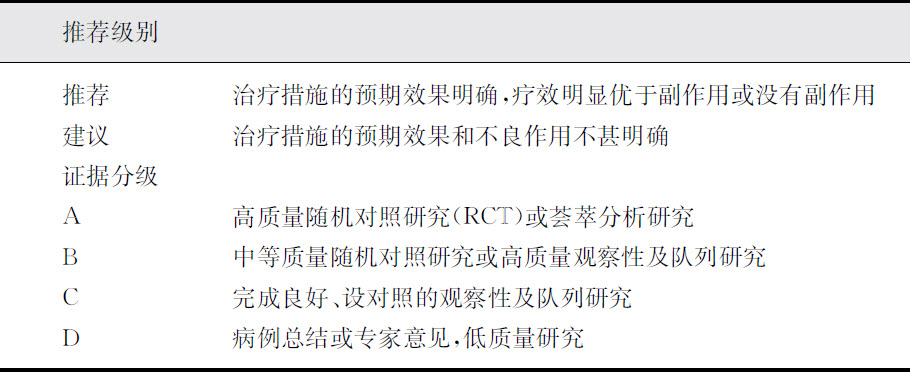
\includegraphics[width=\textwidth,height=\textheight,keepaspectratio]{./images/Image00317.jpg}
\end{longtable}


A.早期液体复苏

1.推荐对于存在组织低灌注(经初步液体复苏仍存在低血压或血乳酸>4mmol/L)的感染性休克患者尽早进行液体复苏。复苏最初6小时目标:中心静脉压(CVP)8~12mmHg,平均动脉压(MAP)≥65mmHg,尿量≥每小时0.5ml/kg,中心静脉血氧饱和度(SvO\textsubscript{2}
)≥70%或混合动静脉血氧饱和度(ScvO\textsubscript{2} )≥65%(1C)。

2.建议对于以乳酸增高为表现的组织低灌注患者,尽快给予液体复苏将乳酸降至正常水平(2C)。

B.感染的筛查

推荐对所有重症患者进行早期感染的评价,尽早明确有无感染存在,对可疑感染患者留取标本进行病原学检查以指导目标性抗感染治疗(1C)。

C.感染的诊断

1.推荐只要留取标本进行培养的时间不超过45分钟,都应在使用抗生素前留取标本进行病原微生物的培养(1C)。为最有效地获得病原学证据,建议抗生素使用之前至少要留取两份血培养,一份经皮穿刺血标本,一份为导管留置时间大于48小时的导管血标本;同时,应尽可能在使用抗生素之前留取其他可疑感染部位的标本进行培养,包括尿液、脑脊液、伤口、呼吸道分泌物或可能为感染源的其他体液(1C)。

2.对于早期侵袭性念珠菌感染的诊断,建议进行血清1,3β-D-葡聚糖检测(2B)、血清甘露聚糖和抗甘露聚糖抗体检测(2C)

3.推荐尽快行影像学检查以明确有无潜在的感染病灶(UG)。

D.抗感染治疗

1.推荐确认感染性休克1小时内(1B)或严重感染但尚未出现感染性休克(1C)时尽早静脉使用抗生素治疗。在应用抗生素之前留取合适的标本,但不能为留取标本而延误抗生素的使用。

2a.由于严重感染和感染性休克患者病死率高,推荐最初的经验性抗感染治疗包括可覆盖所有可疑病原微生物[细菌和(或)真菌或病毒]的一种或多种药物,并且要求药物对感染病灶有足够高的穿透能力,以保证感染病灶中足够高的药物浓度(1B)。

2b.推荐每天评价抗生素治疗方案的疗效,以达到理想的临床治疗效果,防止细菌耐药产生,减少药物毒性并降低治疗费用(1B)

3.建议低水平降钙素原等生物标记物有助于临床医师停止没有后续感染患者的经验性抗生素使用(2C)。

4a.建议对中性粒细胞减少症患者进行经验性联合治疗(2B)。对已知或怀疑为难治性、多药耐药的细菌如不动杆菌和假单胞菌属等引起的感染,进行经验性的联合治疗(2B)。对于合并呼吸衰竭和感染性休克的严重绿脓杆菌感染患者,选择联合广谱β内酰胺、氨基糖苷类或喹诺酮类药物治疗(2B)。对于肺炎链球菌感染的感染性休克患者,选择联合广谱β内酰胺和大环内酯类药物治疗(2B)。

4b.经验性抗生素治疗时,建议联合治疗不超过3~5天。一旦致病菌明确,应选择最恰当的单一治疗(2B)。

5.建议抗感染疗程一般为7~10天,但对于临床治疗反应慢、感染病灶没有完全清除、金黄色葡萄球菌病毒或真菌感染或免疫缺陷(包括中性粒细胞减少症)患者,可适当延长疗程(2C)

6.建议对于由病毒感染,如流感病毒导致的感染性休克患者,应尽早采取抗病毒治疗,并及时寻找病毒感染的证据(2C)。

7.推荐对于明确由非感染因素导致严重炎症反应状态的患者应立即停止抗生素治疗,以减少继发耐药菌感染或出现药物相关副作用(UG)

E.感染源的控制

1.推荐对一些需紧急处理的感染如坏死性筋膜炎、弥漫性腹膜炎、胆管炎、肠坏死等要尽快明确诊断,并在明确诊断后12小时进行外科引流以控制感染来源(1C)。

2.建议对确定为胰腺周围坏死并可能成为潜在感染灶者,最好待有活力组织和坏死组织界限明确划分之后,再进行干预(2B)

3.在需要进行感染源治疗时,推荐采用对生理损伤最小的有效干预措施(例如对脓肿进行经皮引流而不是外科引流)(UG)。

4.建立血管通路后,应立即去除那些可能成为严重感染或感染性休克感染灶的血管内装置(UG)。

F.感染预防

1a.建议通过选择性口腔去污染(SOD)和选择性消化道去污染(SDD)减少呼吸机相关性肺炎(VAP)发生(2B),该措施也适用于健康护理机构的患者。

1b.建议应用洗必泰进行口腔护理,以减少严重感染的重症患者VAP的发生(2B)。

G.严重感染的液体治疗

1.推荐对严重感染和感染性休克患者应用晶体液进行初始液体复苏(1B)。

2.建议对需大剂量晶体液复苏的严重感染和感染性休克患者加用白蛋白进行初始液体复苏(2C)。

3.不建议使用羟乙基淀粉进行液体复苏(1B)。

4.推荐对怀疑有低血容量状态的感染患者进行液体复苏时,液体复苏的量至少为30ml/kg的晶体液(可能包含部分等量的胶体),有些患者可能需要更多的复苏液体量、更快的复苏速度(1C)。

5.推荐对采用液体负荷试验、利用动态或静态指标判断容量反应性显示血流动力学可得到改善的患者,可继续行液体治疗(UG)。

H.血管活性药物

1.推荐使用血管加压药物维持MAP保持≥65mmHg(1C)。

2.推荐去甲肾上腺素为首选升压药物(1B)。

3.需要附加药物维持目标血压时,推荐去甲肾上腺素的基础上加用肾上腺素,或肾上腺素取代去甲肾上腺素(2B)。

4.建议使用血管加压素0.03U/分联合或取代去甲肾上腺素维持血压(UG)。

5.不推荐低剂量的血管加压素作为重症感染低灌注的单一初始血管活性药,血管加压素剂量>0.03~0.04U/分作为抢救治疗时应保留。

6.建议对于经严格选择的特殊患者(不易出现心律失常、明确的显著的左心收缩功能障碍或心率减慢患者)使用多巴胺作为去甲肾上腺素的替代治疗(2C)。

7.不推荐去氧肾上腺素作为感染性休克的治疗,除非使用去甲肾上腺素时出现严重心律失常,或心排血量高但血压持续降低,或其他药物升压无效(1C)。

8.推荐不使用小剂量多巴胺用于肾脏保护(1A)。

9.推荐所有使用血管活性药物的患者尽可能放置动脉导管监测血压(UG)。

I.正性肌力药物治疗

1.推荐对存在心脏充盈压升高、心输出量降低提示心肌功能障碍的患者、或持续低灌注的患者,应用或在血管加压药治疗的基础上静脉滴注多巴酚丁胺增强心肌收缩力,多巴酚丁胺最大剂量每分钟20μg/kg(1C)。

2.推荐不使用将心指数提高到超常水平的治疗策略(1B)。

J.糖皮质激素治疗

1.对液体复苏和血管加压药治疗不敏感的成人感染性休克患者,推荐静脉氢化可的松治疗(2C),每天用量不超过200mg。

2.不建议通过ACTH兴奋试验鉴别须接受糖皮质激素治疗的成人感染性休克患者(2B)。

3.当患者不再需要血管升压药维持循环时,建议停用糖皮质激素治疗(2D)。

4.没有感染性休克的患者,不推荐使用糖皮质激素(1D)。

5.应用小剂量氢化可的松时,建议连续静脉使用而不是重复冲击使用(2D)。

K.血制品应用

1.一旦患者组织低灌注得以改善、没有心肌缺血、重度低氧血症、急性失血、心脏疾病等,推荐只有当血红蛋白低于70g/L、而不是低于90g/L时输注红细胞,使血红蛋白维持在70~90g/L(1B)。

2.不推荐使用促红细胞生成素治疗感染相关的贫血(1B)。

3.当没有活动性出血或不计划行侵袭性操作时,不建议输注新鲜冰冻血浆纠正凝血功能障碍(2D)。

4.不推荐严重感染和感染性休克患者使用抗凝血酶(1B)。

5.对于严重感染患者,建议当血小板计数<10×10\textsuperscript{9}
/L时,无论是否有出血,都应输注血小板。如果患者有明显出血倾向,当血小板计数<20×10\textsuperscript{9}
/L应输注血小板。当患者出现活动性出血或需进行外科手术或进行有创性操作时,应维持血小板计数≥50×10\textsuperscript{9}
/L(2D)。

L.免疫球蛋白的使用

不建议对严重感染和感染性休克的成年患者静脉输注免疫球蛋白(2B)。

M.硒

不建议静脉输注硒治疗严重感染(2C)。

N.rhAPC的使用

由于rhAPC不再推荐使用,新指南只提供历史推荐意见。

O.严重感染所致急性肺损伤(ALI)/急性呼吸窘迫综合征(ARDS)的机械通气治疗。

1.推荐对于严重感染所致ALI/ARDS患者设定6ml/kg而非12ml/kg理想体重的潮气量(1A)。

2.推荐监测ALI/ARDS患者平台压,初始平台压高限不超过30cmH\textsubscript{2}
O(1B)。

3.推荐设定PEEP以防止呼气末肺泡萎陷(1B)。

4.建议对于严重感染所致中度或重度ARDS患者实施高水平PEEP的通气策略而不是低水平PEEP的通气策略(2C)。

5.建议对于严重难治性低氧血症的严重感染患者实施肺复张(2C)。

6.建议在有经验的单位,对于严重感染所致的ARDS患者,当PaO\textsubscript{2}
/FiO\textsubscript{2} <100mmHg采取俯卧位通气(2B)。

7.机械通气的感染性休克患者如无禁忌证,推荐床头抬高30~45°,以防止误吸和VAP(1B)。

8.建议少数利大于弊的ALI/ARDS患者可以谨慎使用无创通气治疗(2B)。

9.推荐对符合以下条件的患者常规进行自主呼吸测试:清醒,血流动力学稳定(无血管活性药物使用),无新发潜在的严重疾病,低PEEP水平,通过面罩或鼻导管吸氧可获得的低吸氧浓度。满足上述条件则拔除气管插管(1A)。

10.反对常规使用肺动脉导管(1A)。

11.推荐对于没有组织低灌注的患者采用限制性液体管理策略(1C)。

12.对于不存在支气管痉挛的ARDS患者,不推荐使用β\textsubscript{2}
受体激动剂。

P.严重感染的镇静、麻醉、肌松

1.推荐对于机械通气患者间歇注射或连续点滴达到预定镇静目标(1B)。

2.鉴于停药后肌松药作用持续时间较长,推荐对无ARDS的感染性休克患者避免应用肌松药(NMBA)。如果必须应用,应间断推注,或在持续滴注过程中使用4连串刺激监测阻滞深度(1C)。

3.建议对于严重感染导致的ARDS患者病程早期、氧合指数(PaO\textsubscript{2}
/FiO\textsubscript{2}
)<150mmHg时,应用NMBA治疗,使用时间不应超过48小时(2C)。

Q.血糖控制

1.对于严重感染患者,如果连续两次检测血糖值>10mmol/L,推荐使用有效方案调整胰岛素剂量控制血糖水平,使最高血糖水平低于10mmol/L而不是低于6.1mmol/L(1A)。

2.推荐每1~2小时监测一次血糖,血糖和胰岛素用量稳定后,可每4小时监测一次(1C)。

3.推荐用床旁快速检测法监测末梢血糖水平时,如果血糖值较低,应予以重视,因为动脉血或血浆葡萄糖水平可能比检测的末梢血糖值更低(UG)。

R.肾脏替代治疗

1.对重症感染合并急性肾衰竭患者,连续肾脏替代治疗与间断血液透析等效(2B)。

2.对血流动力学不稳定者,建议采用持续肾替代治疗,以利于液体平衡的控制(2D)。

S.碳酸氢盐治疗

1.不推荐对低灌注致高乳酸血症、pH≥7.15的患者使用碳酸氢钠改善血流动力学或减少升压药使用(2B)。

T.预防深静脉血栓形成

1.对严重感染患者应进行DVT的药物预防,推荐每日皮下注射低分子量肝素(LMWH)、而不是使用小剂量普通肝素(UFH)预防深静脉血栓(DVT)(1B)。如果患者肌酐清除率<30ml/分,使用达肝素钠(1A),或使用其他类型的低肾代谢的低分子肝素(2C),或使用肝素(1A)。

2.如果不能使用LMWH,推荐使用UFH每日3次(1C)。

3.建议对严重感染的患者行药物治疗联合间断气体加压治疗预防深静脉血栓形成(2C)。

4.对于肝素使用有禁忌的患者(如血小板减少、严重凝血功能障碍、活动性出血、近期脑出血),不进行药物预防(1B),推荐使用器械预防措施如弹力袜或间断气体加压治疗预防深静脉血栓形成(2C)。当出血风险降低后开始使用药物预防(2C)。

U.应激性溃疡的预防

1.推荐对有出血危险因素的严重感染/感染性休克患者预防应用H2受体阻断剂或质子泵抑制剂(1B)。

2.预防应激性溃疡时,建议首选质子泵抑制剂而不是H2受体阻断剂(2D)。

3.建议无出血危险因素的患者不进行应激性溃疡的预防(2B)。

V.营养

1.建议对于诊断为严重感染/感染性休克的患者,初始48小时内尽可能实施口服或肠内营养(如有必要),而不是禁食或者仅给予葡萄糖输注(2C)。

2.初始48小时内避免强制给予全能量喂养,而建议给予小剂量喂养(例如最高每天500kcal),只有当患者能耐受时增加喂养量(2B)。

3.建议诊断严重感染/感染性休克7天内使用静脉输注葡萄糖和肠内营养相结合,而不是单独给予全肠外营养(TPN)或者肠外营养与肠内营养相结合的喂养(2B)。

4.对于严重感染的患者使用不加特定免疫增强剂的营养物而不是带有免疫增强剂的营养物(2C)。

W.设定治疗目标

1.推荐与患者家属沟通患者的治疗目标和预后(1B)。

2.推荐将治疗目标整合入治疗和临终关怀计划当中,并恰当应用安慰治疗原则(1B)。

3.建议尽早制定明确的治疗目标,最迟不超过入科后72小时(2C)。

\protect\hypertarget{text00038.html}{}{}

\chapter{KIDGO急性肾损伤诊疗指南}

急性肾损伤的发病率逐年升高。该指南根据2011年2月以前的文献资料制定和撰写。以指导急性肾损伤的临床诊断和治疗决策的制定。

该指南推荐意见的级别分为3级,即推荐、建议和未分级。推荐意见的支持证据质量分为4级,A~D级,其中A级最高,D级最低(表\ref{tabapp-14})。

\begin{longtable}{c}
  \caption{指南支持证据质量}
  \label{tabapp-14}
  \endfirsthead
  \caption[]{指南支持证据质量}
  \endhead
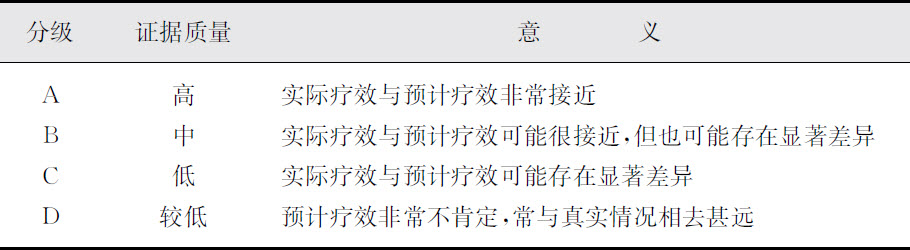
\includegraphics[width=\textwidth,height=\textheight,keepaspectratio]{./images/Image00318.jpg}
\end{longtable}

1.急性肾损伤(AKI)定义

1.1 急性肾损伤的定义与分级

1.1.1 急性肾损伤的定义为以下任何一项 未分级

·48小时内血肌酐增加≥0.3mg/dl(≥26.5μmol/L);或

·已知或推测过去7天内血肌酐增加至≥基础值的1.5倍;或

·尿量<每小时0.5ml/kg持续6小时

1.1.2 根据以下标准对急性肾损伤的严重程度进行分级(表\ref{tabapp-15}) 未分级

\begin{longtable}{c}
  \caption{急性肾损伤分级}
  \label{tabapp-15}
  \endfirsthead
  \caption[]{急性肾损伤分级}
  \endhead
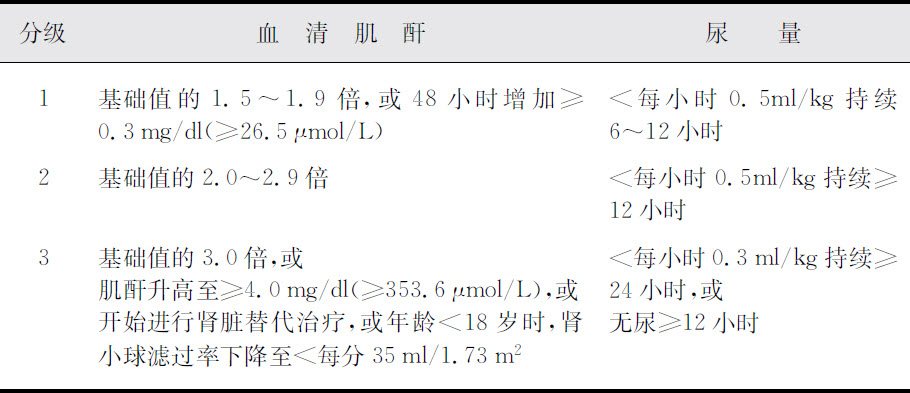
\includegraphics[width=\textwidth,height=\textheight,keepaspectratio]{./images/Image00319.jpg}
\end{longtable}

1.1.3 应当尽可能确定急性肾损伤的病因 未分级

1.2 风险评估

1.2.1 推荐根据患者的易感性和暴露情况对急性肾损伤风险进行分级 1B

1.2.2 根据患者的易感性和暴露情况进行治疗以减少发生急性肾损伤的风险 未分级

1.2.3 对急性肾损伤高危患者,测定血肌酐和尿量变化以早期诊断急性肾损伤 未分级

1.3 急性肾损伤高危患者的评估和一般治疗

1.3.1 及时对急性肾损伤患者进行评估,以确定病因,尤其应当注意可逆因素 未分级

1.3.2 通过测定血肌酐和尿量对急性肾损伤患者进行监测,\\
并依照1.1.2的推荐意见对急性肾损伤的严重程度进行分级 未分级

1.3.3 根据分级和病因对急性肾损伤患者进行治疗(表\ref{tabapp-16}) 未分级

\begin{longtable}{c}
  \caption{根据分级对急性肾损伤患者进行治疗急性肾损伤分级}
  \label{tabapp-16}
  \endfirsthead
  \caption[]{根据分级对急性肾损伤患者进行治疗急性肾损伤分级}
  \endhead
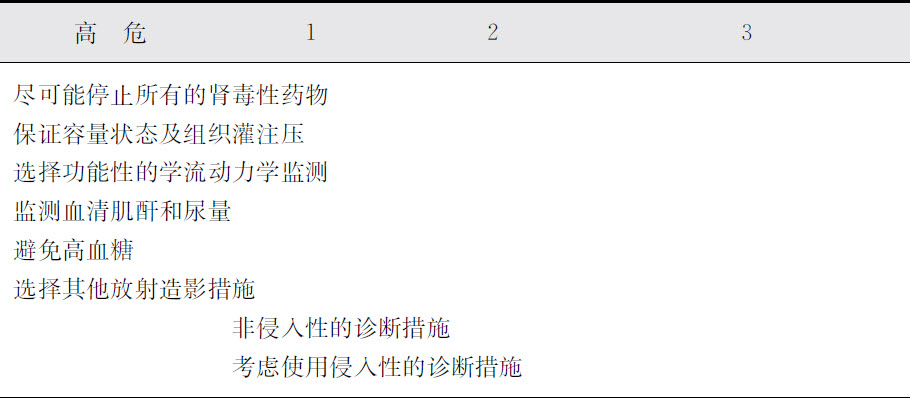
\includegraphics[width=\textwidth,height=\textheight,keepaspectratio]{./images/Image00320.jpg}\\
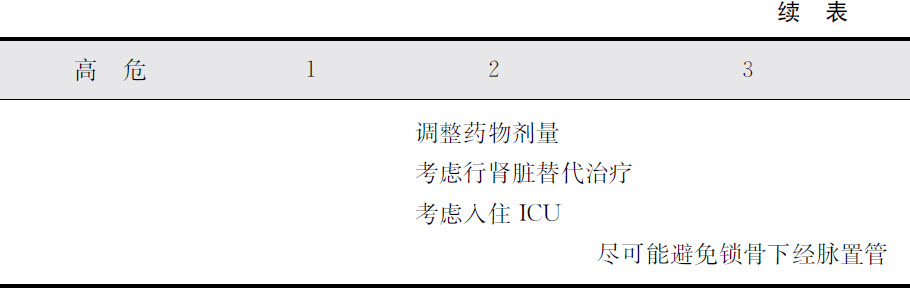
\includegraphics[width=\textwidth,height=\textheight,keepaspectratio]{./images/Image00321.jpg}
\end{longtable}

1.3.4 发生急性肾损伤后3个月对病情恢复、新发或既往慢性肾脏疾病加重情况进行评估 未分级

·如果患者发生慢性肾脏疾病,应当根据KDOQI慢性肾脏疾病指南进行治疗 未分级

·即使未发生慢性肾脏疾病,仍应将其作为慢性肾脏疾病的高危人群,并根据KDOQI慢性肾脏疾病指南中有关慢性肾脏疾病高危患者的推荐意见进行治疗 未分级

2.急性肾损伤的预防和治疗

2.1 血流动力学监测和支持治疗以预防和治疗急性肾损伤

2.1.1 在没有失血性休克的情况下,建议使用等张晶体液而非胶体液(白蛋白或淀粉)作为急性肾损伤高危患者或急性肾损伤患者扩容治疗的初始选择 2B

2.1.2 对于分布性休克合并急性肾损伤或急性肾损伤高危患者,推荐联合使用升压药物和液体复苏治疗 1C

2.1.3 对于围手术期高危患者或感染性休克患者,建议根据治疗方案纠正血流动力学和氧代谢紊乱,以防止急性肾损伤的发生或恶化 2C

2.2 血糖控制与营养支持

2.2.1 对于重症患者,建议使用胰岛素治疗维持血糖在110~149mg/dl(6.1~8.3mmol/L) 2C

2.2.2 对于任何阶段的急性肾损伤患者,建议总热量摄入应达到每天20~30kcal/kg 2C

2.2.3 建议不限制蛋白质摄入,以预防或延迟肾脏替代治疗的治疗 2D

2.2.4 对于无需透析治疗的非分解代谢急性肾损伤患者,建议补充蛋白质每天0.8~1.0g/kg 2D\\
对于使用肾脏替代治疗的急性肾损伤患者,蛋白质补充每天1.0~1.5g/kg\\
对于使用连续肾脏替代治疗或高分解代谢的患者,蛋白质补充应不超过每天1.7g/kg

2.2.5 建议急性肾损伤患者优先选择肠内营养支持 2C

2.3 利尿剂的使用

2.3.1 推荐不使用利尿剂预防急性肾损伤 1B

2.3.2 建议不使用利尿剂治疗急性肾损伤,除非在容量过负荷时 2C

2.4 血管扩张药物治疗:多巴胺,非诺多巴及利钠肽

2.4.1 建议不使用小剂量多巴胺预防或治疗急性肾损伤 1A

2.4.2 建议不使用非诺多巴(fenoldopam)预防或治疗急性肾损伤 2C

2.4.3 建议不使用心房利钠肽(ANP)预防(2C)或治疗(2B)急性肾损伤

2.5 生长激素治疗\\
推荐不使用重组人(rh)IGF 1预防或治疗急性肾损伤 1B

2.6 腺苷受体拮抗剂\\
对于围产期严重窒息的急性肾损伤高危新生儿,建议给予单一剂量的茶碱 2B

2.7 预防氨基糖甙和两性霉素相关急性肾损伤

2.7.1 建议不使用氨基糖甙类药物治疗感染,除非没有其他更为适合、肾毒性更小的治疗药物选择 2A

2.7.2 对于肾功能正常且处于稳定状态的患者,建议氨基糖甙类药物每日给药一次,而非每日多次给药 2B

2.7.3 当氨基糖甙类药物采用每日多次用药方案,且疗程超过24小时,推荐监测药物浓度 1A

2.7.4 当氨基糖甙类药物采用每日一次用药方案,且疗程超过48小时,建议监测药物浓度 2B

2.7.5 建议必要时局部使用(例如呼吸道雾化吸入,抗生素分子渗透)而非静脉应用氨基糖甙类药物 2B

2.7.6 建议使用脂质体两性霉素B而非普通两性霉素B 2A

2.7.7 治疗全身性真菌或寄生虫感染时,如果能达到相同疗效,推荐使用唑类抗真菌药物和(或)棘白菌素类药物,而非普通两性霉素B 1A

2.8 其他预防重症患者发生急性肾损伤的措施

2.8.1 建议不要单纯为减少围手术期急性肾损伤或肾脏替代治疗需求而采用不停跳冠状动脉搭桥术 2C

2.8.2 对于合并低血压的重症患者,建议不使用N-乙酰半胱氨酸预防急性肾损伤 2D

2.8.3 推荐不使用口服或静脉N-乙酰半胱氨酸预防术后急性肾损伤 1A

3.造影剂诱导急性肾损伤

3.1 造影剂诱导急性肾损伤:定义,流行病学和预后血管内使用造影剂后,应当根据推荐意见1.1.1---1.1.2对急性肾损伤进行定义和分级 未分级

3.1.1 对于血管内使用造影剂后肾脏功能改变的患者,应当对造影剂相关急性肾损伤及急性肾损伤的其他可能原因进行评估 未分级

3.2 造影剂相关急性肾损伤高危人群评估

3.2.1 对于需要血管内(静脉或动脉)使用碘造影剂的所有患者,应当评估发生造影剂相关急性肾损伤的风险,尤其应对既往肾脏功能异常者进行筛查 未分级

3.2.2 对于造影剂相关急性肾损伤高危患者,应当考虑其他造影方法 未分级

3.3 造影剂相关急性肾损伤的非药物干预措施

3.3.1 对于造影剂相关急性肾损伤高危患者,应当使用最小剂量的造影剂 未分级

3.3.2 对于造影剂相关急性肾损伤高危患者,推荐使用等渗或低渗碘造影剂,而非高渗碘造影剂 1B

3.4 造影剂相关急性肾损伤的药物预防措施

3.4.1 对于造影剂相关急性肾损伤高危患者,推荐静脉输注等张氯化钠或碳酸氢钠溶液进行液体补充 1A

3.4.2 对于造影剂相关急性肾损伤高危患者,推荐不单独使用口服补液 1C

3.4.3 对于造影剂相关急性肾损伤高危患者,建议口服N-乙酰半胱氨酸联合静脉等张晶体液 2C

3.4.4 建议不使用茶碱预防造影剂相关急性肾损伤 2C

3.4.5 推荐不使用非诺多巴预防造影剂相关急性肾损伤 2C

3.5 血液透析或血液滤过的作用

3.5.1 对于造影剂相关急性肾损伤高危患者,建议不预防性使用间断血液透析或血液滤过清除造影剂 2C

4.透析治疗急性肾损伤

4.1 急性肾损伤肾脏替代治疗的时机

4.1.1 出现危及生命的容量、电解质和酸碱平衡改变时,应紧急开始肾脏替代治疗 未分级

4.1.2 作出开始肾脏替代治疗的决策时,应当全面考虑临床情况,是否存在能够被肾脏替代治疗纠正的情况,以及实验室检查结果的变化趋势,而不应仅根据尿素氮和肌酐的水平 未分级

4.2 急性肾损伤停止肾脏替代治疗的标准

4.2.1 当不再需要肾脏替代治疗时(肾脏功能恢复至足以满足患者需求,或肾脏替代治疗不再符合治疗目标),应当终止肾脏替代治疗 未分级

4.2.2 建议不使用利尿剂促进肾脏功能恢复、缩短肾脏替代治疗疗程或降低肾脏替代治疗治疗频率 2B

4.3 抗凝

4.3.1 对于需要肾脏替代治疗的急性肾损伤患者,需评估患者从抗凝中获得的利与弊来决定是否抗凝(图\ref{figapp-1}) 未分级


\begin{figure}[!htbp]
    \centering
    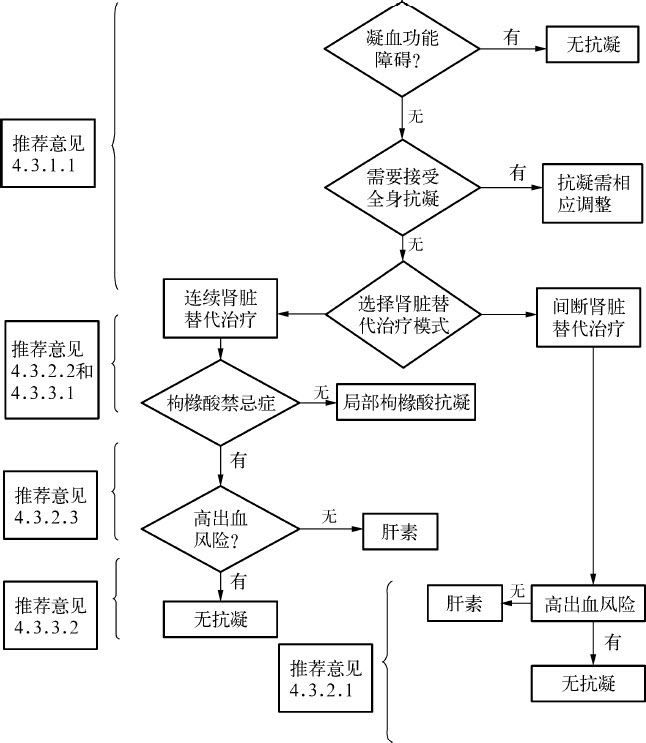
\includegraphics{./images/Image00322.jpg}
    \captionsetup{justification=centering}
    \caption{肾脏替代治疗治疗抗凝流程}
    \label{figapp-1}
\end{figure} 

4.3.1.1 如果急性肾损伤患者没有明显的出血风险或凝血功能障碍,且未接受全身抗凝治疗,推荐在肾脏替代治疗期间使用抗凝 1B

4.3.2 对于没有高危出血风险或凝血功能障碍、且未接受有效全身抗凝治疗的患者,有以下建议:

4.3.2.1 对于间断肾脏替代治疗的抗凝,推荐使用普通肝素或低分子量肝素,而非其他抗凝措施 1C

4.3.2.2 对于连续肾脏替代治疗抗凝,如果患者没有枸橼酸抗凝禁忌证,建议使用局部枸橼酸抗凝而非肝素抗凝 2B

4.3.2.3 对于连续肾脏替代治疗抗凝,如果患者有枸橼酸抗凝禁忌证,建议使用普通肝素或低分子量肝素,而非其他抗凝措施 2C

4.3.3 对于高危出血风险患者,如果未使用抗凝治疗,推荐肾脏替代治疗期间采取以下抗凝措施:

4.3.3.1 对于没有枸橼酸禁忌证的患者,建议连续肾脏替代治疗期间使用局部枸橼酸抗凝,而非不抗凝 2C

4.3.3.2 对于高危出血风险患者,建议连续肾脏替代治疗期间避免使用局部肝素化抗凝 2C

4.3.4 对于发生肝素诱导血小板减少患者,应停用所有肝素,推荐肾脏替代治疗期间使用直接凝血酶抑制剂[如阿加曲班(argatroban)]或Xa因子抑制剂[如达那肝素(danaparoid)或达肝癸钠(fondaparinux)],而不应使用其他抗凝措施或无抗凝 1A

4.3.4.1 对于没有严重肝衰竭的血小板减少患者,建议肾脏替代治疗期间使用阿加曲班而非其他凝血酶或Xa因子抑制剂 2C

4.4 急性肾损伤患者肾脏替代治疗时血管通路的建立

4.4.1 对于急性肾损伤患者,建议使用无套囊无隧道的透析导管进行肾脏替代治疗,而不应使用隧道导管 2D

4.4.2 急性肾损伤患者选择静脉置入透析导管时,静脉通路的选择

·首选:右侧颈内静脉

·次选:股静脉

·第三选择:左颈内静脉

·最后选择:锁骨下静脉(优先选择优势肢体侧) 未分级

4.4.3 推荐在超声引导下置入透析导管 1A

4.4.4 推荐在置入颈内静脉或锁骨下静脉透析导管后、首次使用前应拍摄X线胸片确认导管位置 1B

4.4.5 对于急性肾损伤需要肾脏替代治疗的重症患者,建议不在非隧道透析导管置管部位局部使用抗生素 2C

4.4.6 对于需要肾脏替代治疗的急性肾损伤患者,建议不使用抗生素预防非隧道透析导管的导管相关感染 2C

4.5 急性肾损伤肾脏替代治疗的滤器选择\\
对于急性肾损伤患者,建议使用生物相容性膜材料的透析器进行间歇血液透析或连续肾脏替代治疗 2C

4.6 急性肾损伤患者肾脏替代治疗模式选择

4.6.1 急性肾损伤患者应使用持续和间断肾脏替代治疗作为相互补充 未分级

4.6.2 对于血流动力学不稳定的患者,建议使用连续肾脏替代治疗而非标准的间断肾脏替代治疗 2B

4.6.3 对于急性脑损伤或患有导致颅内高压或弥漫性脑水肿的其他疾病的急性肾损伤患者,建议使用连续肾脏替代治疗而非间断肾脏替代治疗 2B

4.7 急性肾损伤患者肾脏替代治疗的缓冲溶液选择

4.7.1 急性肾损伤患者行肾脏替代治疗时,建议使用碳酸盐而非乳酸盐缓冲液作为透析液和置换液 2C

4.7.2 合并休克的急性肾损伤患者行肾脏替代治疗时,推荐使用碳酸盐而非乳酸盐缓冲液作为透析液和置换液 1B

4.7.3 合并肝脏功能衰竭和(或)乳酸酸中毒的急性肾损伤患者行肾脏替代治疗时,建议使用碳酸盐而非乳酸盐缓冲液作为透析液和置换液 2B

4.7.4 推荐急性肾损伤患者使用的透析液和置换液应当至少符合美国医疗设备协会(AAMI)有关细菌和内毒素污染的相关标准 1B

4.8 急性肾损伤肾脏替代治疗的剂量

4.8.1 应当在开始每次肾脏替代治疗前确定肾脏替代治疗的治疗剂量 未分级\\
推荐评估实际治疗剂量以便进行调整 1B

4.8.2 肾脏替代治疗时电解质、酸碱、溶质和液体平衡目标应当满足患者需求 未分级

4.8.3 急性肾损伤患者采用间断或延长肾脏替代治疗时,推荐治疗剂量应达到Kt/V3.9/周 1A

4.8.4 急性肾损伤患者进行连续肾脏替代治疗时,推荐滤出液容量在每小时20~25ml/kg 1A\\
这通常需要更高的滤出液处方剂量 未分级

\protect\hypertarget{text00039.html}{}{}

\chapter{重症医学科常用静脉药物应用指南}

药物治疗是重症医学科最常用和最有效的一种治疗方法,重症医学科的特点决定了其用药的方式常常为单次静脉给药或持续静脉输注给药。经静脉给药也是急诊科和手术室常用的一种用药方式。由于药物的品种繁多,单位、浓度及剂量等各不相同,给临床使用带来不便,除了费时之外,常常很难准确计算出某一药物的剂量、浓度和持续输注的速度等。同时,危重患者的治疗常常需要复合使用大剂量的各种药物,由此产生的多种药物副作用和药物间的相互作用,可能使危重症患者的病情更趋恶化。本节拟就重症医学科常用药物的剂量、配制方法、浓度及有关注意事项做一介绍,仅供临床参考。临床应用中,必须根据患者的反应及药物的作用来调整静脉输注的速度(表\ref{tabapp-17})。\footnote{* 在用外周神经刺激器监测4个成串刺激的情况下,输注速度以保持至少有一个肌颤搐反应为宜。}

\begin{longtable}{c}
  \caption{重症医学科常用静脉药物}
  \label{tabapp-17}
  \endfirsthead
  \caption[]{重症医学科常用静脉药物}
  \endhead
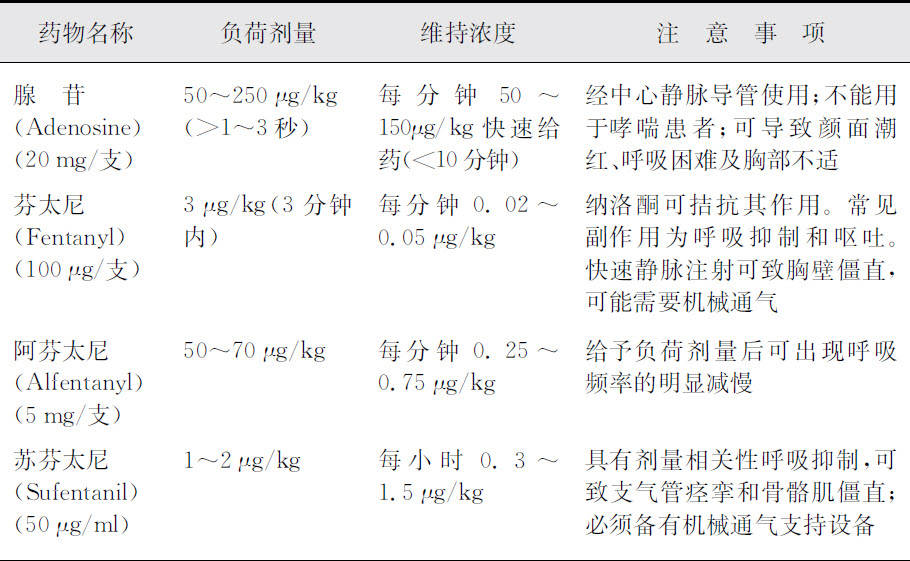
\includegraphics[width=\textwidth,height=\textheight,keepaspectratio]{./images/Image00323.jpg}\\
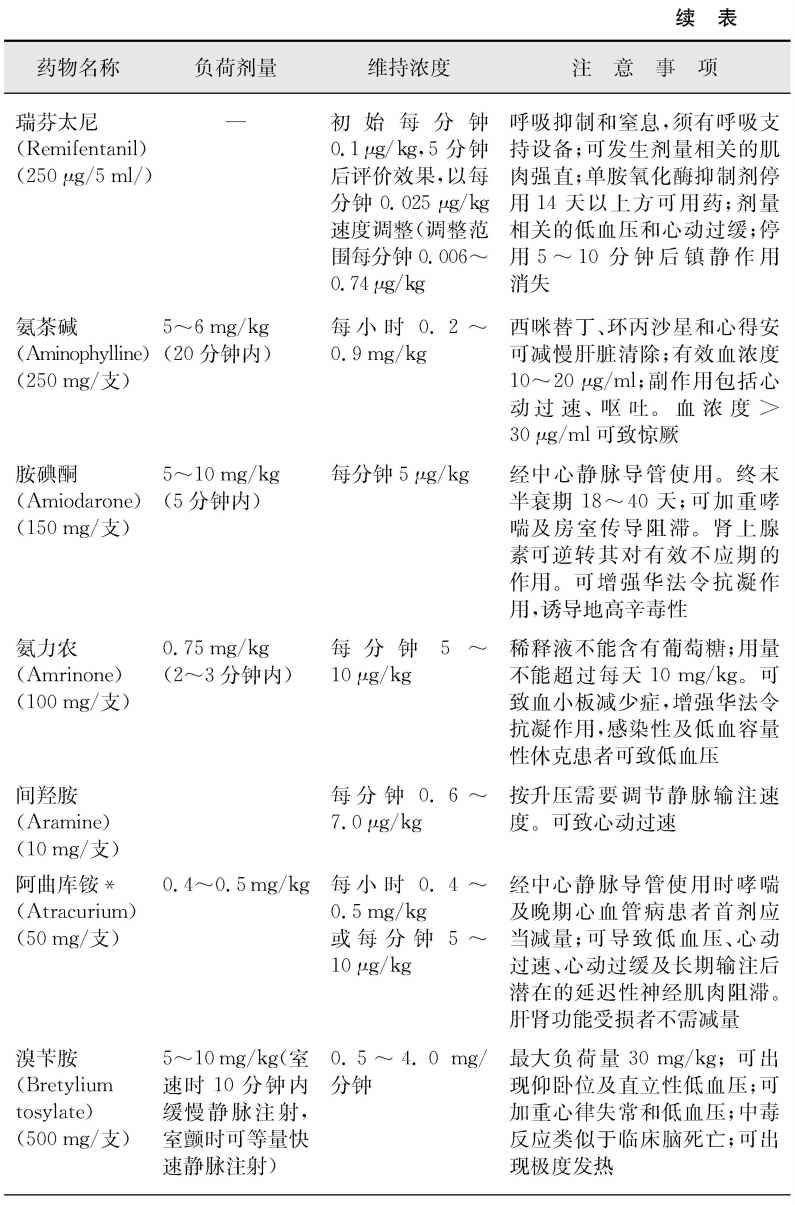
\includegraphics[width=\textwidth,height=\textheight,keepaspectratio]{./images/Image00324.jpg}\\
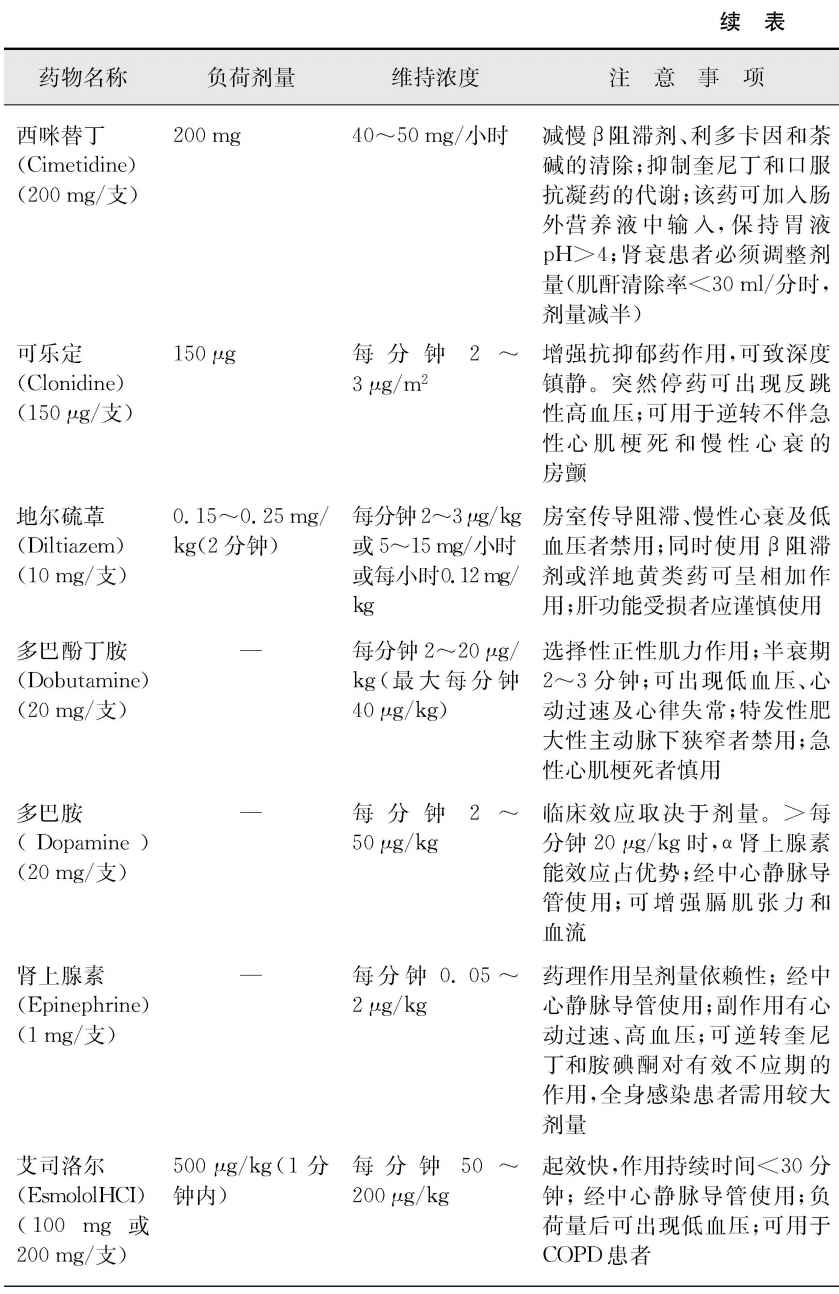
\includegraphics[width=\textwidth,height=\textheight,keepaspectratio]{./images/Image00325.jpg}\\
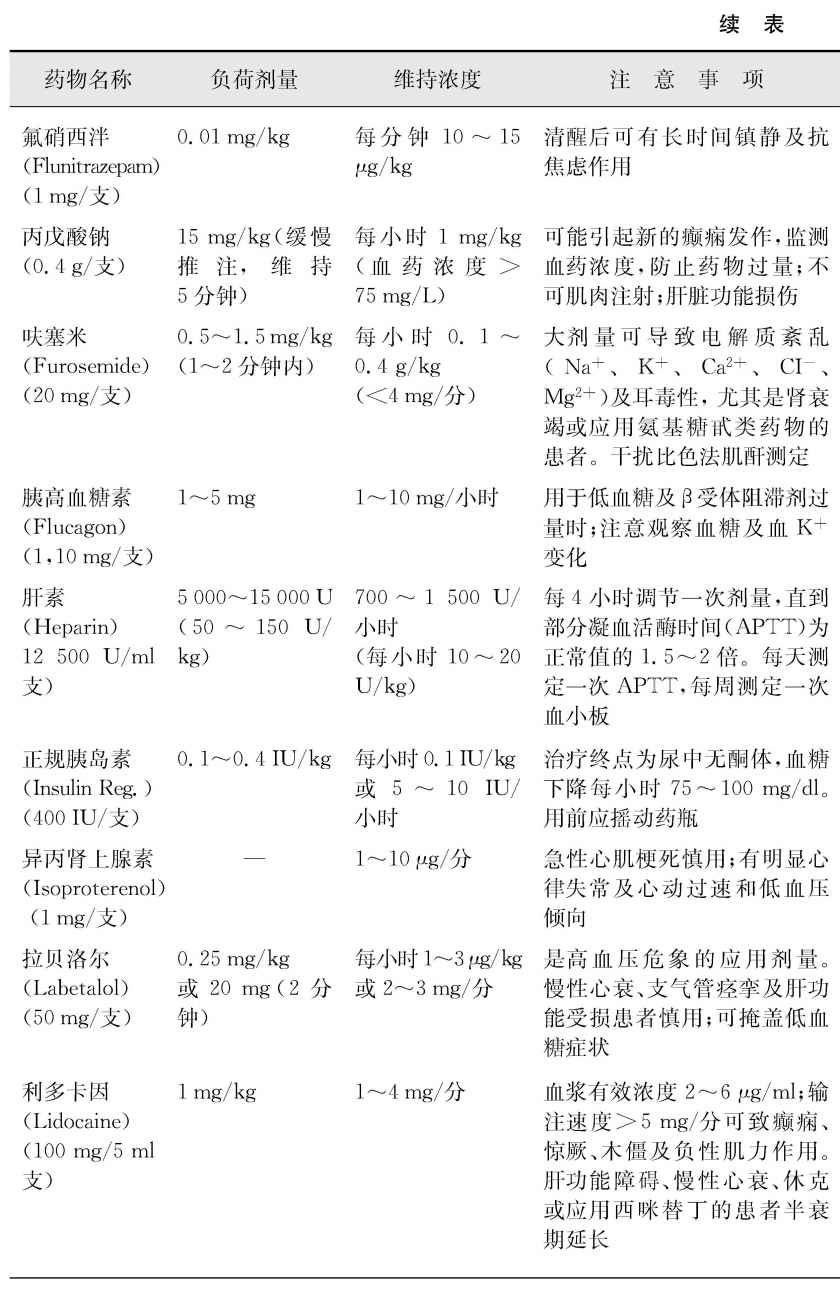
\includegraphics[width=\textwidth,height=\textheight,keepaspectratio]{./images/Image00326.jpg}\\
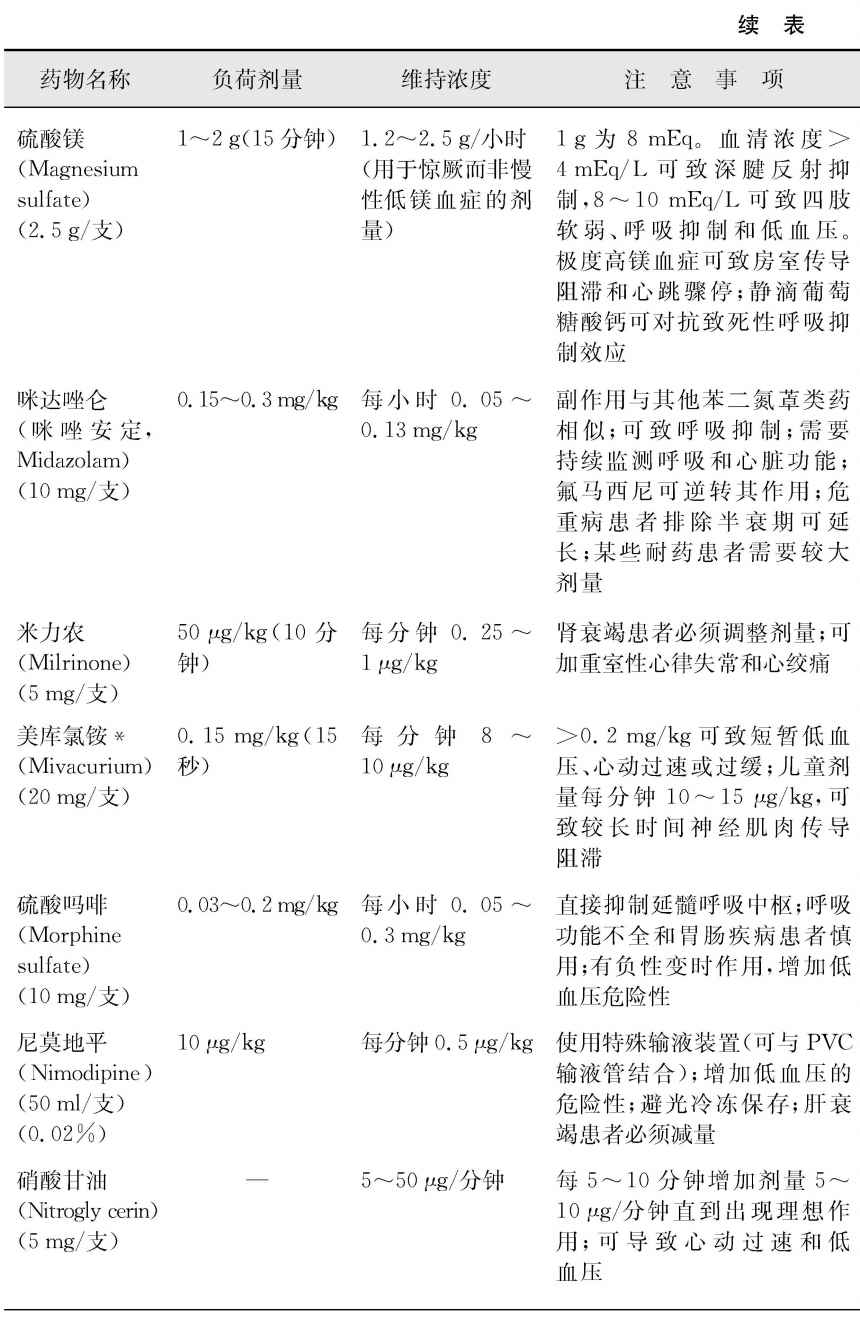
\includegraphics[width=\textwidth,height=\textheight,keepaspectratio]{./images/Image00327.jpg}\\
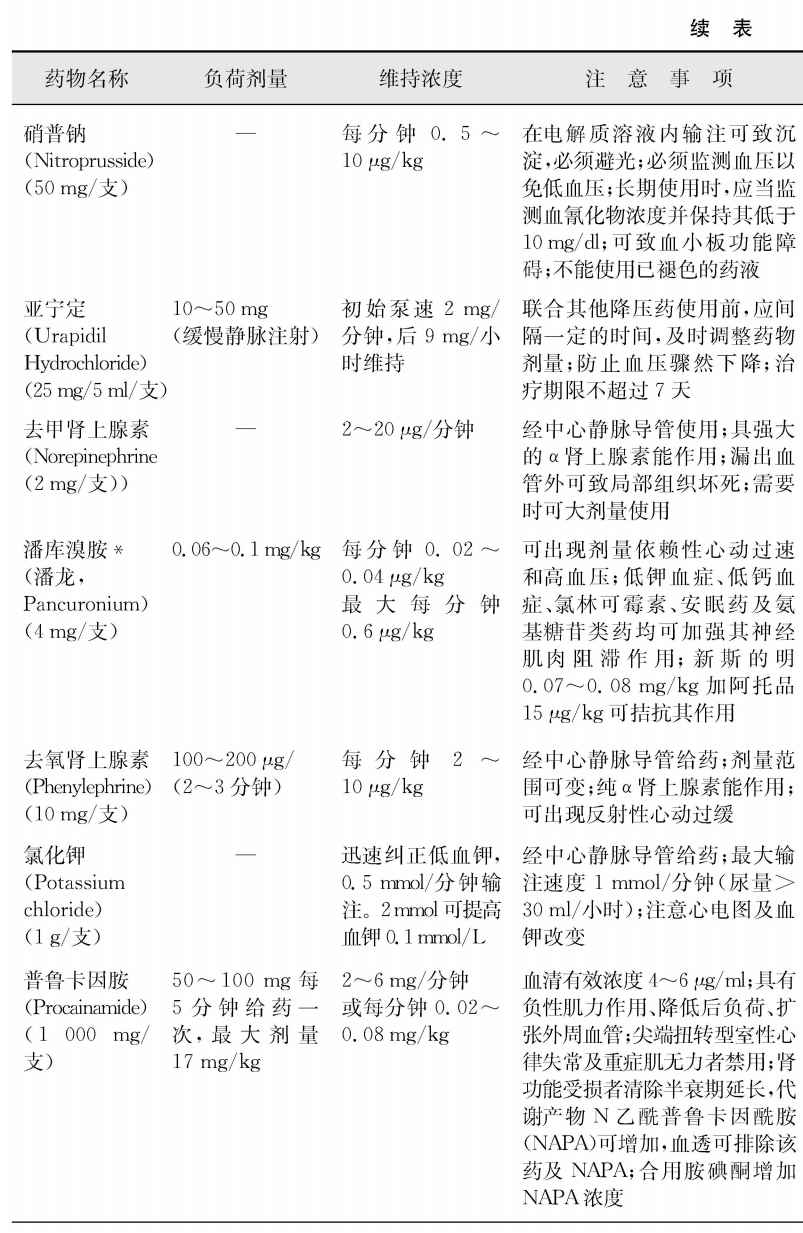
\includegraphics[width=\textwidth,height=\textheight,keepaspectratio]{./images/Image00328.jpg}\\
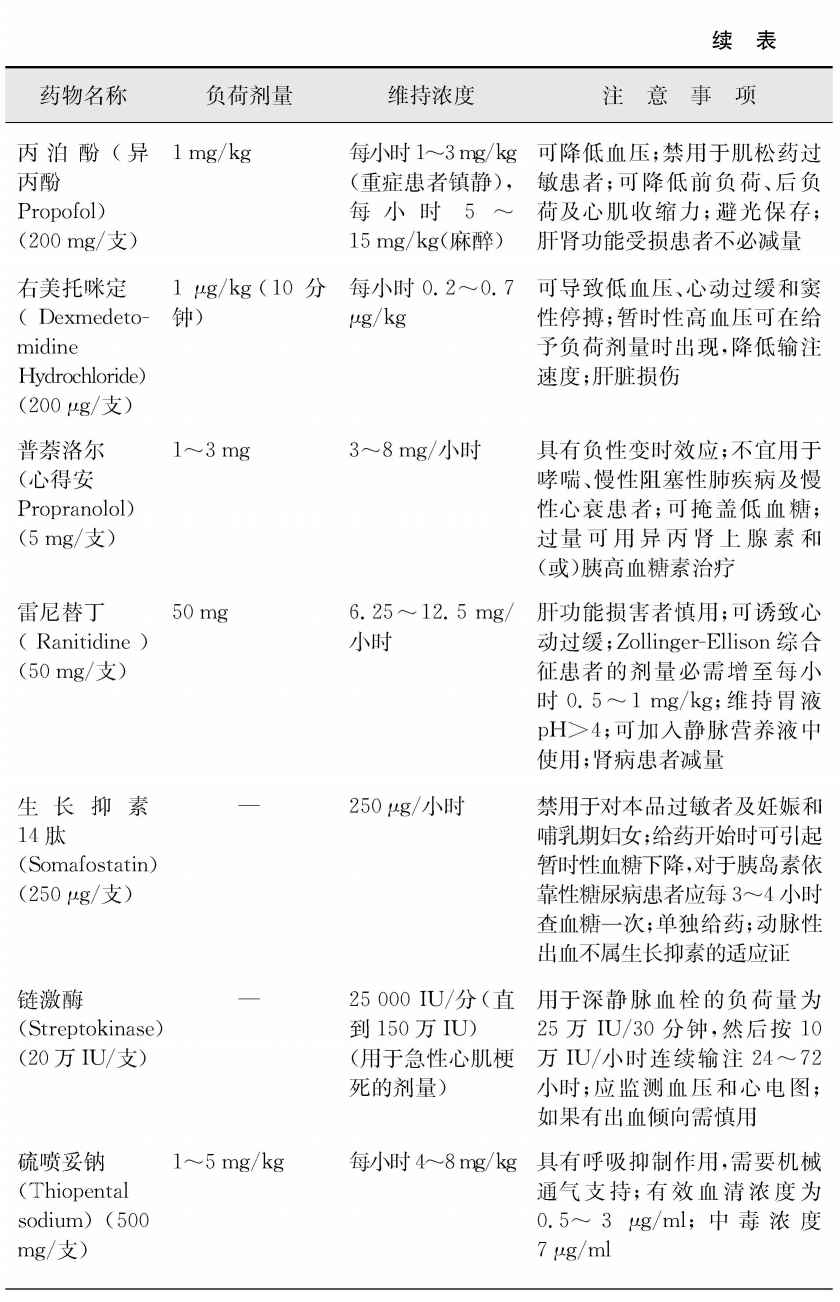
\includegraphics[width=\textwidth,height=\textheight,keepaspectratio]{./images/Image00329.jpg}\\
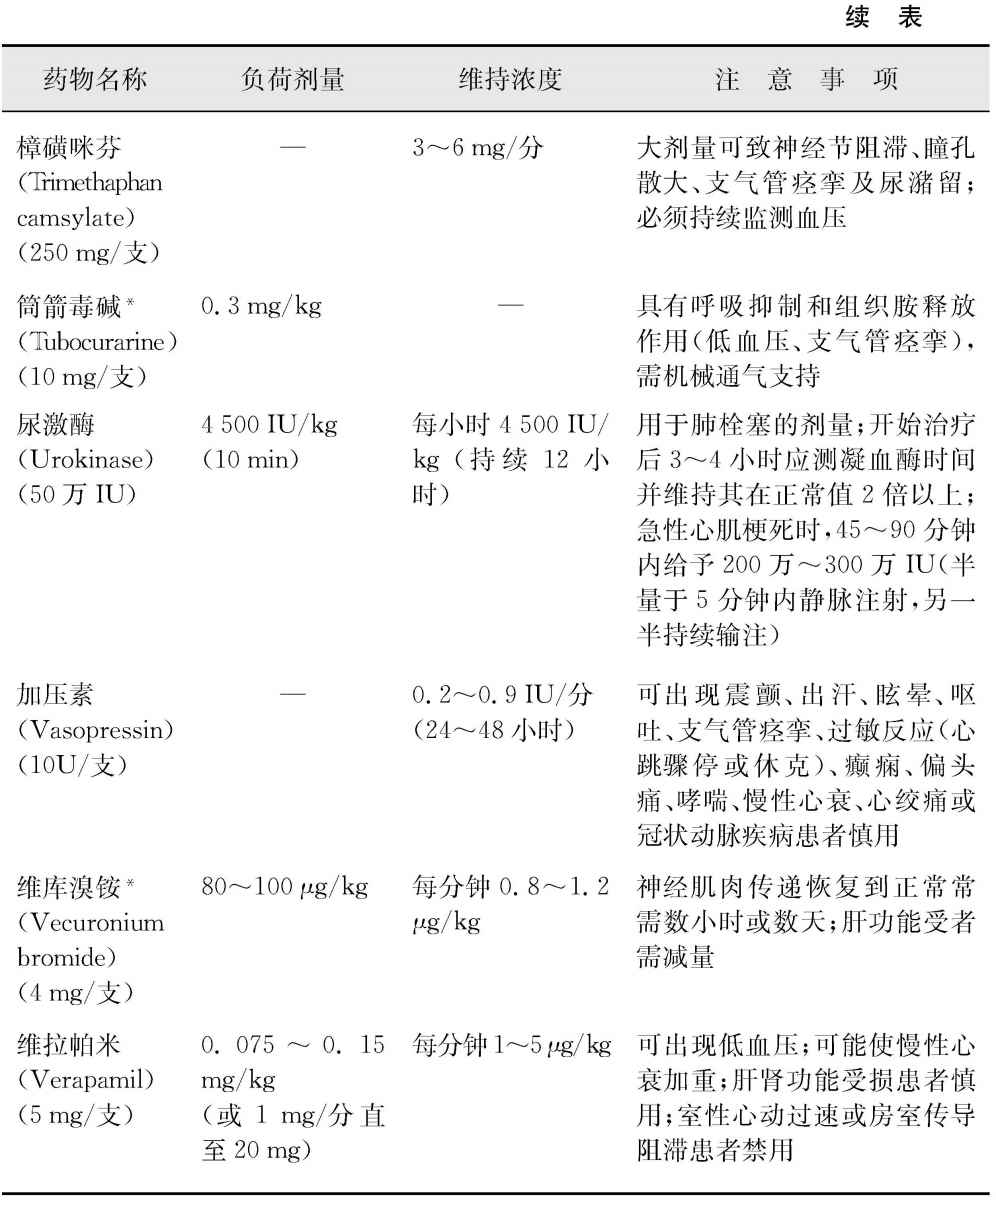
\includegraphics[width=\textwidth,height=\textheight,keepaspectratio]{./images/Image00330.jpg}\\
\end{longtable} 



